\begin{refsection}
\chapter{Testing of Laser Written Emitters and Simulations} % better naming required since this is the second experimental chapter now 29/04/2024 is this good enough for you? DYING OUT HERE OH GOD
\section{Emitter Sharpness}
\label{subsec:emitter_sharpness}
In designing the emitter-type structures, the plausibility of measuring field effect emission was examined via electrostatic finite element modelling (FEM) in Comsol Multiphysics. The most critical factor to consider in these simulations was that of the effective cathode tip. Previous work in Oxford has demonstrated conductive graphite wires going down to 400~\si{\nano\metre} in diameter \cite{sun2014}, however the creation of sharp emitters depends upon the cross-sectional area presented at the very end of such a wire. Simple electrostatic simulations were created to estimate the magnitude of the normal electric field experienced by wires ranging from rectangular in appearance with very sharp corners, to wires with the corners tapered off to such a degree that the radius of curvature aligns with the wire diameter. Following these electrostatic models, implementation of Fowler-Nordheim type field-effect emission with a Murphy-Good approximation was implemented to estimate the emitted current corresponding to the normal electric field on the cathodes \cite{Good1956, Kyritsakis2015, Forbes2019}.

\begin{figure}[H]
    \centering
    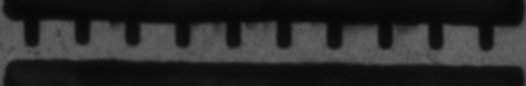
\includegraphics[width=\textwidth]{Chapter7/Figs/ch_channel_esid_tiny.png}
    \caption{The emitter structures of emitter array C-H, as closely examined as possible via oil immersion, 488~\si{\nano\metre} confocal microscopy.}
    \label{fig:ch_tiny_ohgod}
\end{figure}

Figure \ref{fig:ch_tiny_ohgod} shows the laser written emitter structures of interest in emitter structure C-H. While initial modelling was performed without this characterisation, the composition of effective conducting material may differ from the optically distinct profiles formed here. While the diffraction limit is evident on close examination of the emitter structures, further characterisation via experiments utilising conductive atomic force microscopy, or perhaps Kelvin probe force microscopy may provide a much sharper view of the as written emitter tip profiles due to their ability to map the electrical properties that influence field effect emission \cite{Melitz2011, Mikulik2017}.

\begin{figure}[H]
    \centering
    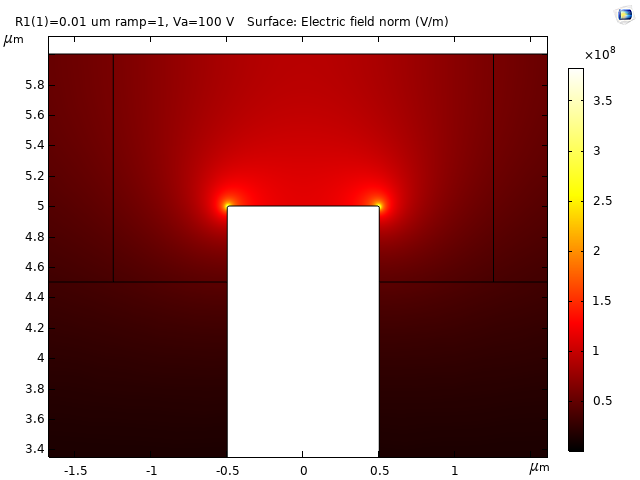
\includegraphics[width=\textwidth]{Chapter7/Figs/Raster/example structure 0.01 normE.png}
    \caption{Electrostatic modelling of a surface graphitic wire with diameter 1~\si{\micro\metre} and corner radii of 0.01~\si{\micro\metre}.}
    \label{fig:comsol_es_wire0.01}
\end{figure}

Figure \ref{fig:comsol_es_wire0.01} illustrates the electrostatic profile of a surface graphitic wire of diameter 1~\si{\micro\metre}, which has very sharp corners which have radii of curvature of 0.01~\si{\micro\metre}. The 2D model is performed with a thickness of 1~\si{\micro\metre}. Note the intensely localised electric field at the corners of the wire, reaching above $3.5\times10^{8}$~\si{\volt\per\metre}, with significantly lower normal electric fields across the rest of the wire. In this model, the cathode is held at 0~\si{\volt}, while the anode is held at 100~\si{\volt}. The cathode-anode spacing is 1~\si{\micro\metre}. The segmented sections visible (black lines) indicate different regions of meshing, with a very dense mesh used for the region immediately surrounding the tip of the emitter to better resolve the sharper features.

\begin{figure}[H]
    \centering
    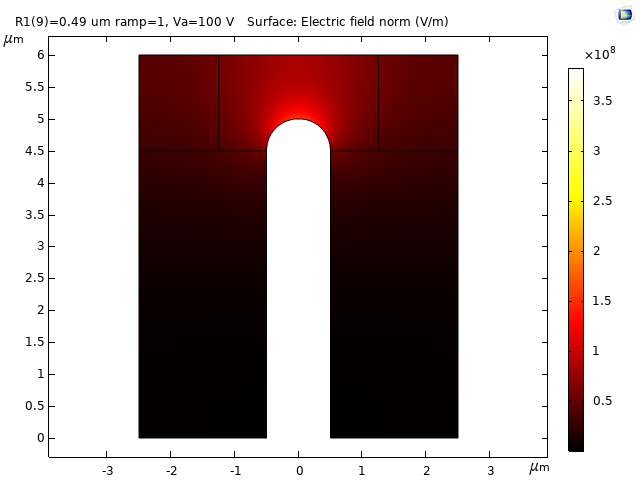
\includegraphics[width=\textwidth]{Chapter7/Figs/Raster/example structure 0.49 normE.png}
    \caption{Electrostatic modelling of a surface graphitic wire with diameter 1~\si{\micro\metre} and corner radii of 0.49~\si{\micro\metre}.}
    \label{fig:comsol_es_wire0.49}
\end{figure}

Figure \ref{fig:comsol_es_wire0.49} demonstrates the electrostatic profile of a surface graphitic wire of diameter 1~\si{\micro\metre}, which has corners of radii 0.49~\si{\micro\metre}. The 2D model is performed with a thickness of 1~\si{\micro\metre}. Note that in contrast to figure \ref{fig:comsol_es_wire0.01}, the wire in this model has corner radii which are very close to the radius of the wire, resulting in a nearly semi-circular end to the wire. The resulting normal electric field is significantly more diffuse than in the low radii example, with a peak at the very end of the wire corresponding to around $1.5\times10^{8}$~\si{\volt\per\metre}. In this model, the cathode is held at 0~\si{\volt}, while the anode is held at 100~\si{\volt}. The cathode-anode spacing is 1~\si{\micro\metre}. The segmented sections that are partially visible (black lines) indicate different regions of meshing, with a very dense mesh used for the region immediately surrounding the tip of the emitter to better resolve the sharper features.

\begin{figure}[H]
    \centering
    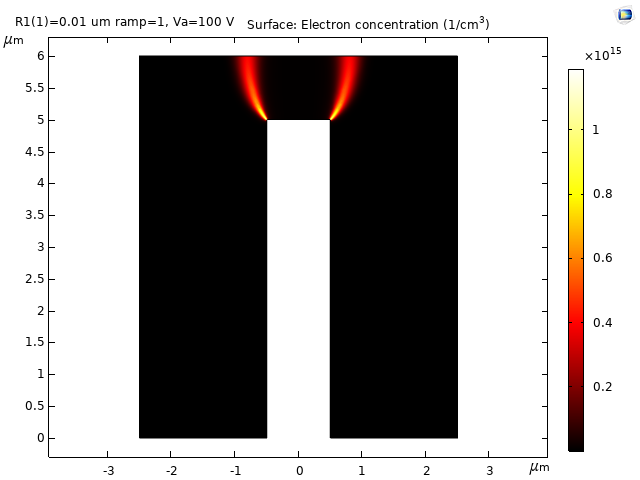
\includegraphics[width=\textwidth]{Chapter7/Figs/Raster/FN radius 0.01 width 1um 100V 0V.png}
    \caption{Fowler-Nordheim modelling of a surface graphitic wire with diameter 1~\si{\micro\metre} and corner radii of 0.01~\si{\micro\metre}.}
    \label{fig:comsol_fn_wire0.01}
\end{figure}

In figure \ref{fig:comsol_fn_wire0.01}, a 2D simulation of a surface graphitic emitter-type structure is shown. Following a Fowler-Nordheim type field-effect emission, the resulting electron concentration can be seen to be heavily emitted from the corners, which have radii of 0.01~\si{\micro\metre}. Notable differences from the previous electrostatic modelling include the implementation of n-type doping corresponding to TLM measurements (exact concentration was what again? maybe refer to section in which I establish modelling and include the TLM models there) and a standard thermionic Schottky barrier at the cathode-diamond interface with the addition of Fowler-Nordheim tunnelling. For more details regarding the computational implementation of Fowler-Nordheim barriers, please see section (bit on meshing, Schottky barriers, some more plots of simple devices, etc. also maybe get better plots of these models, all files still saved no reason why not. normalised colour scale?). The peak electron concentration for this model was just over $1\times10^{15}$~\si{\per\centi\metre\cubed}, which is present at the corners, dropping off rapidly as the peak electric field drops following the electrostatic model of figure \ref{fig:comsol_es_wire0.01}.

\begin{figure}[H]
    \centering
    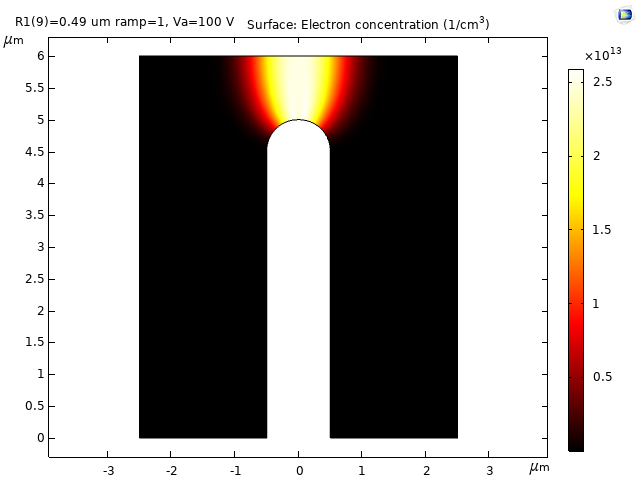
\includegraphics[width=\textwidth]{Chapter7/Figs/Raster/FN radius 0.49 width 1um 100V 0V.png}
    \caption{Fowler-Nordheim modelling of a surface graphitic wire with diameter 1~\si{\micro\metre} and corner radii of 0.49~\si{\micro\metre}.}
    \label{fig:comsol_fn_wire0.49}
\end{figure}

In figure \ref{fig:comsol_fn_wire0.49}, a 2D simulation of a surface graphitic emitter-type structure is shown. Contrasting with figure \ref{fig:comsol_fn_wire0.01}, this model has corners of radii 0.49~\si{\micro\metre}, which are very close to the radius of the wire and hence produce a semi-circular tip. As the Fowler-Norheim emission is highly sensitive to the normal electric field, the peak electron concentration is distributed across the peak of the spherical emitter tip, where a significantly wider region is actively emitting electrons at peak concentration relative to the 0.01~\si{\micro\metre} radii. The peak concentration of electrons in this larger radii case is just over $2.5\times10^{13}$~\si{\per\centi\metre\cubed}, contrasting with the $1\times10^{15}$~\si{\per\centi\metre\cubed} of the sharper case. The order of magnitude difference of 100 with only a scale difference in the peak normal electric field of around 2 demonstrates the drastic geometric enhancement that is possible for field-effect emission.

\section{Laser Written Emitters - Design}
As discussed in section \ref{subsec:field_effect_emission}, laser processing with the aim of producing graphitised wires on the surface or within the bulk of diamond may be used to fabricate devices that rely upon geometric enhancement and hence field effect emission. Simulations indicated that an appreciable level of Fowler-Nordheim type tunnelling is feasible with the small dimensions of laser fabricated wires in diamond \cite{sun2014}. Hence, to test this prediction experimentally, arrays of sharp emitters were designed in a similar fashion to that of LTLM contacts, to provide direct reference data to check for the presence of field effect emission current contributions.
\subsection{Microscopy of Emitters Prior to Testing}
\begin{figure}[H]
    \centering
    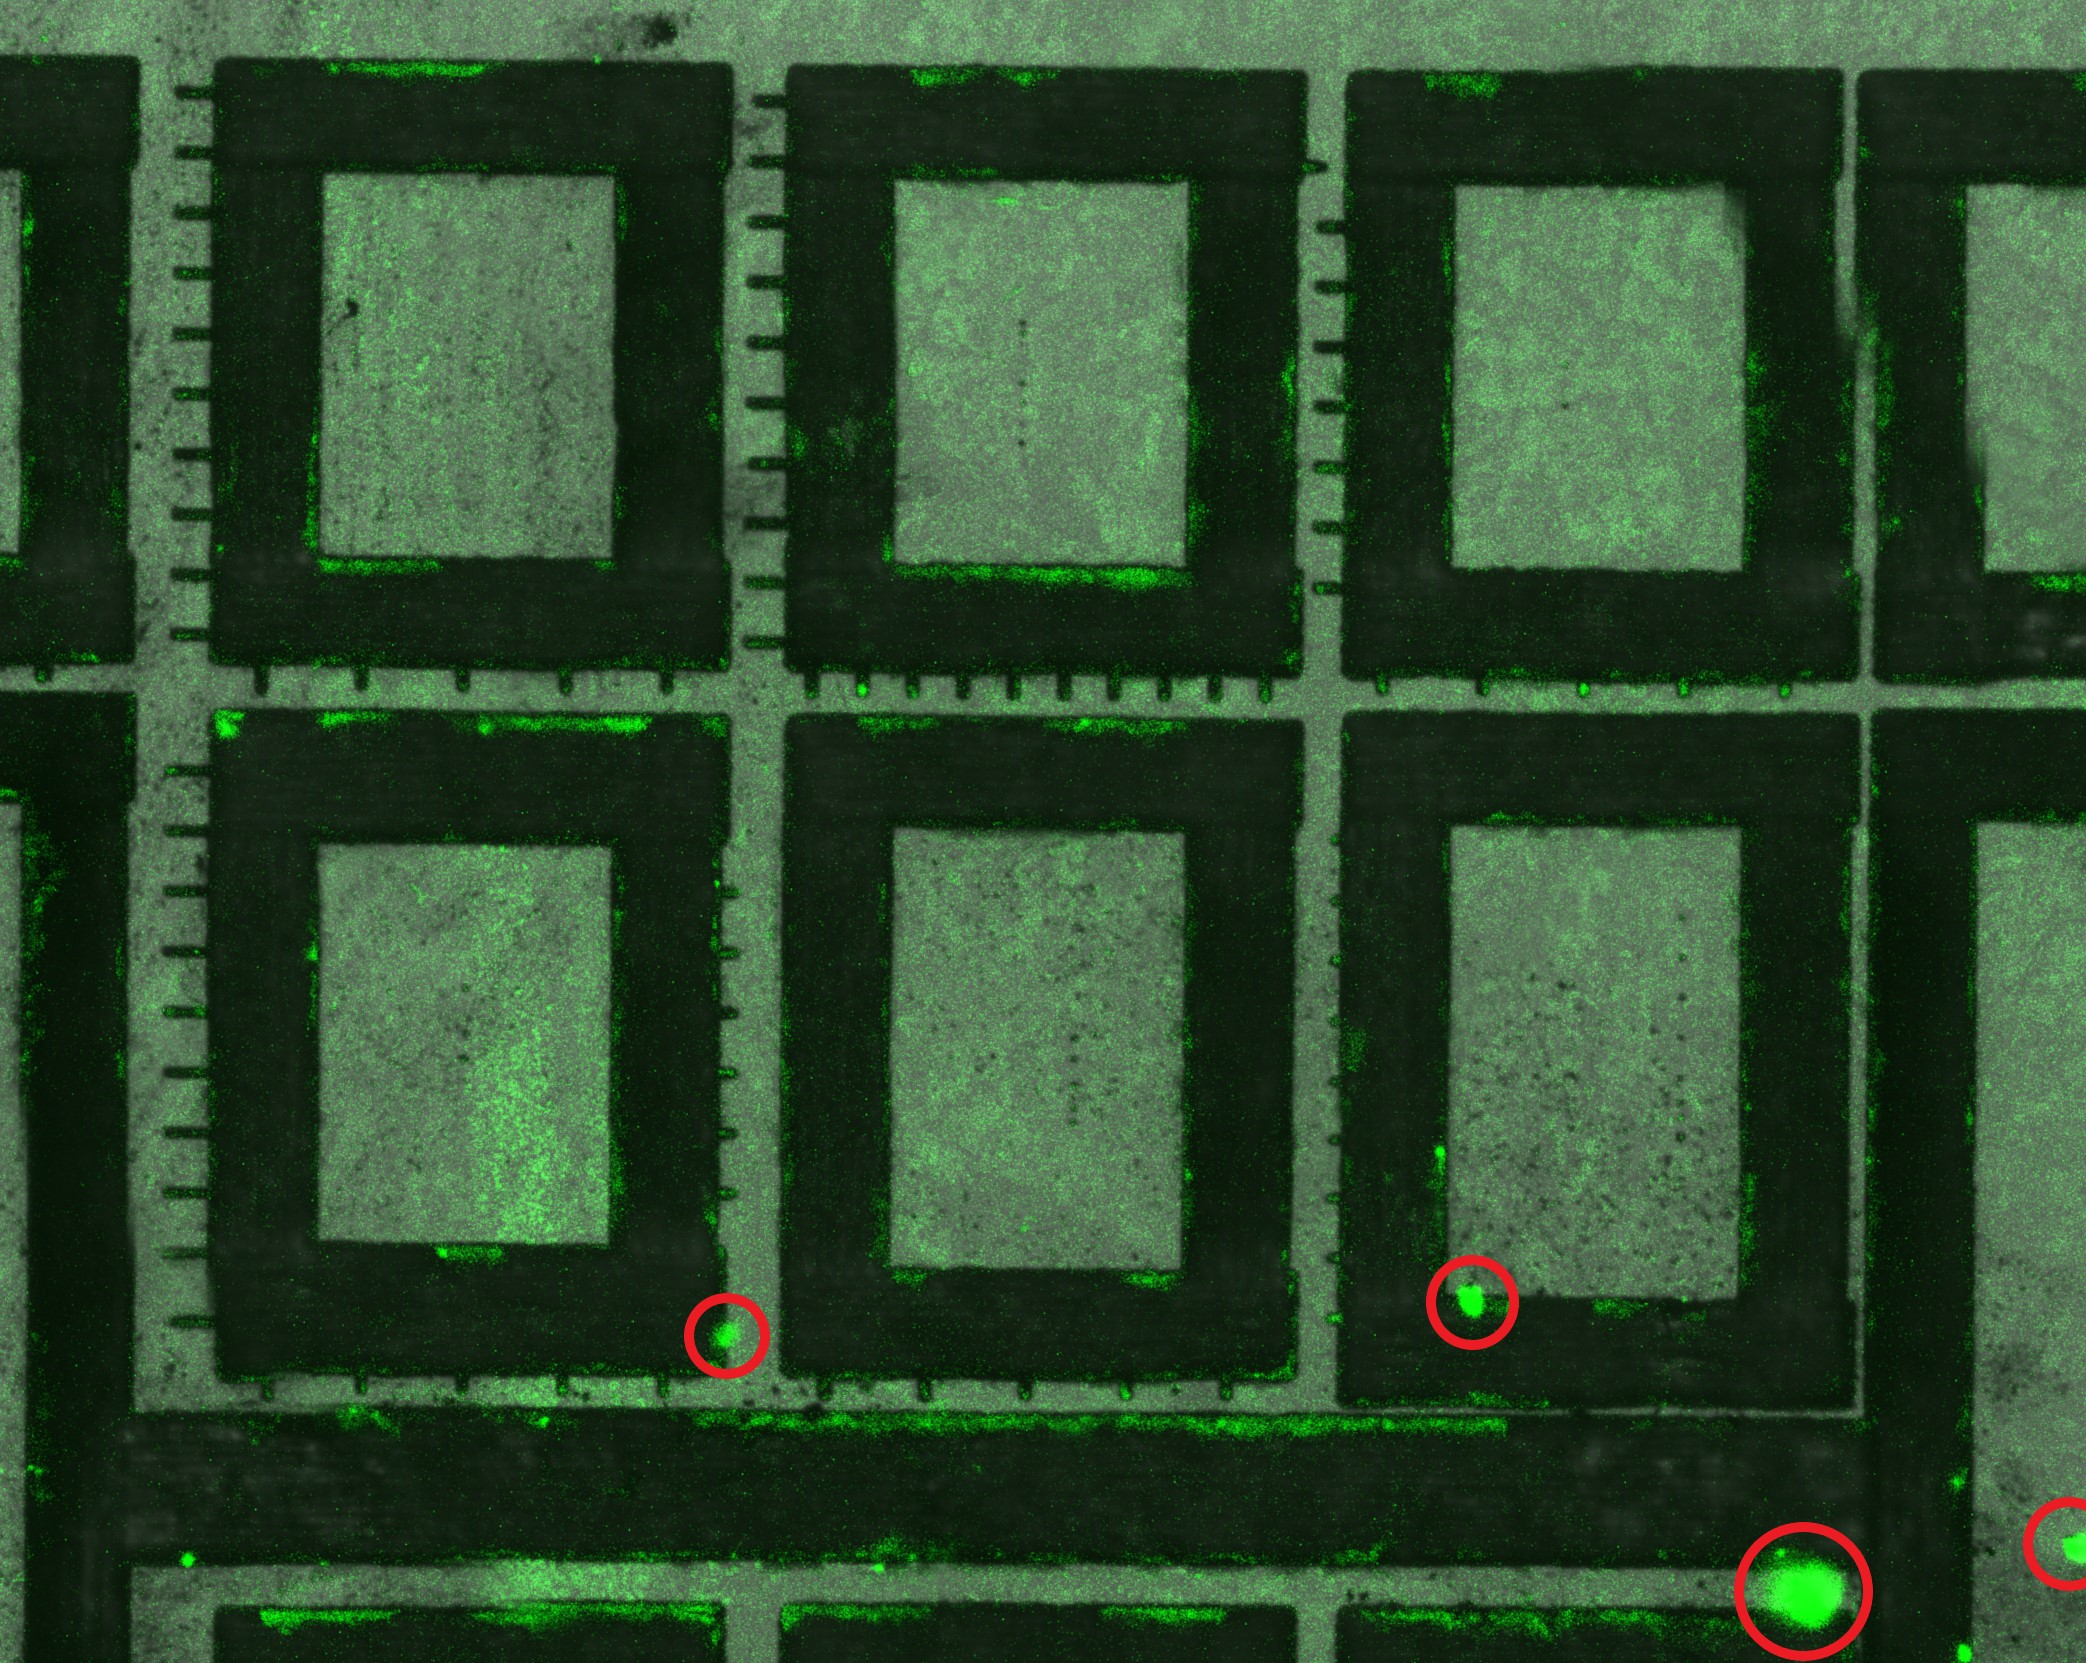
\includegraphics[width=\linewidth]{Chapter7/Figs/Raster/emitter_overview_fl.jpg}
    \caption{An overview of the emitter array structures via confocal microscopy with 488~\si{\nano\metre} laser illumination and 408~\si{\nano\metre} fluorescence.}
    \label{fig:emitter_fl}
\end{figure}

In figure \ref{fig:emitter_fl}, the fluorescence imaging displays the observed fluorescence of these structures. Red circles are used to highlight fluorescence which has previously been speculated to be that of surface contaminants. Please see section \ref{subsec:fluorescence_characterisation} for the full analysis of fluorescence characterisation.

\begin{figure}[H]
    \centering
    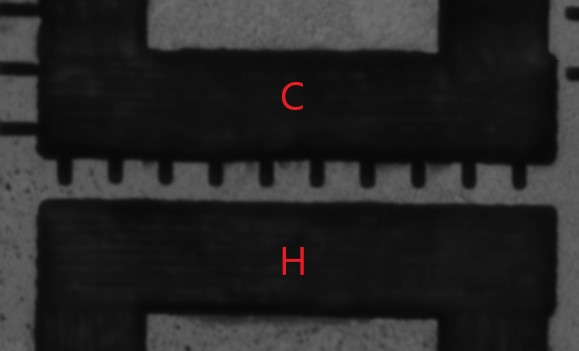
\includegraphics[width=\linewidth]{Chapter7/Figs/Raster/ch_channel_esid.jpg}
    \caption{A cropped view of the CH emission channel, as seen via confocal microscopy with 488~\si{\nano\metre} laser illumination.}
    \label{fig:ch_esid}
\end{figure}

\begin{figure}[H]
    \centering
    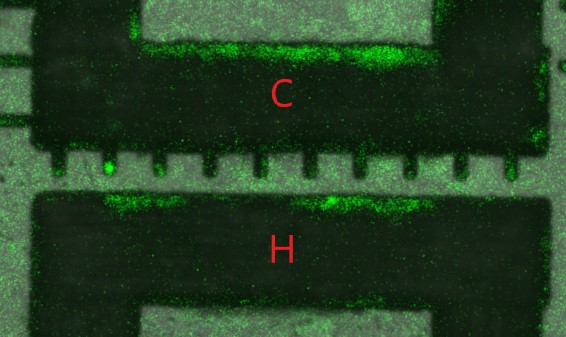
\includegraphics[width=\linewidth]{Chapter7/Figs/Raster/ch_channel_fl.jpg}
    \caption{A cropped view of the CH emission channel, as seen via confocal microscopy with 488~\si{\nano\metre} laser illumination and 408~\si{\nano\metre} fluorescence.}
    \label{fig:ch_fl}
\end{figure}

\begin{figure}[H]
    \centering
    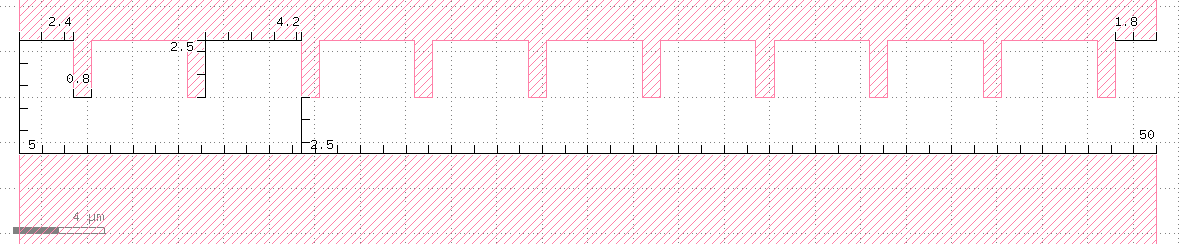
\includegraphics[width=0.8\linewidth]{Chapter7/Figs/Raster/ch_design2.png}
    \caption{The designed channel of emitter channel CH, with measurements of all features.}
    \label{fig:ch_design}
\end{figure}

Figures \ref{fig:ch_esid} and \ref{fig:ch_fl} show the confocal microscopy of the relevant channel, without and with fluorescence respectively. The emitter tip profiles are observed to follow the approximations used in modelling, with the exact radius of curvature for the effective rectangular corners appearing to match that of the expected gaussian beam profile. Due to the difficulty in interpretation of optical microscopy and the exact conductive tips, the more exact geometric profile of these emitters remains difficult to quantify. Figure \ref{fig:ch_design} shows the designed structure of this channel, with emitter wires of thickness 0.8~\si{\micro\metre} chosen in large part due to the enhanced conductivity for slightly wider wire geometries as demonstrated in previous work by Oxford \cite{sun2014}. Thinner wires may have a significantly greater geometric enhancement factor. However, it has been observed that the local resistivity of the written wires is dependent upon the laser fluences used, with natural knock on effects for the cross sectional area of written wires \cite{sun2014}. This is linked to the process of photo and thermal graphitisation, with a summary of the theoretical models in section \ref{subsubsec:thermal_graphitisation}. 

As has been discussed in the previous trial wire measurements from section \ref{subsec:testing_of_surface_graphitic_wires}, some discrepancy even within wide contact wires has been observed that may indicate a difference in sp$^{2}$ conductive carbon allotropes as generated by laser processing on this sample. The difference in observed emitter profiles hence is not unusual, as the exact profile of laser-induced change in carbon allotropes may be sensitive to local crystallinity, which is a factor for the phosphorous-doped surface layer on this sample, as will be examined in section \ref{subsubsec:him_emitters}.

Finally, the fluorescence observed in figure \ref{fig:ch_fl} for emitter array CH has some notable distinguishing features, which raised comparisons to that of AFM topographical mapping.

\begin{figure}[H]
    \centering
    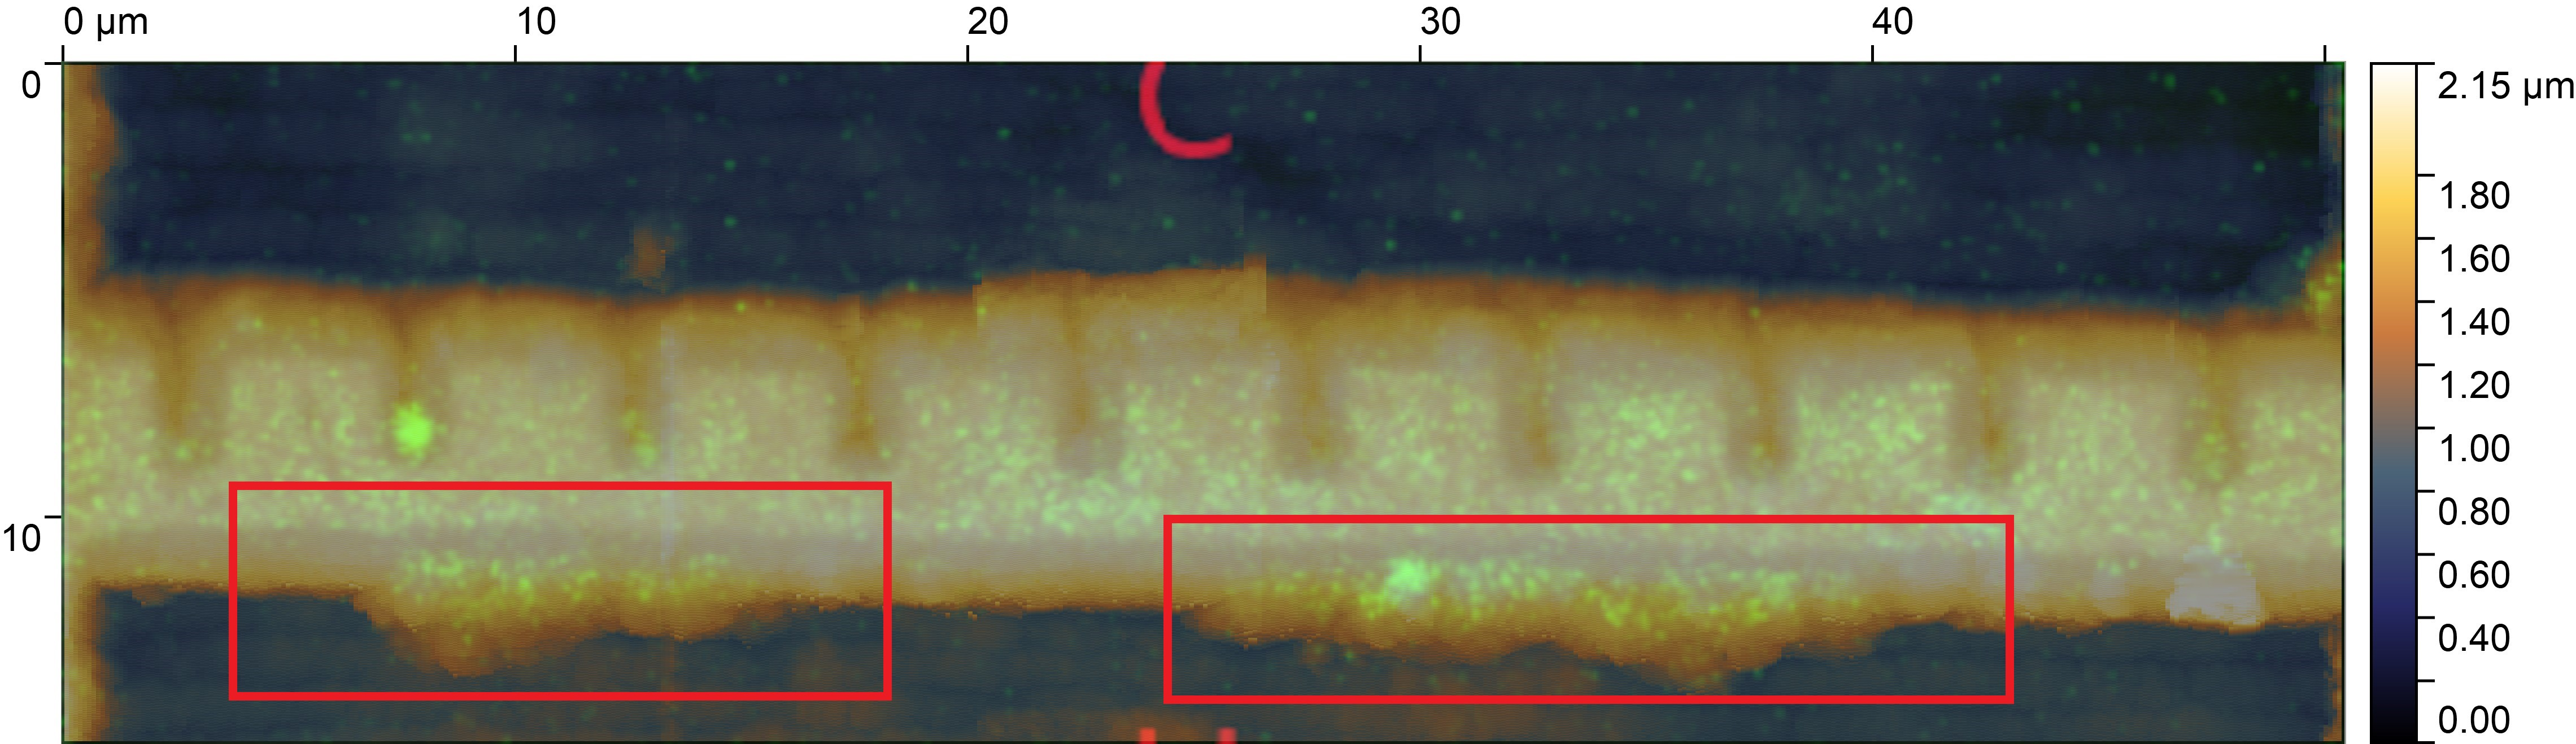
\includegraphics[width=0.8\linewidth]{Chapter7/Figs/Raster/CH_cropped_overlay.jpg}
    \caption{An overlay of the fluorescence observed in channel CH with the AFM topology.}
    \label{fig:ch_overlay}
\end{figure}

Figure \ref{fig:ch_overlay} is a visual overlay of the AFM topology with that of the fluorescence observed. For the AFM topology with no overlay, please see figure \ref{fig:afm_ch_array}. Red rectangles are used to highlight the areas where a high concentration of fluorescence is observed, while also correlating with an edge of contact H which shows a notable change in topology compared to the rest of the laser written contact. If this is material which has not fully undergone thermal graphitisation processes, then it may represent amorphous carbon, from which fluorescence is linked to surface characteristics \cite{Siddique2018, Li2011}.

\subsubsection{Possible Impact of Surface Topology on Emitter Profiles - HIM}
\label{subsubsec:him_emitters}
\begin{figure}[H]
    \centering
    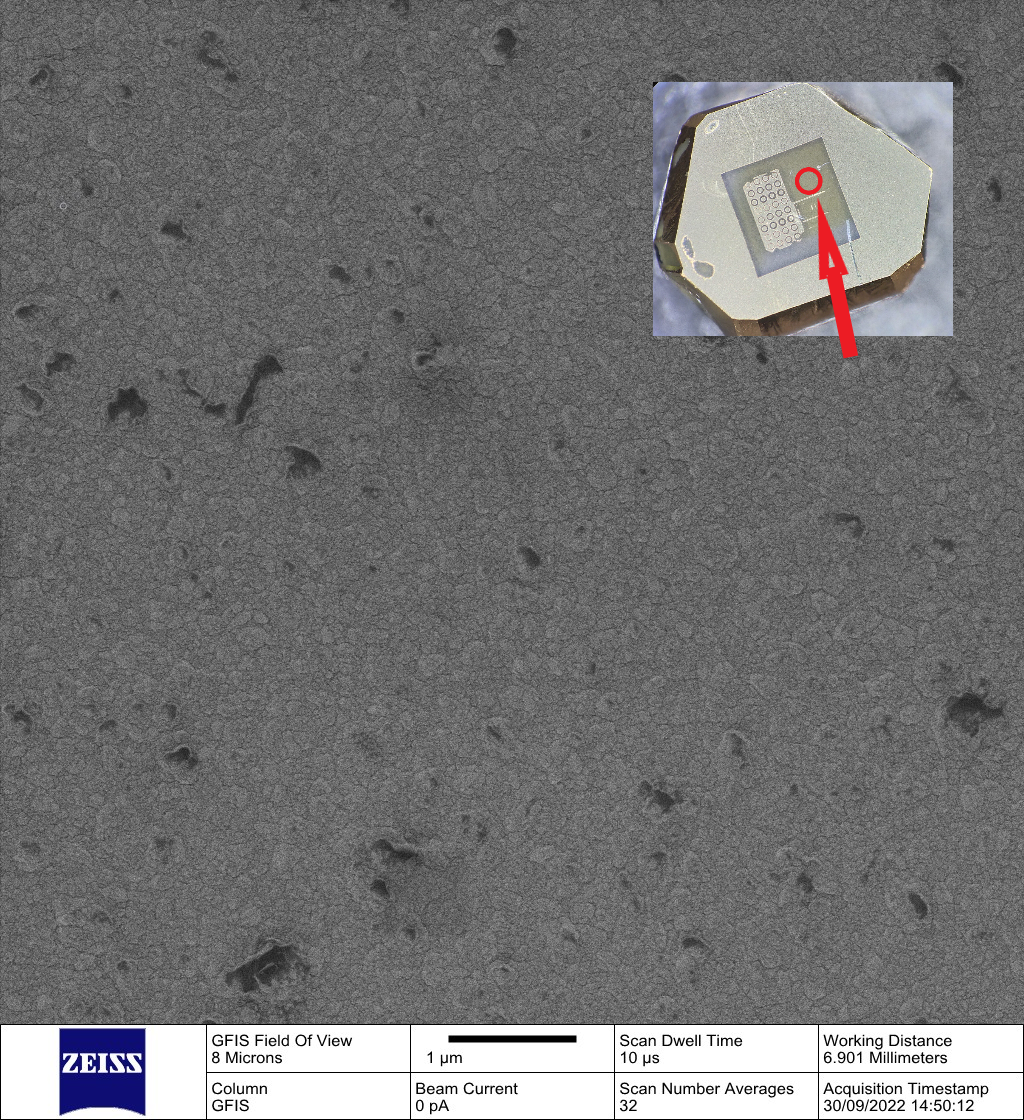
\includegraphics[width=\linewidth]{Chapter7/Figs/Raster/him 002 A.11.jpg}
    \caption{Helium ion microscopy of sample F, as was used for Ti/Au CTLM measurements. Performed in collaboration with NEXUS - Surface characterisation facility at Faculty of SAGE. Inset - picture of sample F with location of HIM marked.}
    \label{fig:him_1}
\end{figure}

To further underscore the crystallinity factor of laser processing and how it may impact the resulting profile of laser induced allotrope changes on the micro-scale, figure \ref{fig:him_1} shows a sample of helium ion microscopy (HIM) that was performed on sample F following CTLM characterisation. This figure is of the highly phosphorous doped diamond surface, which is grown with the same parameters as sample G - the laser processed substrate, with no metal present on this part of the sample. On the scale of $\sim200$~\si{\nano\metre}, multiple "islands" of diamond growth can be seen, corresponding to highly disordered diamond growth with significant concentrations of twinning defects which are typical for \hkl(111) oriented samples \cite{Butler2007, prelas:1997, koizumi1997, koizumi2000, Shechtman1993}. 

One might speculate on the possible role of twinning boundaries and the modification of carbon allotropes via laser processing. Based on the size and shape of these islands, it seems likely that the exact emitter profile is dependent upon the local microstructure within the emitter channel. This would align with theoretical work into the origin of photographitisation processes being primarily defective sites in the diamond lattice \cite{Kononenko2009, kononenko:2015}, but it is unclear on how this may relate to the more recent work on diaphitic allotropes of carbon \cite{salter2024, Nemeth2020, Nemeth20202, Nemeth2021}. Field effect emission from polycrystalline films are a well studied portion of diamond electronic devices \cite{Sugino1998, Watanabe2001, Watanabe2003}, and in particular the internal boundary of phosphorous doped polycrystalline diamond emitters has also been studied previously \cite{Sugino19982}, hence the impact of a relatively polycrystalline surface layer of highly phosphorous doped diamond may be beneficial in the production of high geometric field enhancement, despite the difficulty in producing designs that rely upon planar geometries for exact device properties.

\begin{figure}[H]
    \centering
    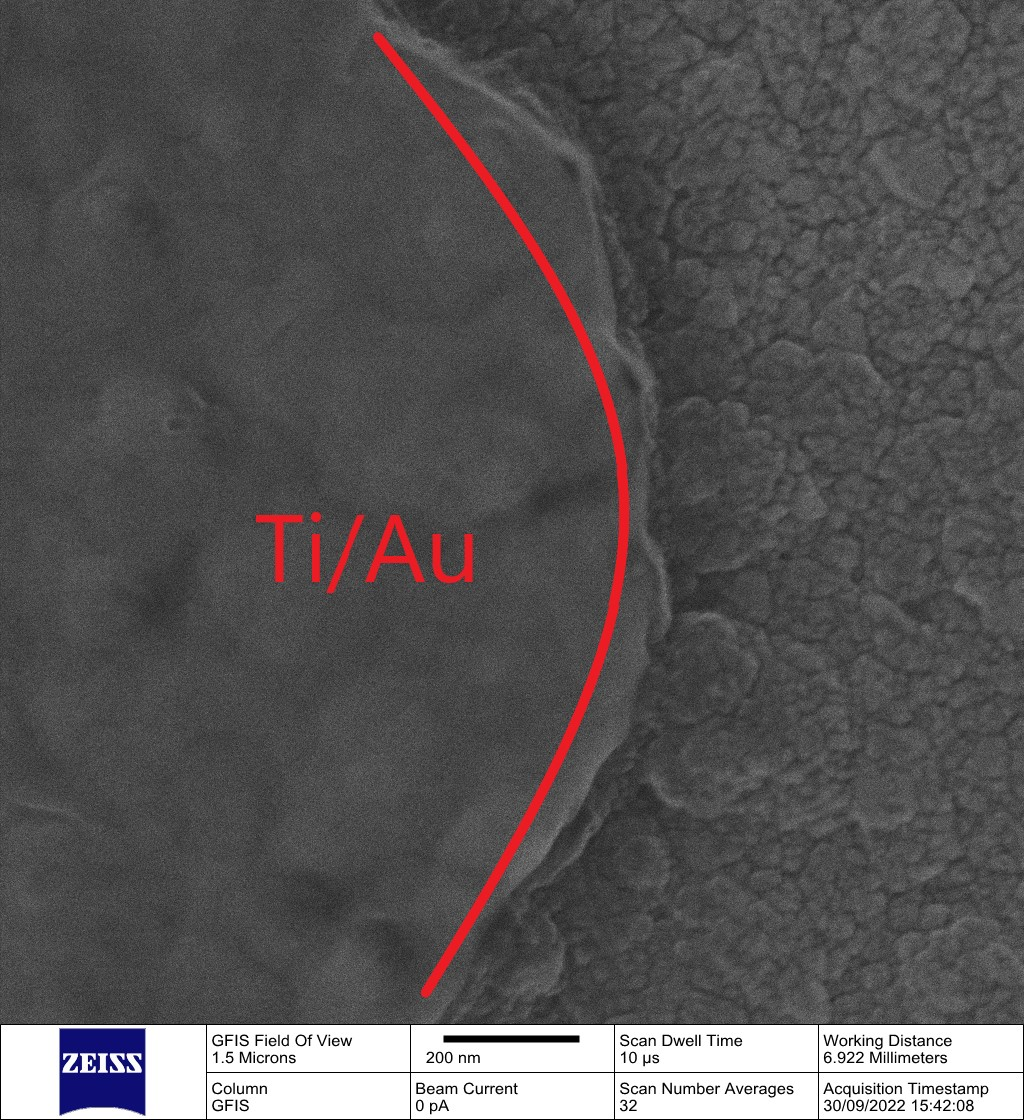
\includegraphics[width=\linewidth]{Chapter7/Figs/Raster/him 007 A.6.jpg}
    \caption{Helium ion microscopy of sample F, as was used for Ti/Au CTLM measurements. Performed in collaboration with NEXUS - Surface characterisation facility at Faculty of SAGE.}
    \label{fig:him_2}
\end{figure}

Figure \ref{fig:him_2} provides another HIM image of sample F, for a scan width of 1.5~\si{\micro\metre} in comparison to the previous width of 8~\si{\micro\metre}. Note the marked region on the left is a Ti/AU contact, while the right side is the uncoated phosphorous doped diamond surface, which displays a complex surface topology on the scale of tens of nanometres to hundreds of nanometres.

\subsection{Possible Impact of Surface Topology on Emitter Profiles - D-AFM and NC-AFM}
One extra set of topology characterisation data were taken via dynamic-AFM or tapping mode AFM on an untreated region of sample G, to provide some evidence that the heavily phosphorous doped surface layer grown on the two samples is similar in crystallinity. Unfortunately, the cantilevers available were the NC-AFM tips used for the earlier AFM topologies in section \ref{subsec:afm_characterisation}. While the depth resolution for previous scans was suitable to detect the surface ablation for emitter wires of width 0.8~\si{\micro\metre} and other such features, the diamond surface required an order of magnitude improvement. Hence, measurements were conducted with a wide sweep of the available adjustable parameters for the XE-150 AFM system, in an attempt to achieve the required resolution with cantilevers that are not suitable for contact-AFM mode characterisation.

\begin{figure}[H]
    \centering
    \begin{subfigure}[b]{0.49\textwidth}
        \centering
        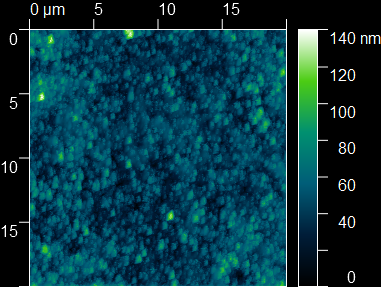
\includegraphics[width=\textwidth]{Chapter7/Figs/Raster/DAFM/forward DFM 55 drive 2 z 256 04 Hz.png}
        \caption{D-AFM scan.}
        \label{fig:dafm}
    \end{subfigure}
    \hfill
    \begin{subfigure}[b]{0.49\textwidth}
        \centering
        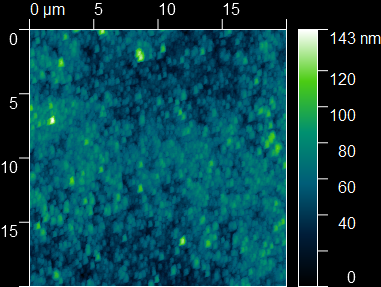
\includegraphics[width=\textwidth]{Chapter7/Figs/Raster/DAFM/forward NC-AFM 100 drive 1 z 256 05 Hz.png}
        \caption{Finely calibrated NC-AFM scan.}
        \label{fig:ncafm}
    \end{subfigure}
    \caption{Comparison of D-AFM and NC-AFM scans of the phosphorous doped diamond surface, in a region that was not subject to laser processing.}
    \label{fig:dafmncafm}
\end{figure}

Figures \ref{fig:dafm} and \ref{fig:ncafm} represent topological testing via D-AFM and NC-AFM respectively. Note that the images are slightly offset due to difficulties with scanning precisely the same region on the diamond sample with no visible surface features. While the HIM images demonstrate a much greater visual clarity on the nano-scale, D-AFM and NC-AFM conducted on a part of the phosphorous doped diamond surface for the laser graphitised sample confirm that there are indeed comparable features with heights of up to around 140~\si{\nano\metre}. While the resolution of these images is lower in comparison to HIM, with an effective pixel area of 78~\si{\nano\metre\squared\per\pixel}, the randomly seeded nature of the as-grown diamond surface seems clear, with some quantification of the difference in height due to these different islands of diamond growth. Of the two contact methodologies employed, the tapping D-AFM mode would be expected to provide a marginally more precise topological map than the NC-AFM mode, however in figure \ref{fig:dafmncafm} it is hard to distinguish the two methodologies. This may be due to the calibration steps taken to reduce noise to an absolute minimum in the NC-AFM mode. Specifically, an absolute minimum level of z-drive was used, with a scan rate of 0.4~\si{\hertz} for both D-AFM and NC-AFM over a resolution of $256x\times56$ pixels corresponding to 78~\si{\nano\metre\squared\per\pixel}. Additionally, several rounds of calibration were performed to reduce noise due to slight mirror misalignments or other such physical parameters. The only distinguishing detail in favour of D-AFM may be the observation of lower average troughs, which should reflect directly on the AFM tip relying on the tipping point of attractive and repulsive Van der Waals forces to identify the correct local heights.

To conclude, surface features visible via HIM and AFM characterisation on the phosphorous doped diamond surface introduce additional complexity into the formation of laser written graphitic structures. The typical diameter of such surface features is of the order of 20 to 200~\si{\nano\metre}, with observed heights of up to 140~\si{\nano\metre}. The emitter tip profiles are contingent upon a thin, sharp ending of the laser written wire. Hence, it is possible that within an emitter array of identical optical profiles, substantial grain boundaries of random orientation and sharpness may either degrade or improve the devices. While this is difficult to account for on a larger scale, this could be a crucial factor.

\section{Emitter Electrical Characteristics}

\begin{figure}[H]
    \centering
    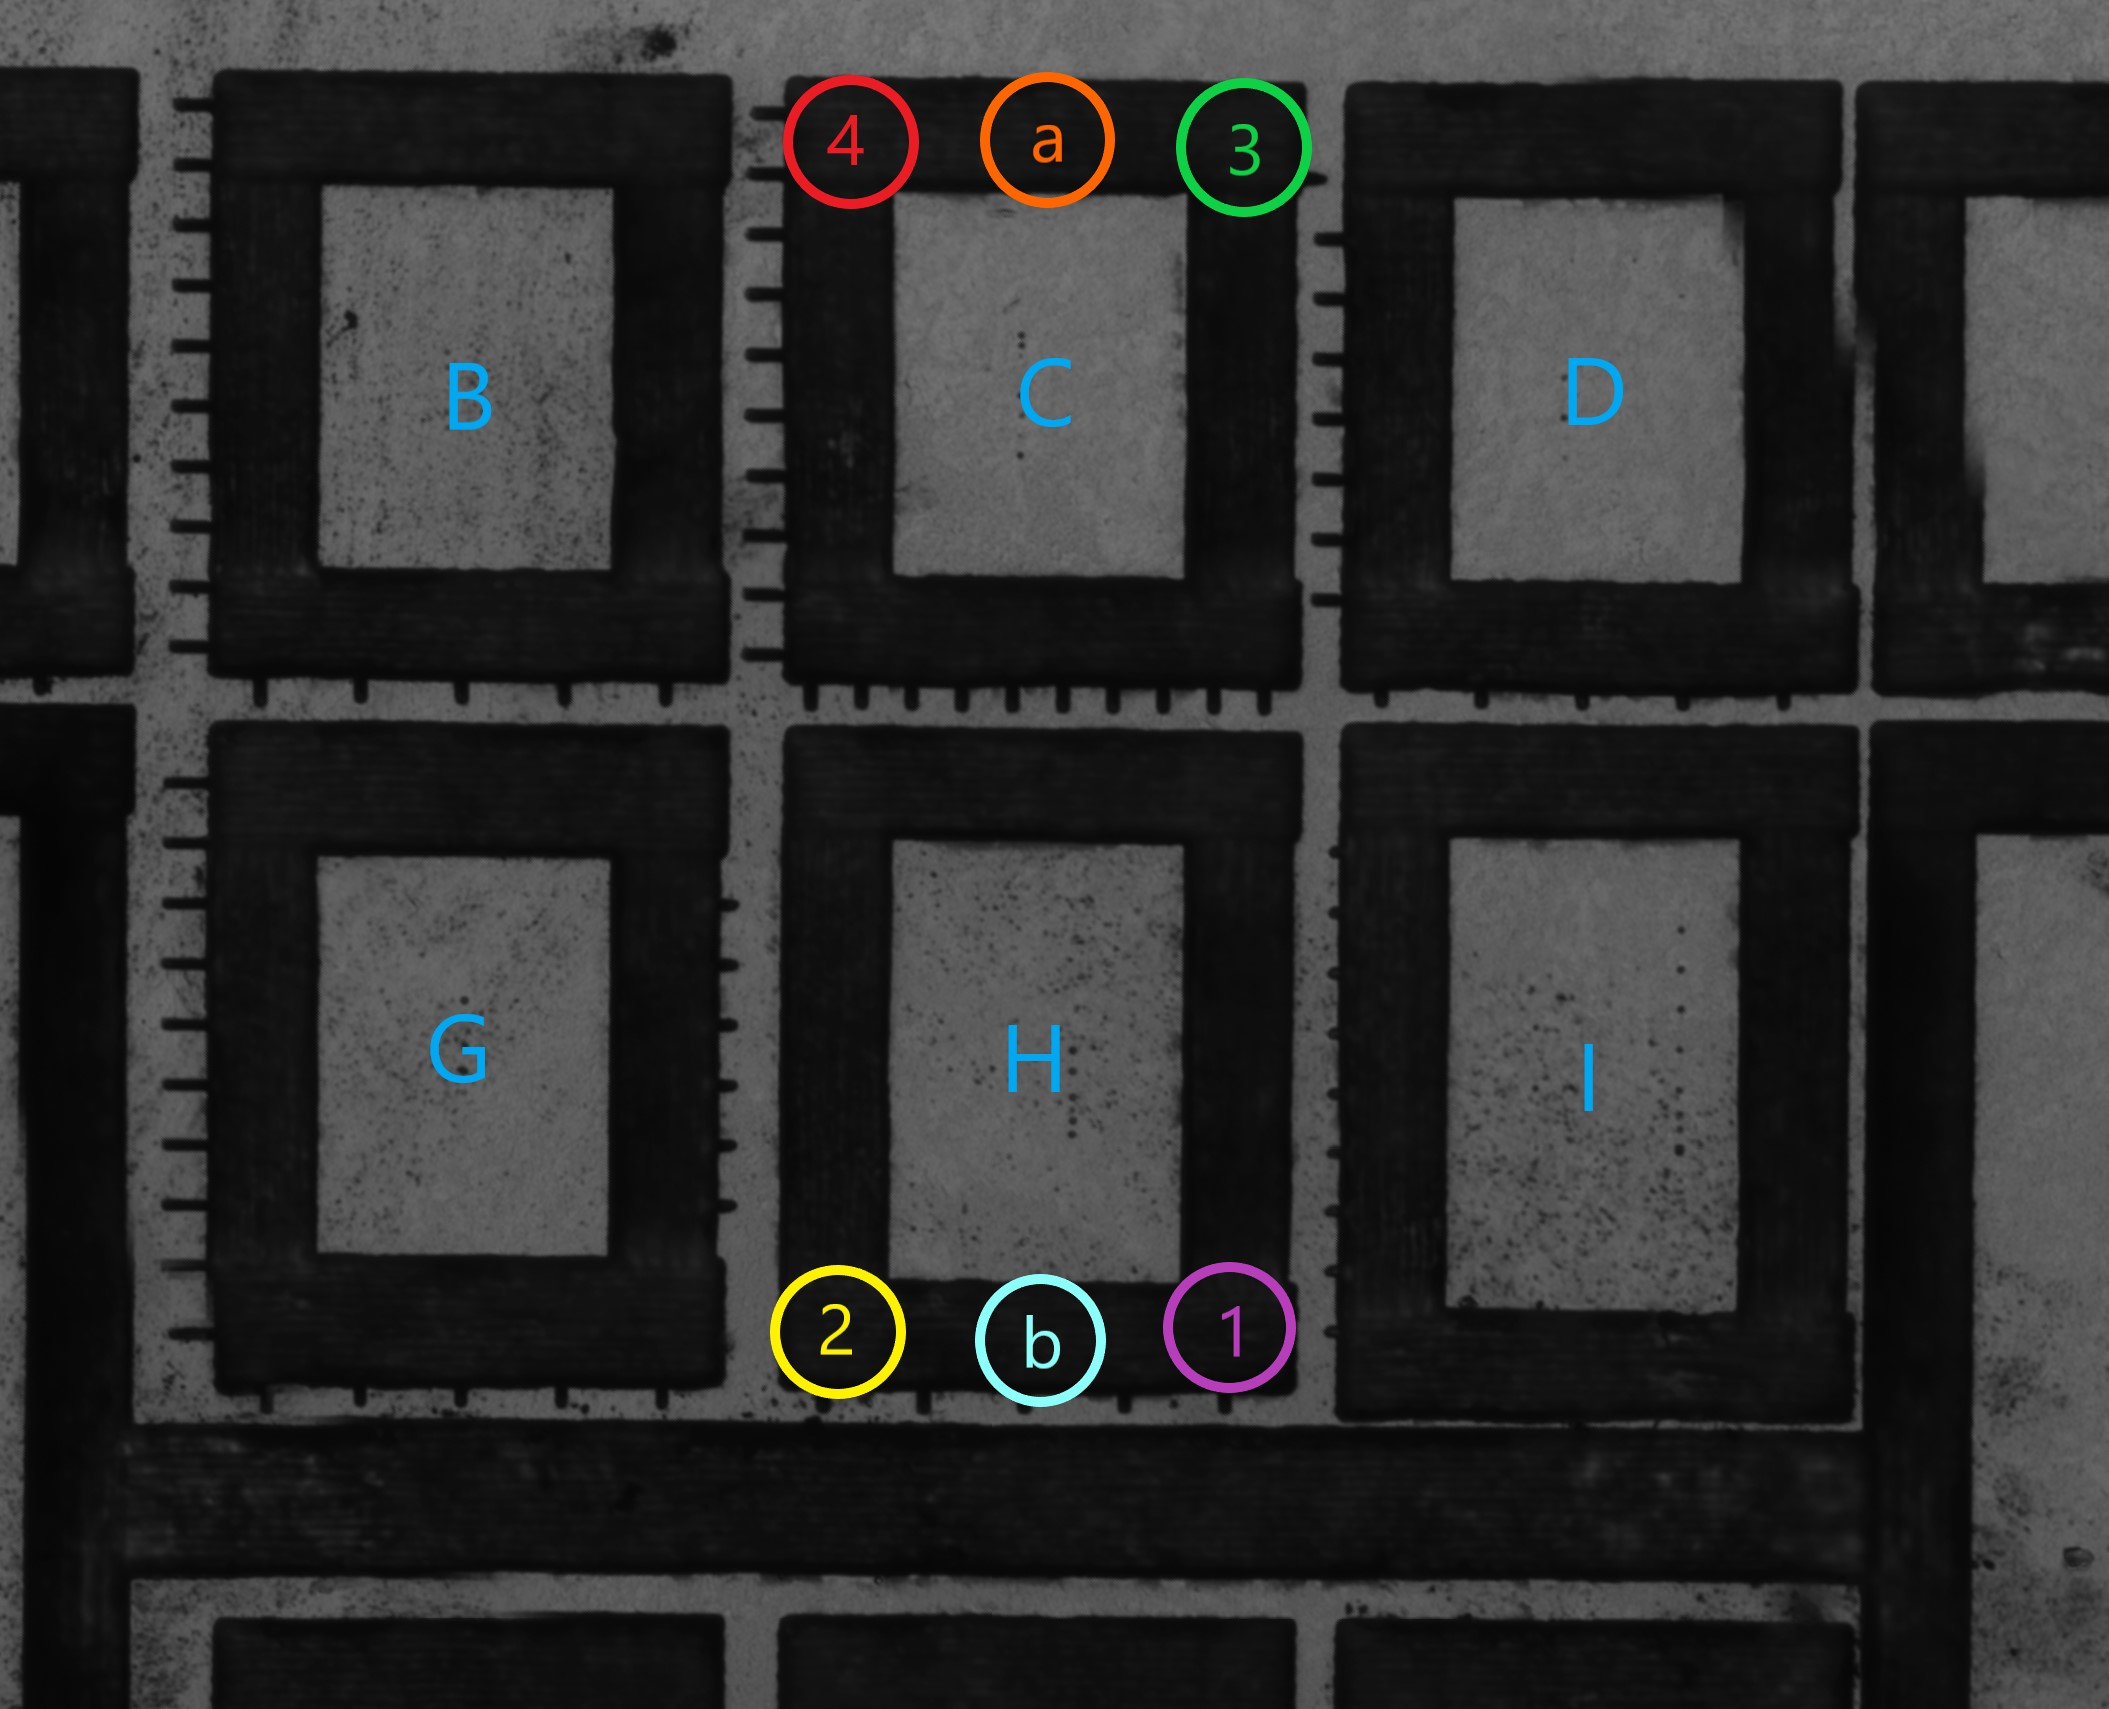
\includegraphics[width=\linewidth]{Chapter7/Figs/Raster/emitter_probes_esid.jpg}
    \caption{An overview of the emitter array structures via confocal microscopy with 488~\si{\nano\metre} laser illumination, and the locations of specific probes during IV characterisation of channel CH.}
    \label{fig:emitter_esid_anno}
\end{figure}

Figure \ref{fig:emitter_esid_anno} provides a view of the relevant emitter contact structures, and their neighbouring contacts as seen with confocal microscopy. Annotations indicate probe positions 1-4 used for the wire verification data, and positions a-b for the high voltage emitter testing.

In the following sections, the verification trials undertaken to ensure good electrical contact to the laser processed wires are summarised. In essence, the core trials involved an IV sweep of a portion of each contact, followed by low voltage sweeps across the emitter channel to verify reasonable magnitudes. 

\subsubsection{Low-Voltage Wire Testing: 4-3}

\begin{figure}[H]
    \centering
    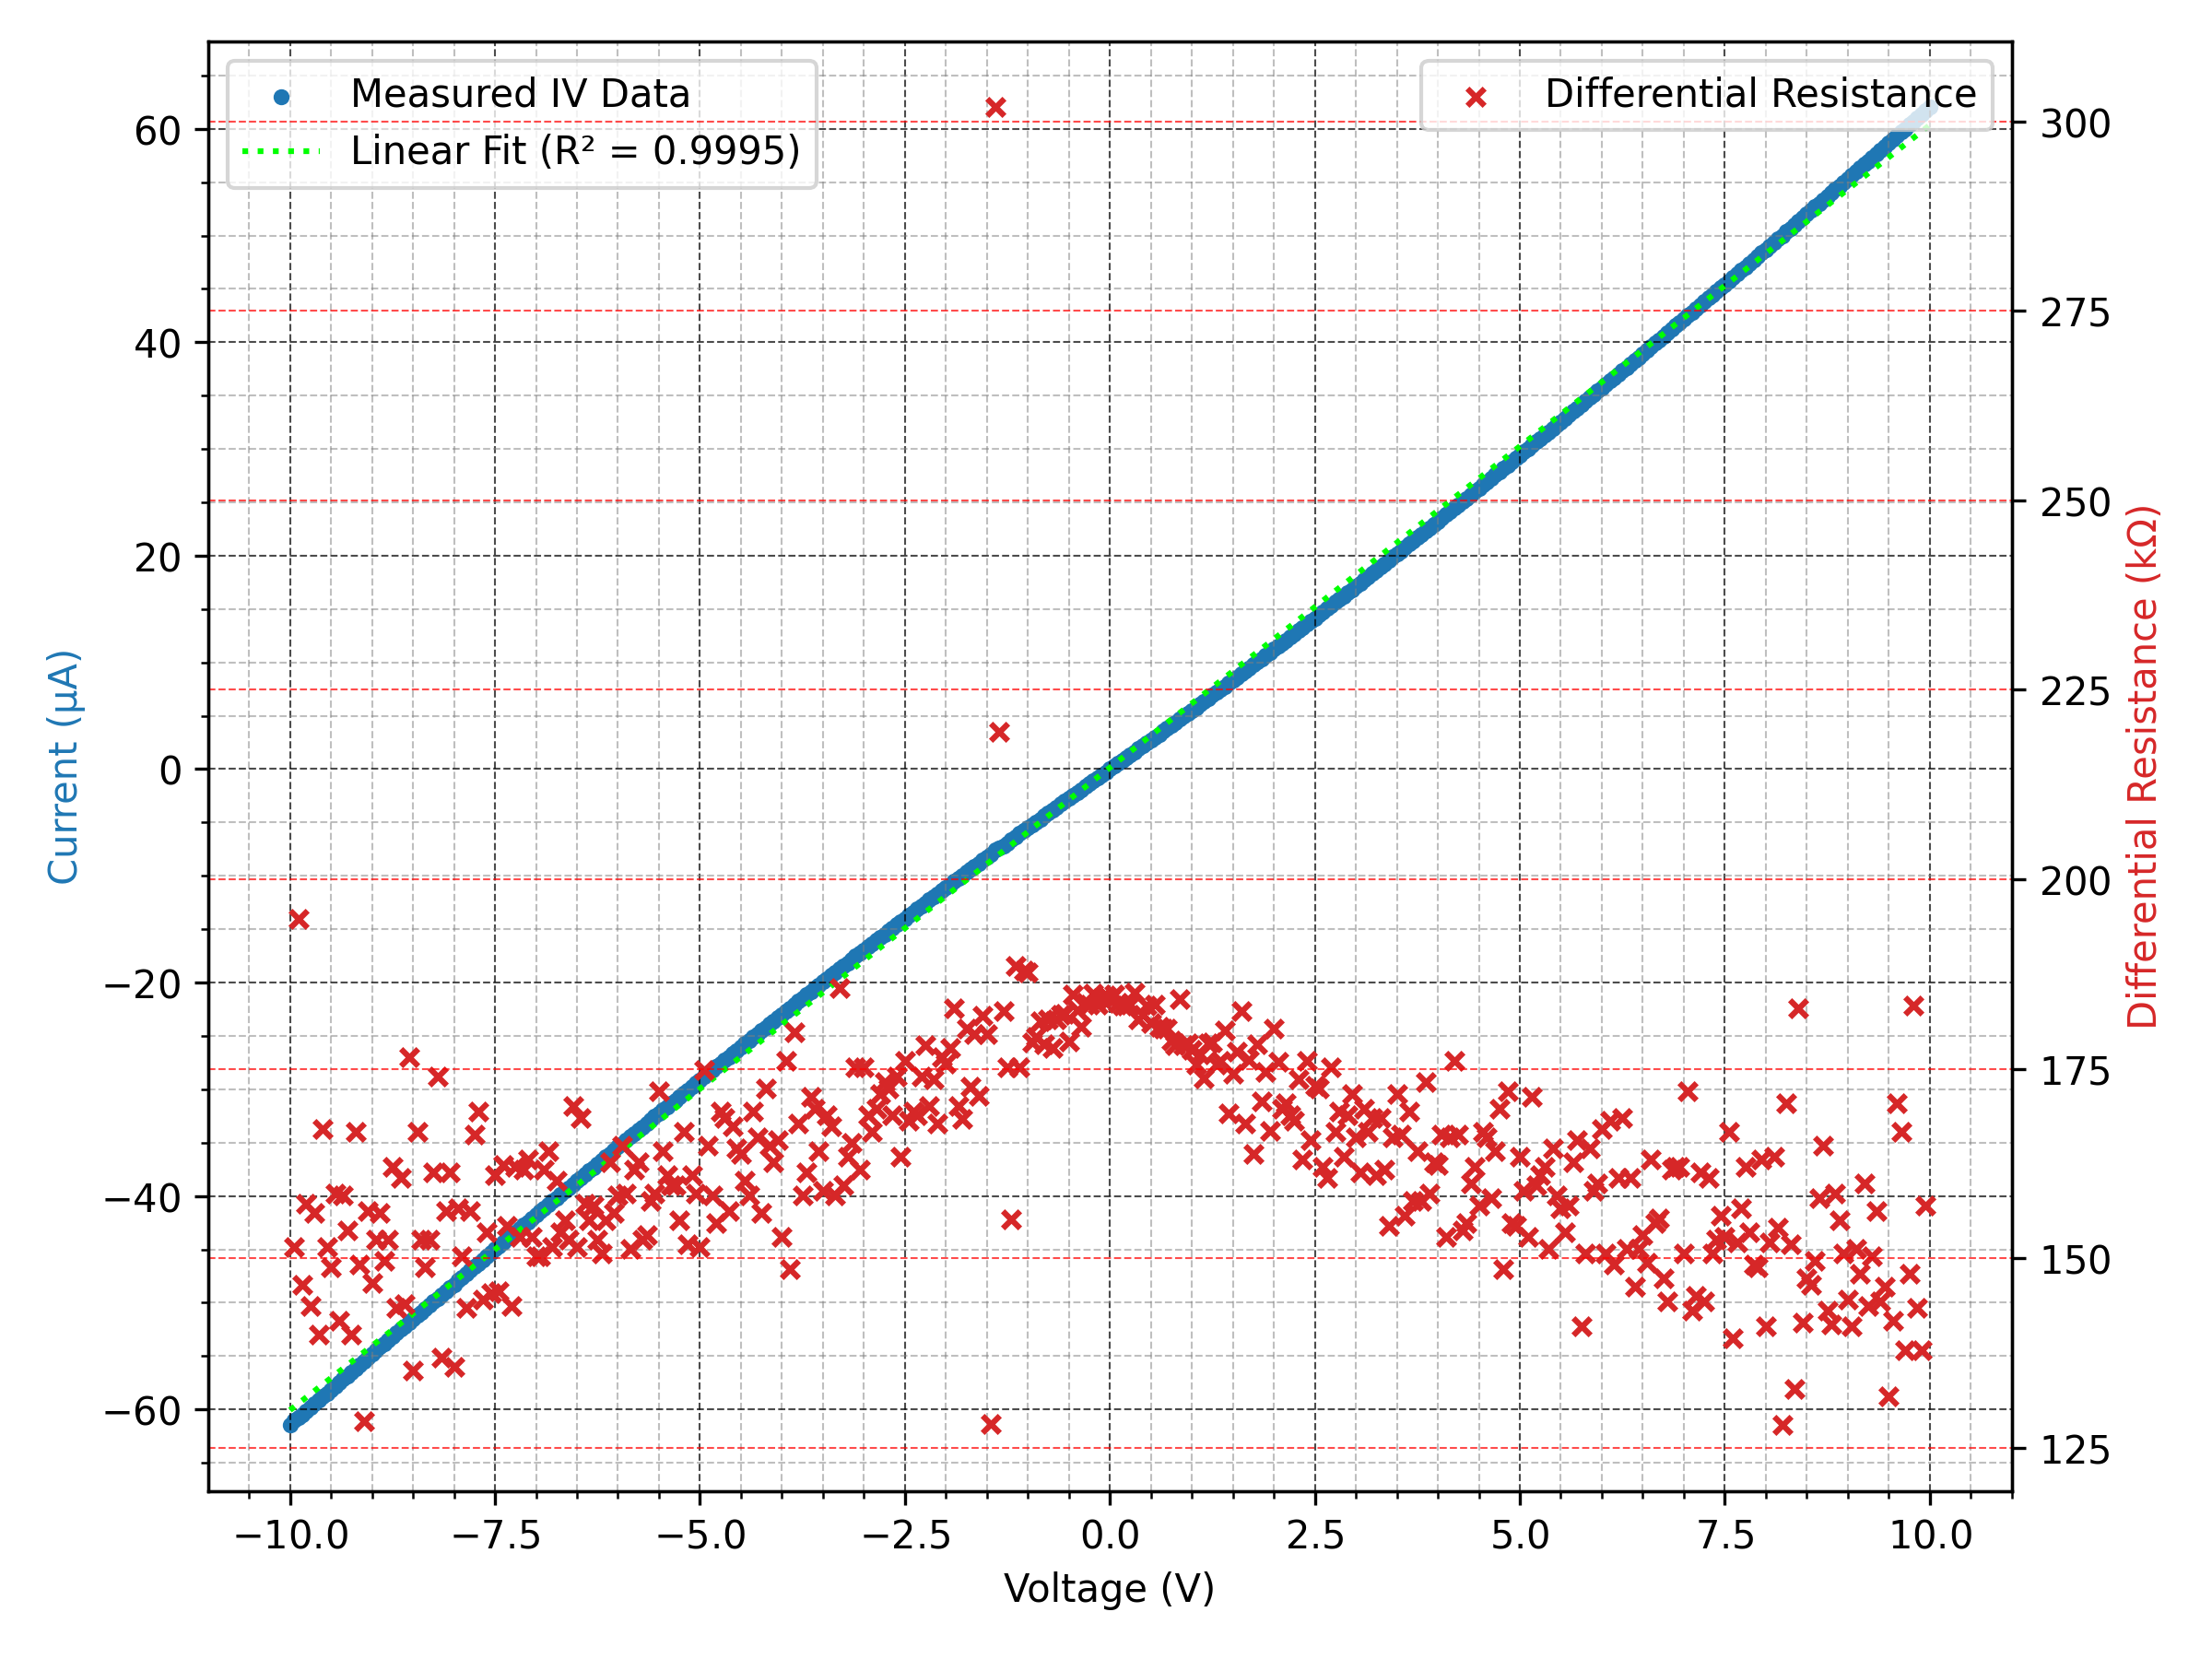
\includegraphics[width=\linewidth]{Chapter7/Figs/Raster/Emitters/43 3x 10V.png}
    \caption{The average electrical characteristics between probe positions 4 and 3.}
    \label{fig:e_43_10v}
\end{figure}

\begin{table}[h!]
\centering
\begin{tabular}{|c|c|c|c|c|}
\hline
\textbf{Voltage (V)} & \textbf{Resistance (\si{\mega\ohm})}  & \textbf{Resistivity (\si{\ohm\centi\metre})} & \textbf{Conductivity (\si{\siemens\per\metre})} \\
\hline
10 & $0.166$ & $2.08$ & 48.2 \\
\hline
\end{tabular}
\caption{Extracted wire parameters for wire 4-3, $\pm10$~\si{\volt} measurements.}
\label{tab:43_e_wire_parameters_10v}
\end{table}

Figure \ref{fig:e_43_10v} shows the electrical characteristics as measured with probe positions 4-3 on the top of contact C. This essentially a measurement of the wire at the top of contact C. 401 data points across 3 separate $\pm10$~\si{\volt} sweeps, with assumptions as used in the characterisation of trial wires in section \ref{subsec:testing_of_surface_graphitic_wires} are used to provide estimated wire properties as summarised in table \ref{tab:43_e_wire_parameters_10v}.

\subsection{Low-Voltage Wire Testing: 2-1}
\begin{figure}[H]
    \centering
    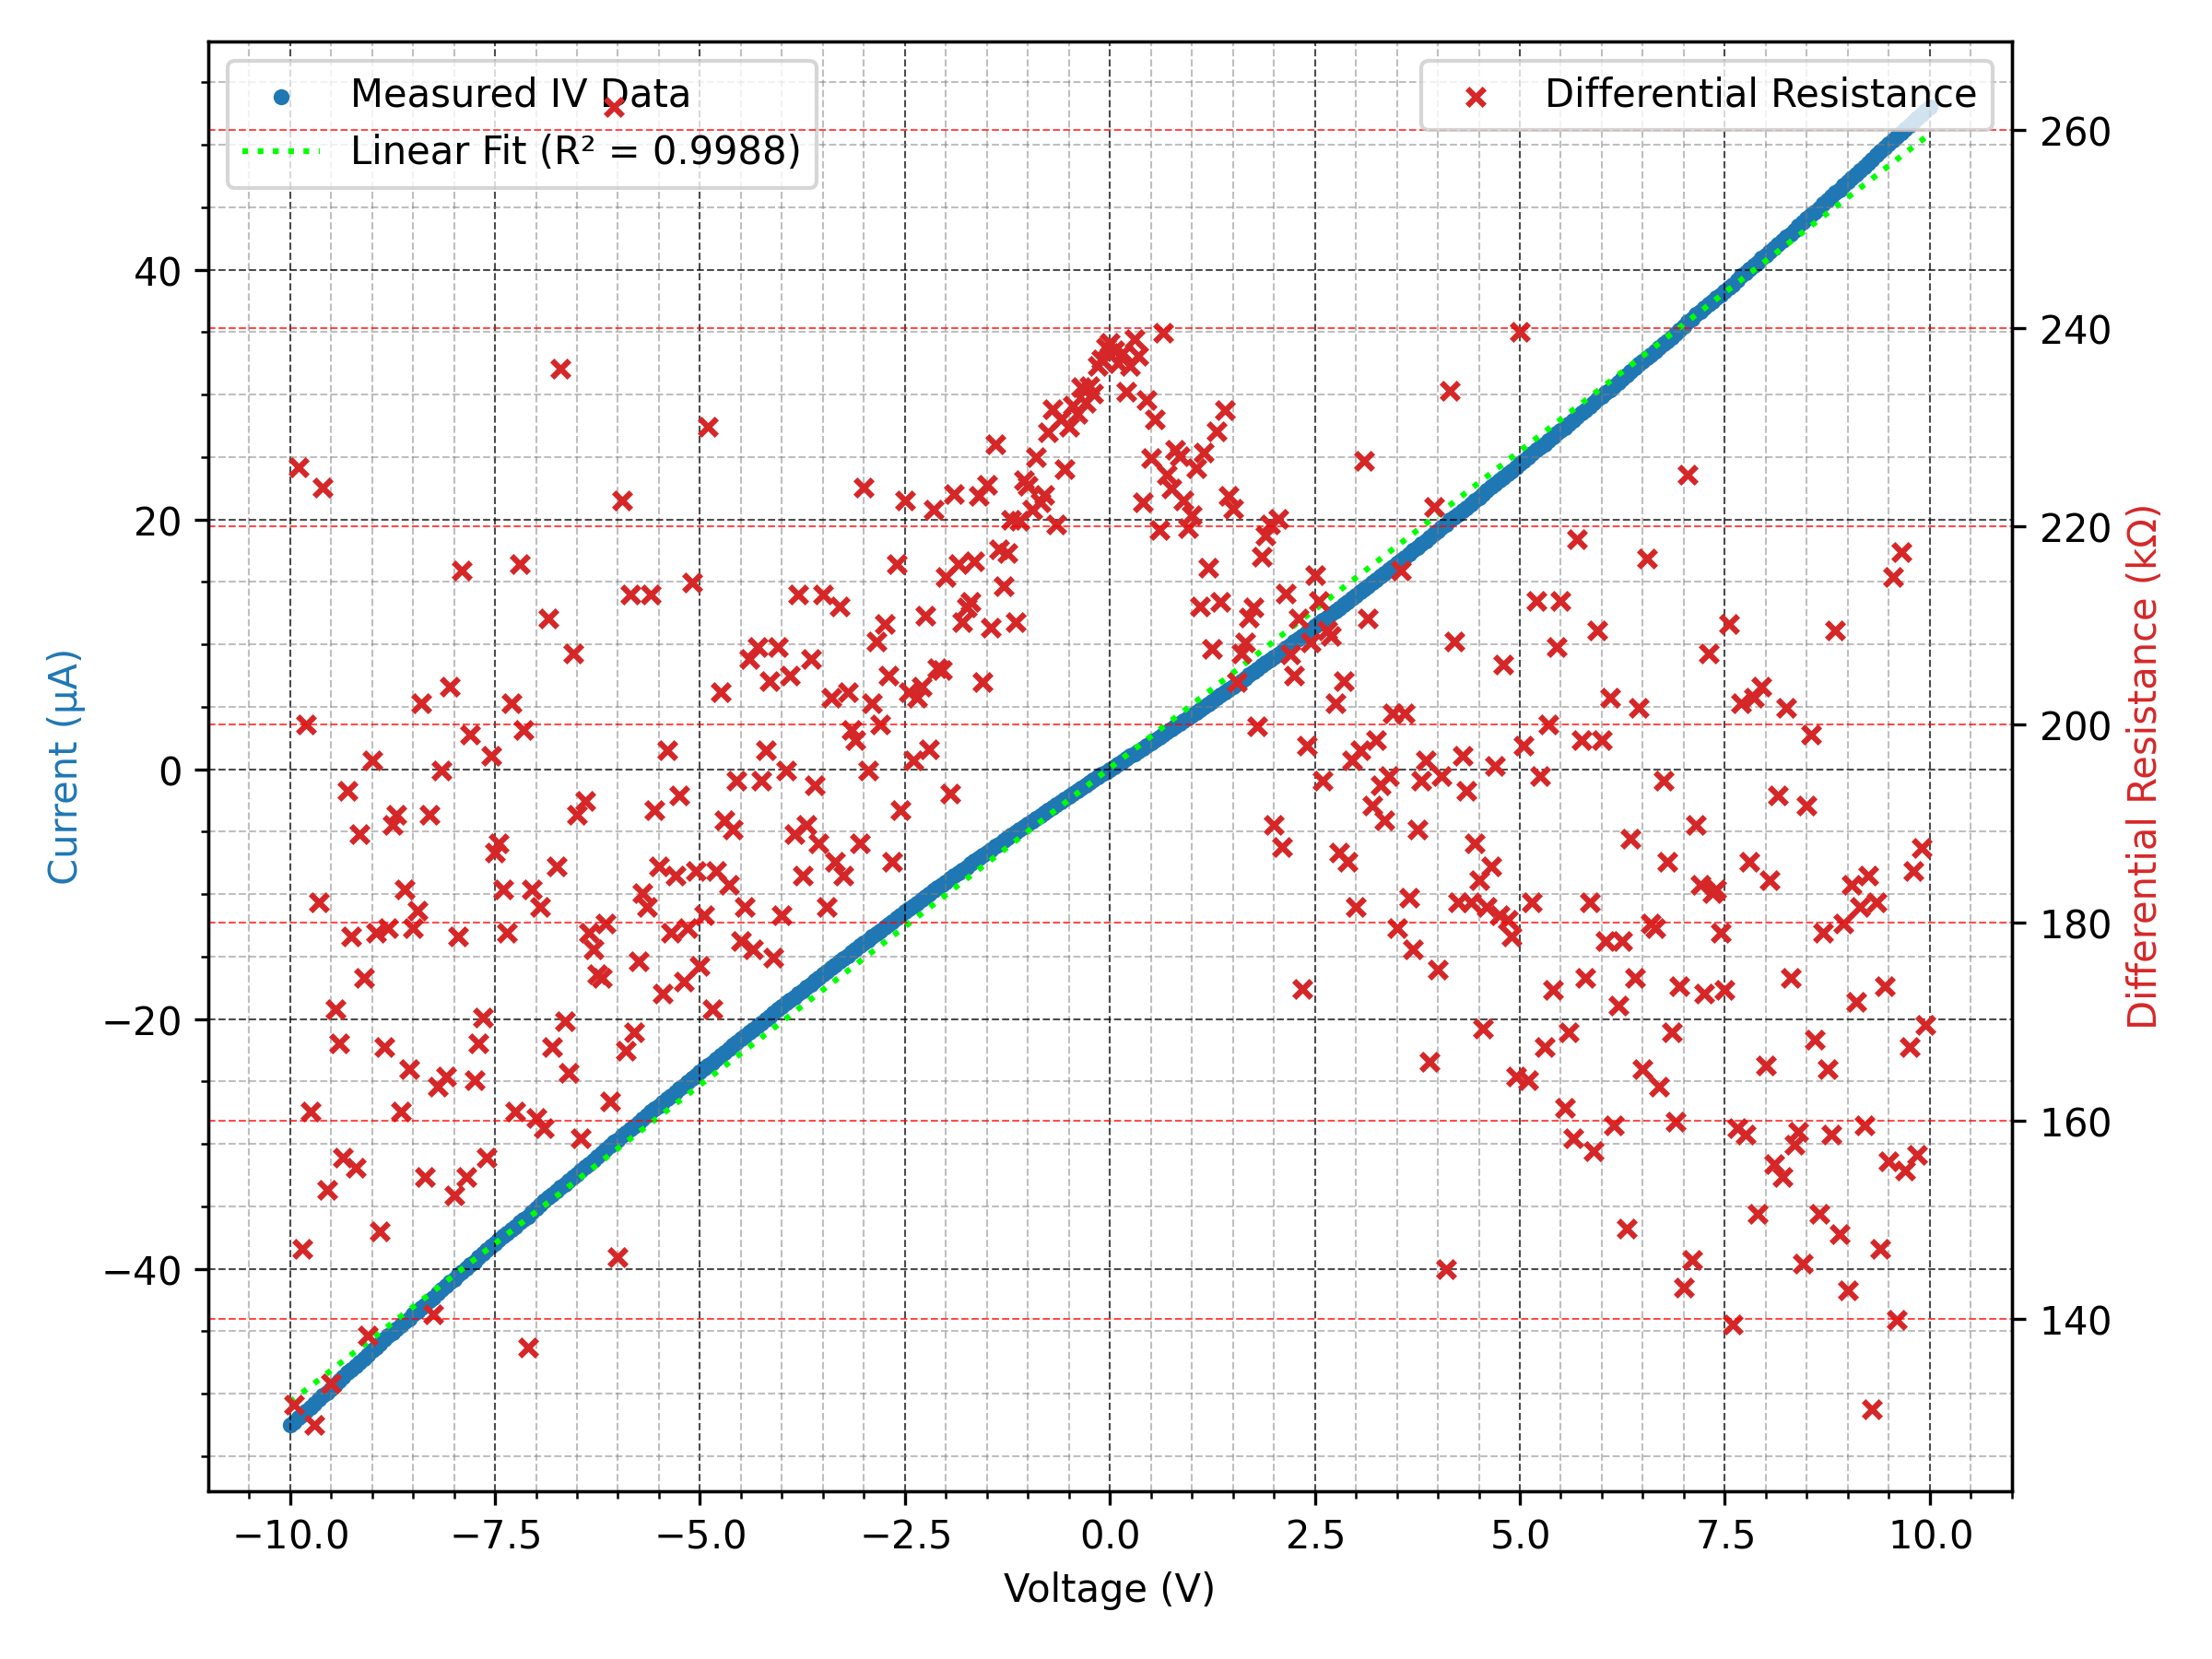
\includegraphics[width=\linewidth]{Chapter7/Figs/Raster/Emitters/21 3x 10V.png}
    \caption{The average electrical characteristics between probe positions 2 and 1.}
    \label{fig:e_21_10v}
\end{figure}

\begin{table}[h!]
\centering
\begin{tabular}{|c|c|c|c|c|}
\hline
\textbf{Voltage (V)} & \textbf{Resistance (\si{\mega\ohm})}  & \textbf{Resistivity (\si{\ohm\centi\metre})} & \textbf{Conductivity (\si{\siemens\per\metre})} \\
\hline
10 & $0.197$ & $2.46$ & 40.6 \\
\hline
\end{tabular}
\caption{Extracted wire parameters for wire 2-1, $\pm10$~\si{\volt} measurements.}
\label{tab:21_e_wire_parameters_10v}
\end{table}

Figure \ref{fig:e_21_10v} provides the electrical characteristics for the wire between probe positions 2-1 on contact H. The extracted parameters are summarised in table \ref{tab:21_e_wire_parameters_10v}. This wire shows a slightly higher effective resistivity than the wire between 4-3, but is otherwise reasonably similar in properties. Both wires are an order of magnitude lower in conductivity than the 10~\si{\micro\metre} wires tested in section \ref{subsubsec:graphitised_wire_testing_10}, which indicates some local variation in the diamond substrate or laser writing affecting the wires between these two regions. The differential resistance in figure \ref{fig:e_21_10v} is notably scattered over a wider range of values than that of figure \ref{fig:e_43_10v}, but again the rise in resistance around a bias of 0~\si{\volt} is not as pronounced as in the case of data with a clear Schottky behaviour, and the scatter only shows a slight deviation from ohmic behaviour for these wires.

\subsection{Low-Voltage Emitter Testing: 4-2}
Before switching the probe positions to that of a-b, measurements were taken with the 4 probe positions as for the wire testing, which provides a first look at the IV characteristics of this emitter array.
\begin{figure}[H]
    \centering
    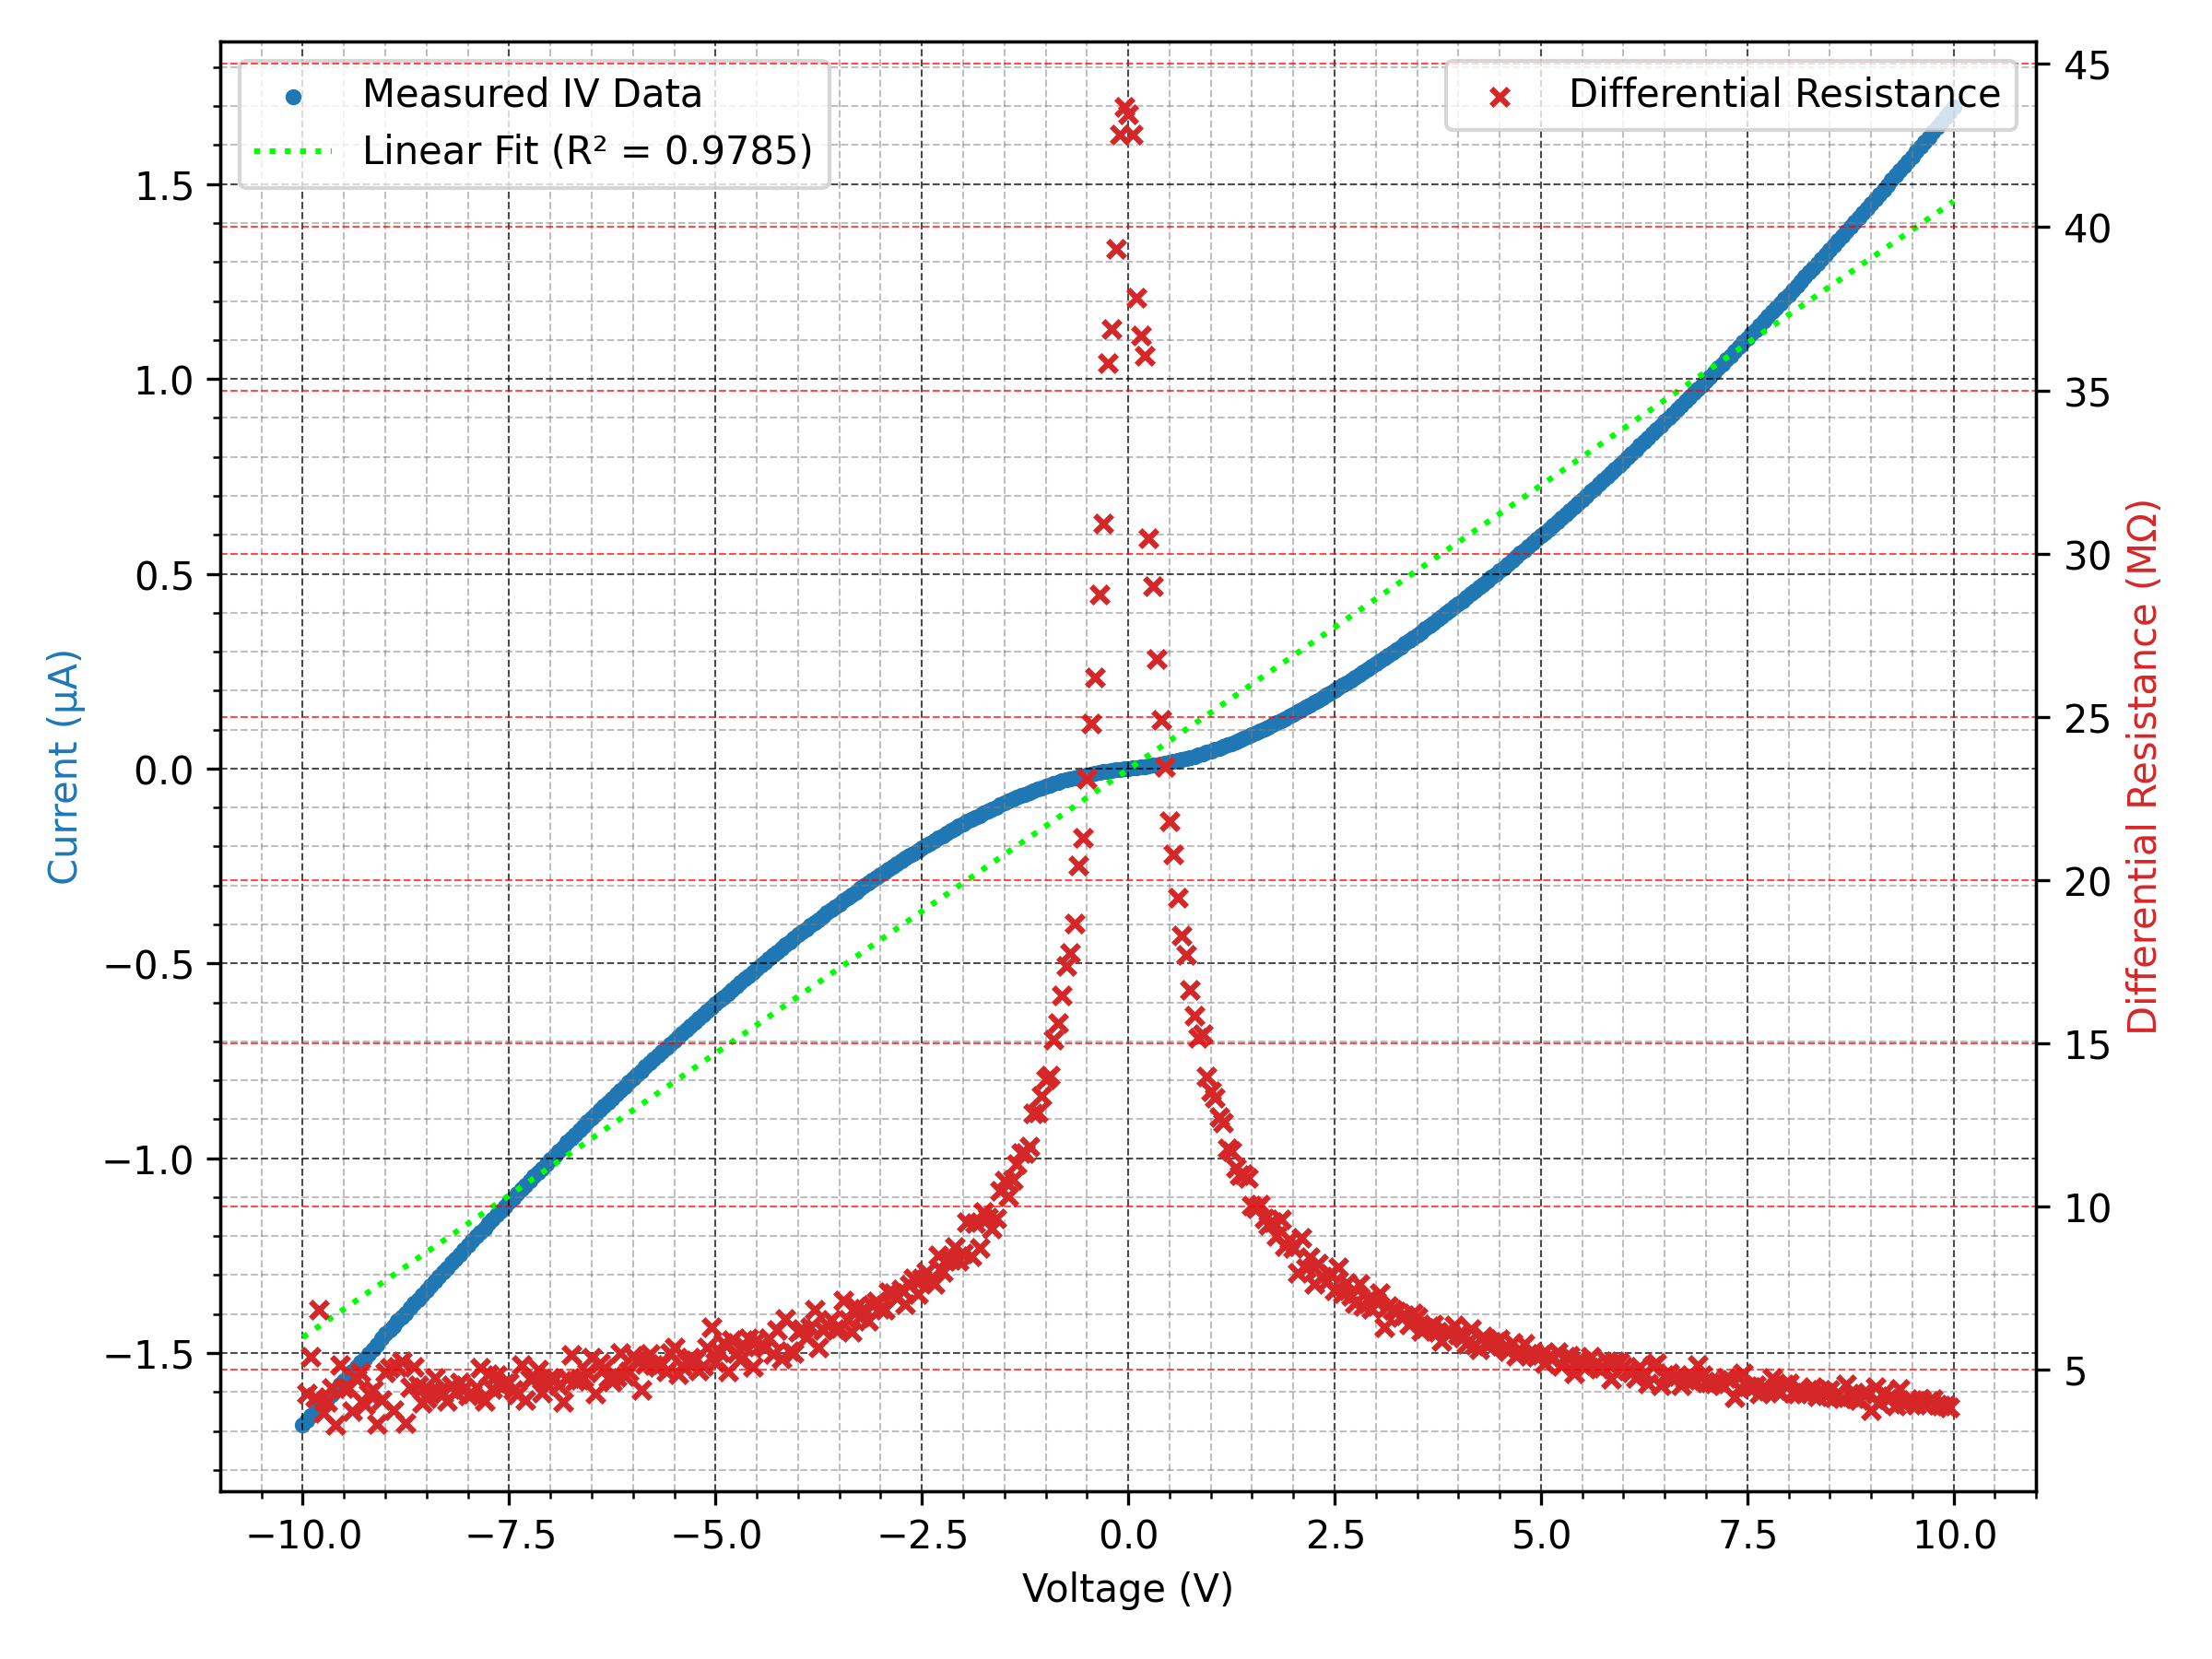
\includegraphics[width=\linewidth]{Chapter7/Figs/Raster/Emitters/42 3x 10V.png}
    \caption{The average electrical characteristics between probe positions 4 and 2.}
    \label{fig:e_42_10v}
\end{figure}

\begin{table}[h!]
\centering
\begin{tabular}{|c|c|c|c|c|}
\hline
\textbf{Voltage (V)} & \textbf{Resistance (\si{\mega\ohm})}  & \textbf{Resistivity (\si{\ohm\centi\metre})} & \textbf{Conductivity (\si{\siemens\per\metre})} \\
\hline
10 & $6.86$ & $85.7$ & 1.17 \\
\hline
\end{tabular}
\caption{Extracted wire parameters for "wire" approximation of 4-2, $\pm10$~\si{\volt} measurements.}
\label{tab:42_e_wire_parameters_10v}
\end{table}

Figure \ref{fig:e_42_10v} presents the low voltage measurements taken across probe positions 4-2, with table \ref{tab:42_e_wire_parameters_10v} providing estimated values for the resistivity using the 10~\si{\micro\metre} wire approximation for direct comparison to previous results. This approximation is useful for comparing orders of magnitude, but since the channel resistivity will be the dominant factor, the wire dimensions approximation merely shows that the electrical data reflect the emitter channel under testing. The IV characteristics here resemble those of the LTLM channels tested in section \ref{subsec:ltlm2_lost_data}, which is a reassuring comparison, as at this potential bias the expected maximum electric field norm on emitter tips is of the order of $10^{5}$~\si{\volt\per\metre}. Hence, with a low applied potential difference, the expectation is for the measured current to be due to thermionic emission. Further simulations examining the expected balance between thermal and field effect emission processes are presented in section \ref{sec:modelling}.

\subsection{Low-Voltage Emitter Testing: a-b Ramp-Up}
With the conductivities of laser written contact wires established in the $40$--$48$~\si{\siemens\per\metre} region, electrical characterisation was undertaken with the probes placed as closely as possible to the middle of the far sides of the contacts, as indicated by positions a and b in figure \ref{fig:emitter_esid_anno}. This was chosen to ensure that the distances between probes and the emitter channel were close to identical on either side of the contact structures, hence presenting the best chance of all 10 emitter wires participating in the flow of current across contacts C-H. Brief electrical checks were performed with an additional probe on adjacent contact structures to ensure that the path of least resistance was indeed the emitter channel between C-H. This can be justified with the general observation via optical microscopy that no direct laser processed wires link either contact to any of the adjacent contacts, instead, there are 3 emitter channels of similar spacing as between C-H. The brief electrical checks ensured that all of these emitter channels had a similar level of current flow at low voltage, and so it is possible to focus entirely on the channel between contact C and H in these measurements.

\begin{figure}[H]
    \centering
    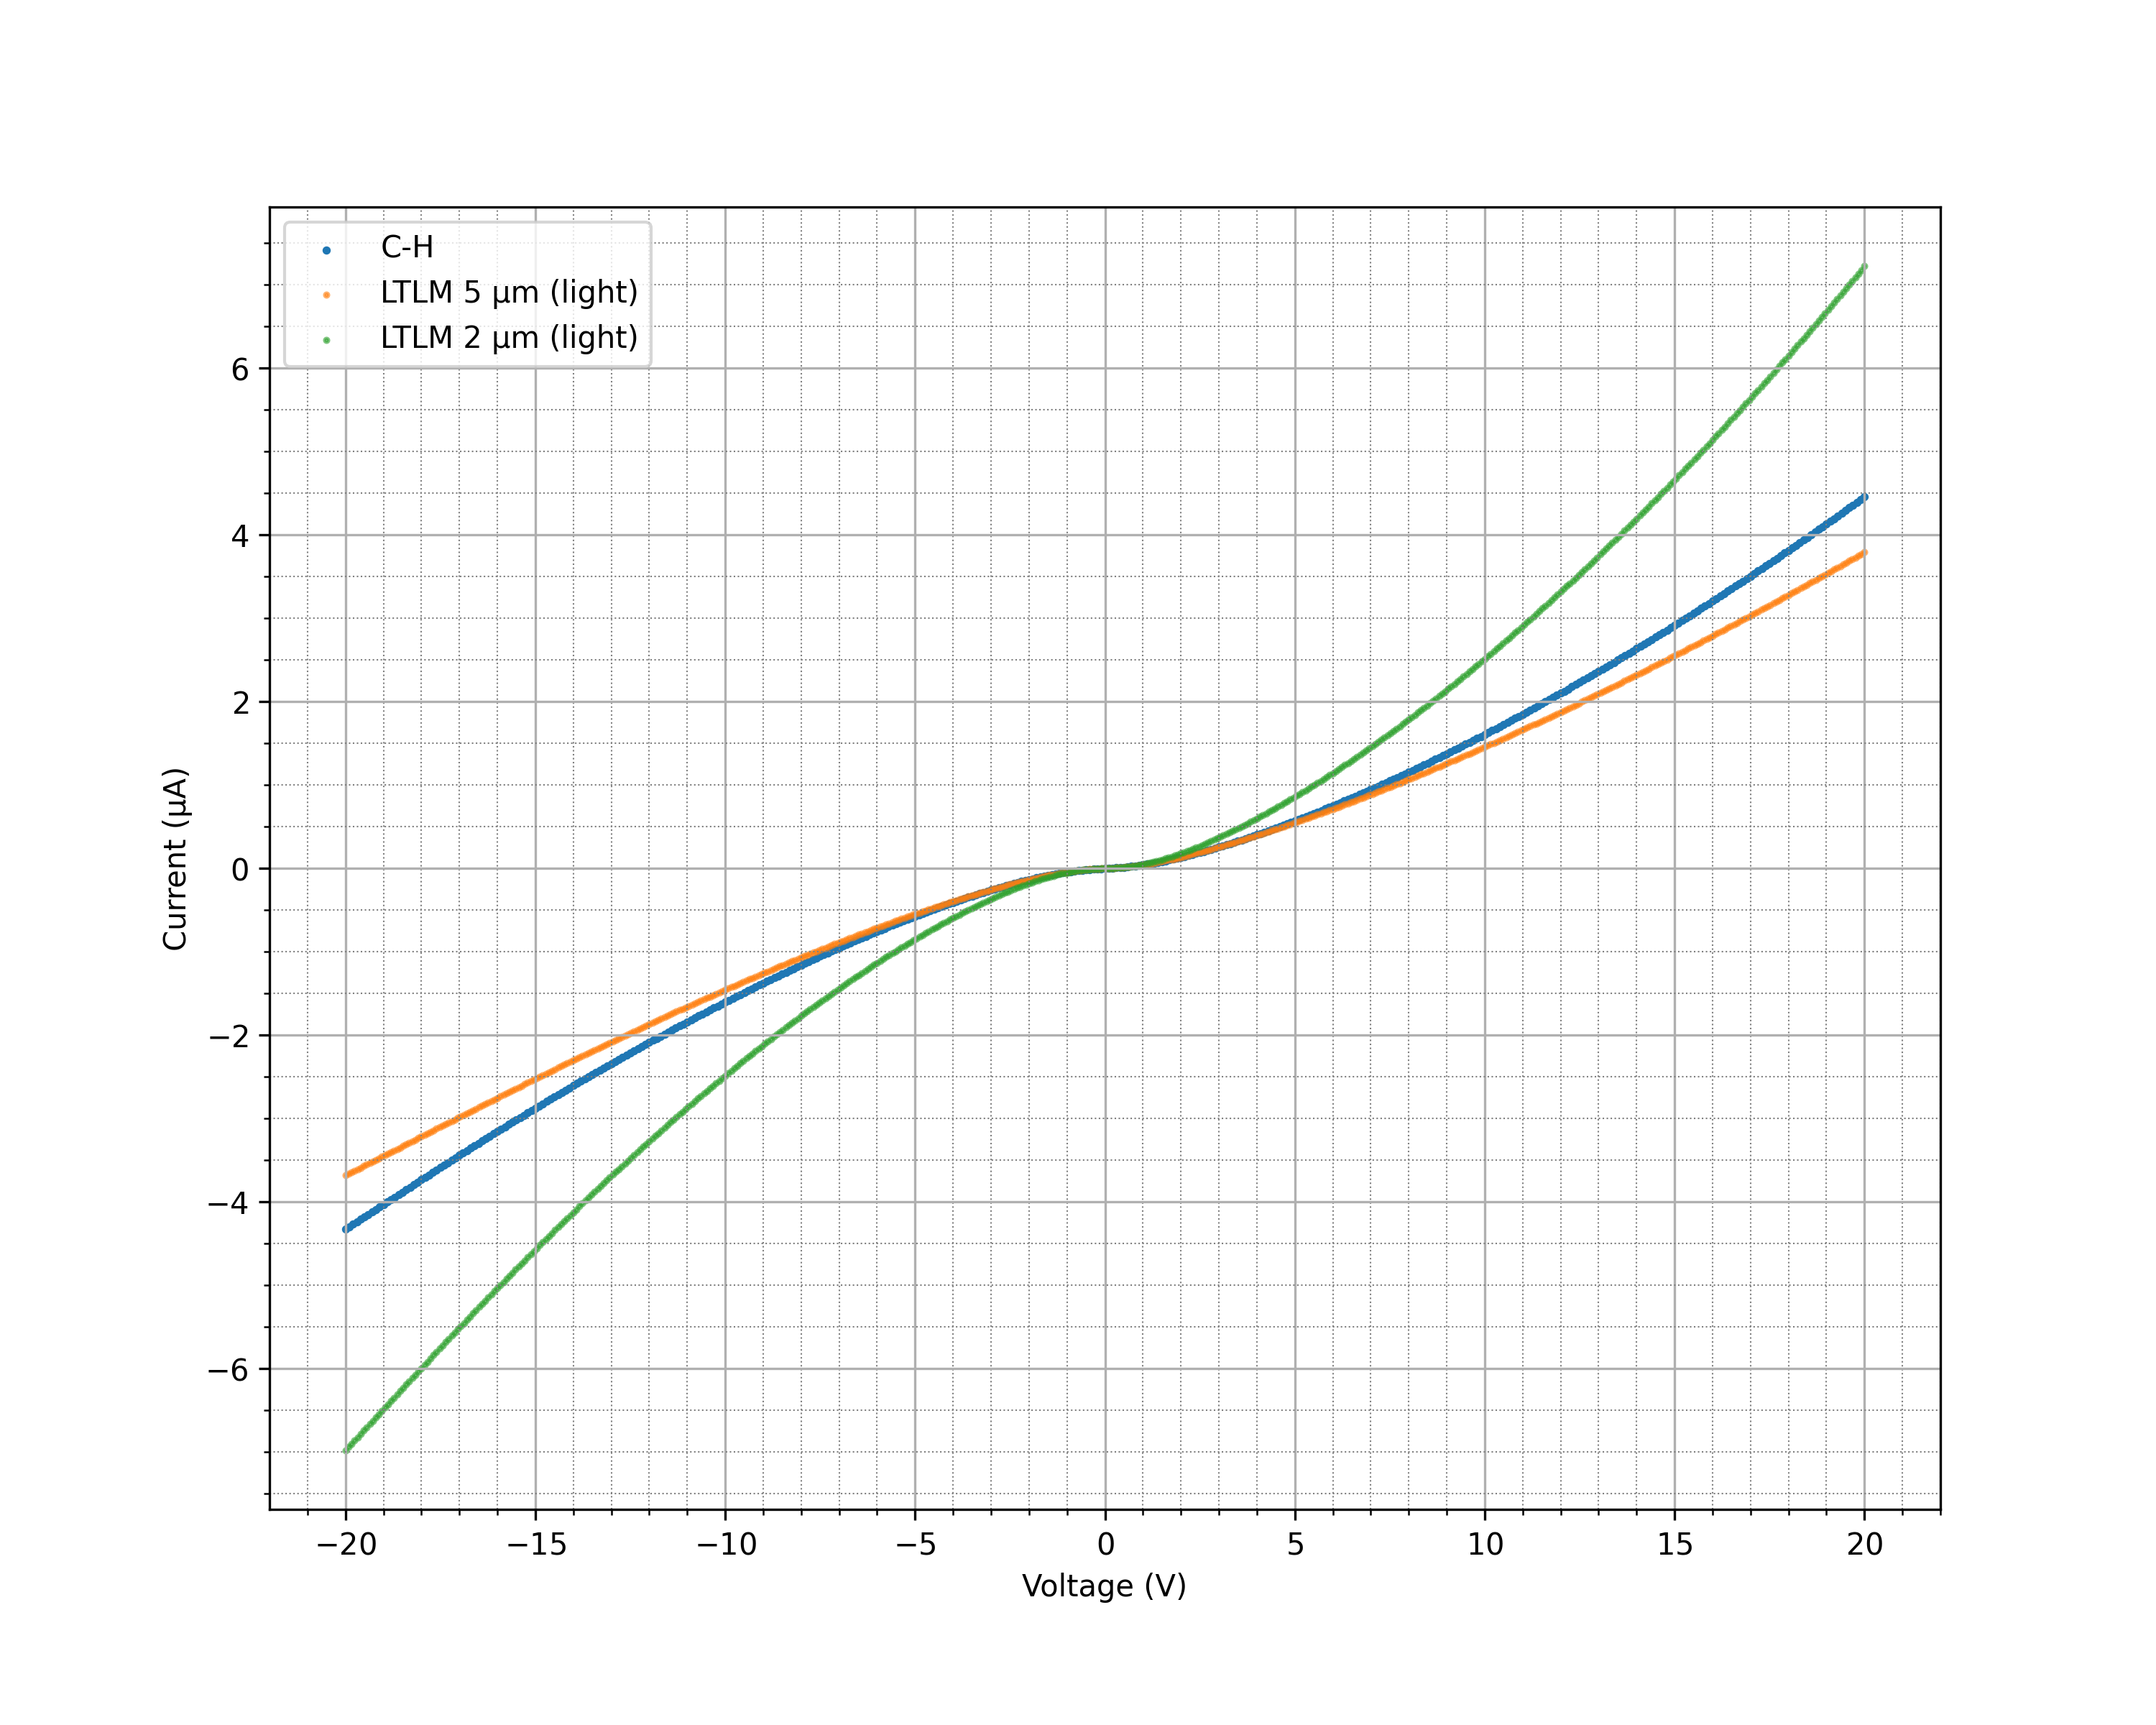
\includegraphics[width=\linewidth]{Chapter7/Figs/Raster/Emitters/20V comparison to LTLM.png}
    \caption{The average electrical characteristics between probes a-b representing emitter structure CH, compared to LTLM measurements across 2 and 5~\si{\micro\metre} channels.}
    \label{fig:e_ch_20v_ltlm}
\end{figure}

Figure \ref{fig:e_ch_20v_ltlm} shows and compares the 20~\si{\volt} IV characteristics of emitter channel CH to those of the two comparable LTLM channels. CH may be described as a 5~\si{\micro\metre} LTLM channel, with the addition of 10 small emitter wires of length 2.5~\si{\micro\metre}, reducing the actual channel length by half. Optical characterisation of the 2~\si{\micro\metre} LTLM channel revealed that the effective spacing for that structure may be slightly lower, so it is quite natural to see that in this voltage range, the CH channel presents a slightly lower resistance than the 5~\si{\micro\metre} LTLM channel, but a significantly higher resistance than the 2~\si{\micro\metre} channel. Note that in the case of emitter testing, all electrical characterisation was performed under direct illumination, hence the LTLM characteristics taken in complete darkness seen in section \ref{subsec:ltlm2_lost_data} are not used in this comparison.

\begin{figure}[H]
    \centering
    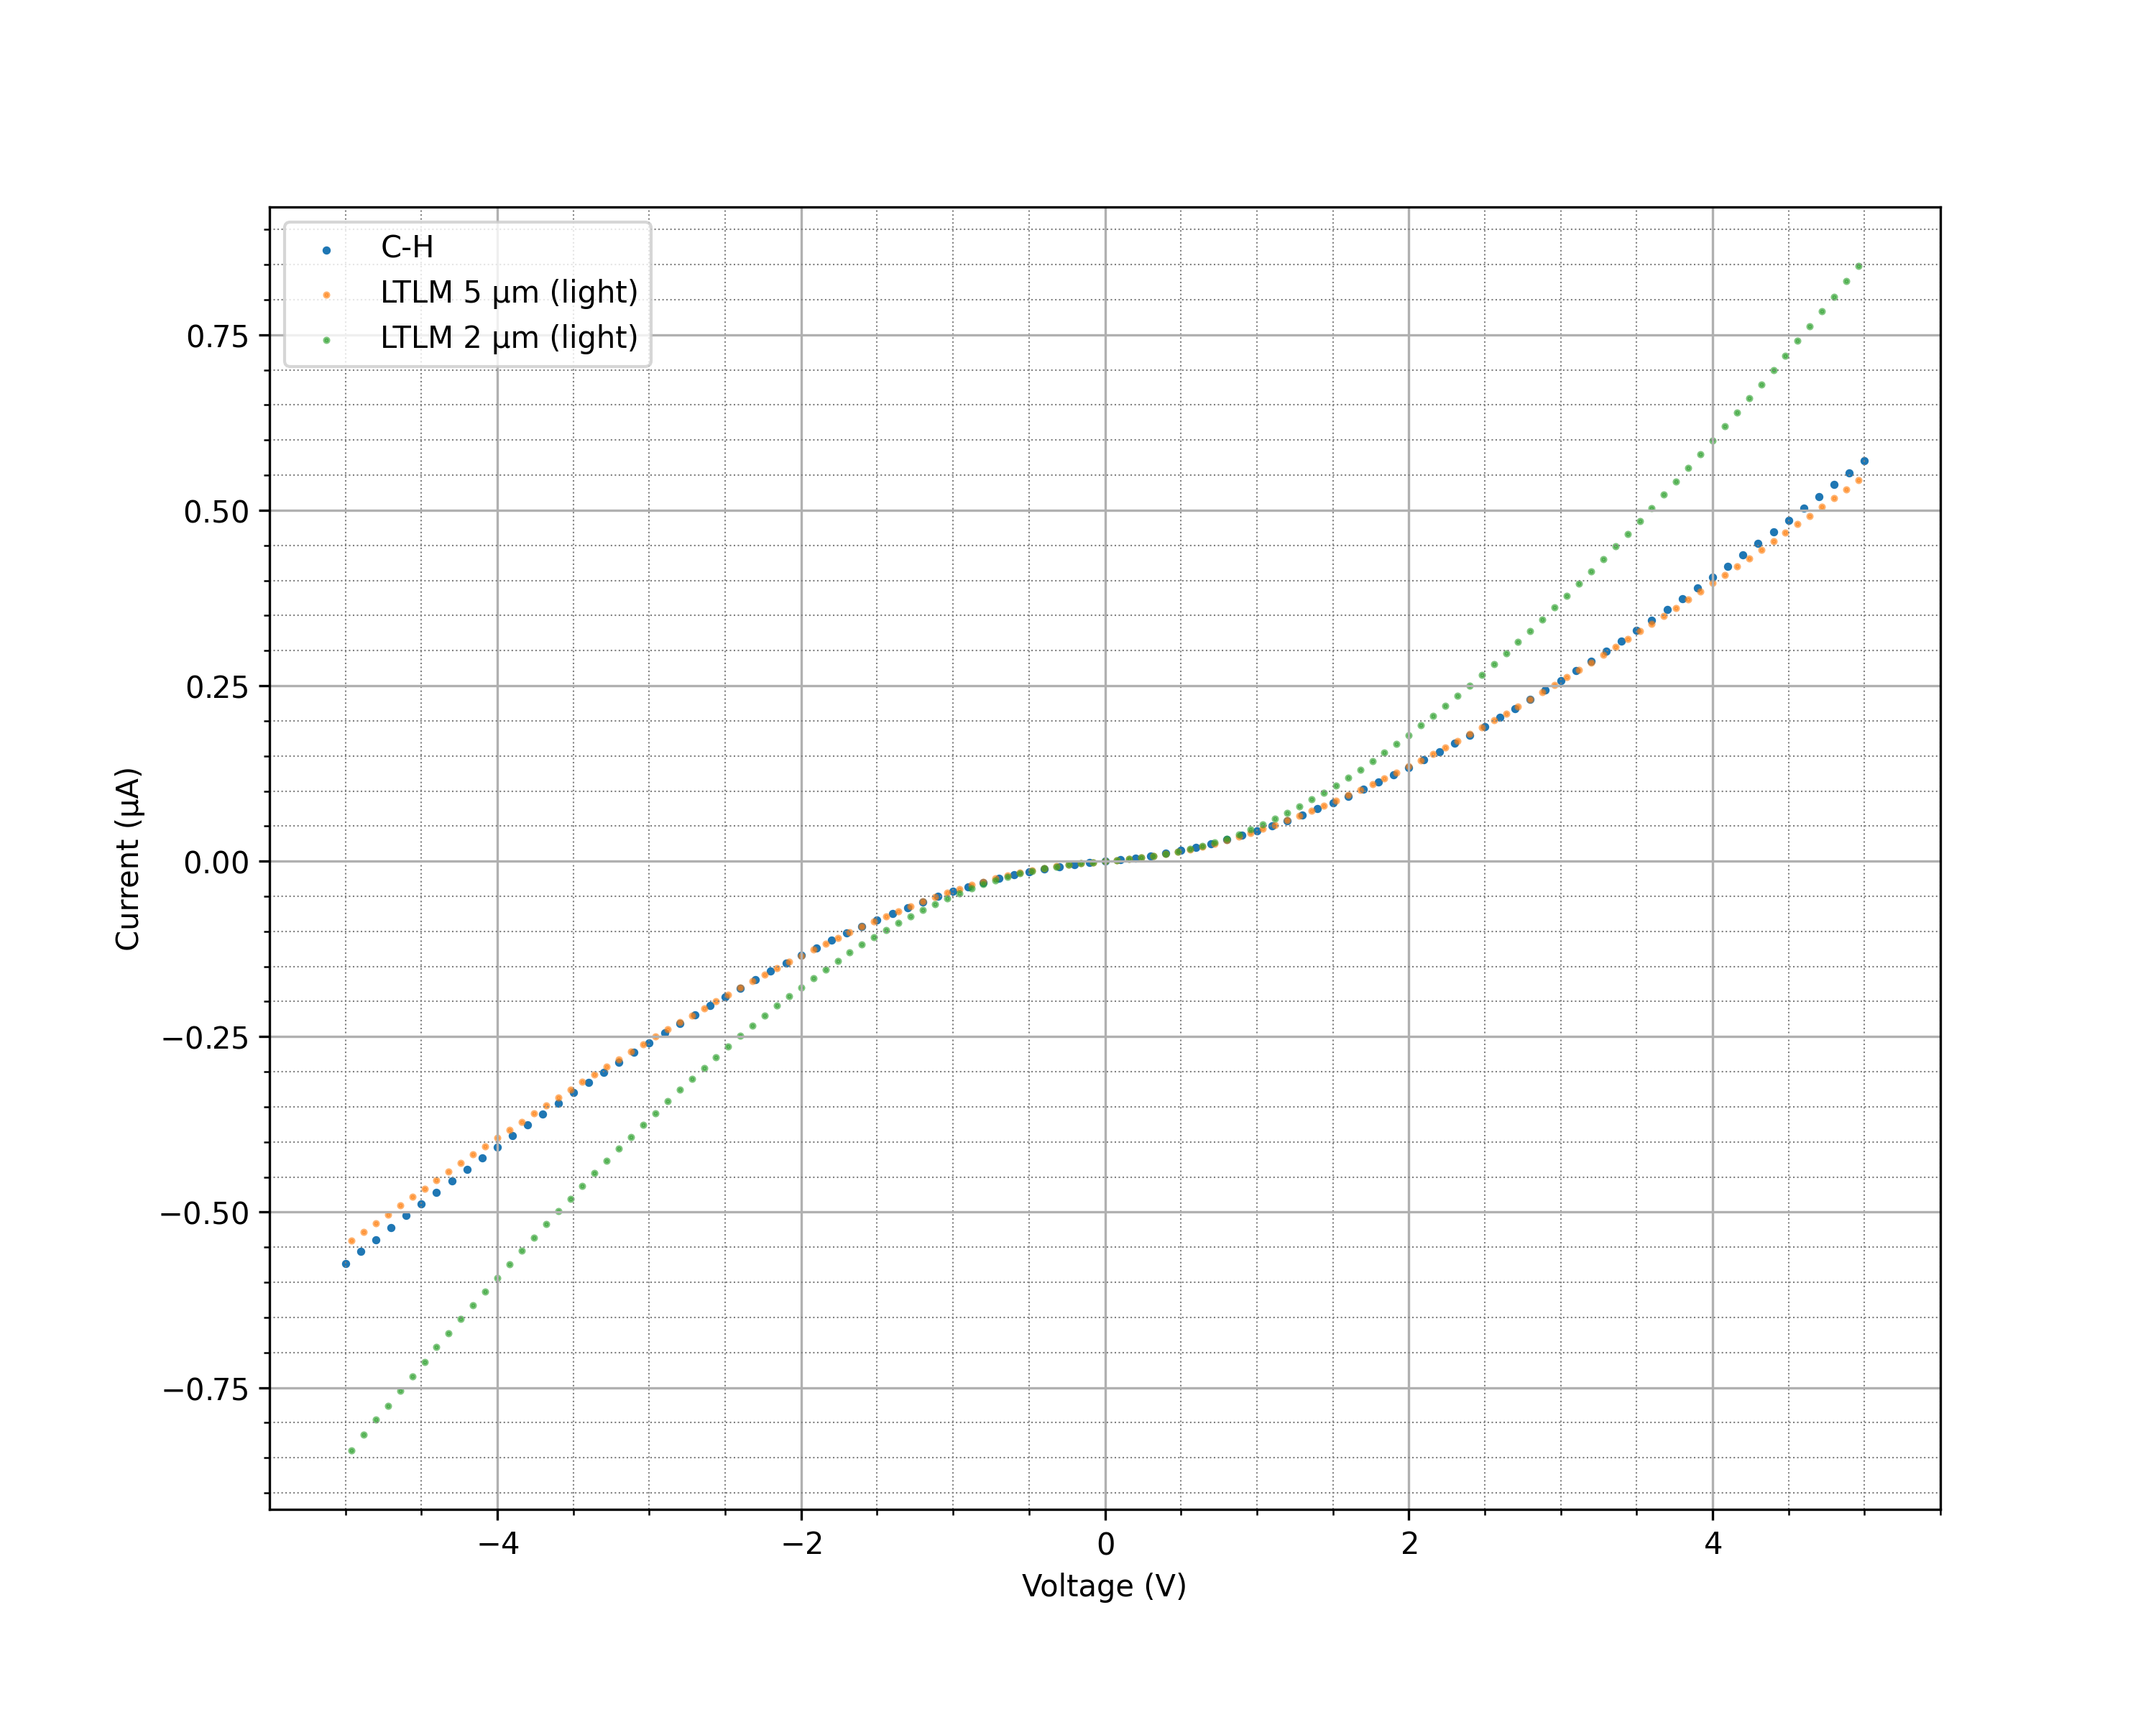
\includegraphics[width=\linewidth]{Chapter7/Figs/Raster/Emitters/5V comparison to LTLM.png}
    \caption{The average electrical characteristics between probes a-b representing emitter structure CH, compared to LTLM measurements across 2 and 5~\si{\micro\metre} channels.}
    \label{fig:e_ch_5v_ltlm}
\end{figure}

Figure \ref{fig:e_ch_5v_ltlm} provides a closer look at the low voltage region of emitter CH, alongside the comparable LTLM data. Again, the CH data closely resembles that of the LTLM structures in this voltage region, presenting as though this is another LTLM channel with a double Schottky structure making use of thermionic emission across a channel length between 2 and 5~\si{\micro\metre}. It is particularly similar to the 5~\si{\micro\metre} data in this comparison, perhaps indicating that the thin emitter wires have a significantly higher resistivity.

\subsection{High-Voltage Emitter Testing: a-b Ramp-Up}
Following confirmation that at low potential differences the CH emitter structure is dominated by thermionic emission, and is very similar to that of the 5~\si{\micro\metre} LTLM structure, higher voltage testing to reach normal electric fields suitable for Fowler-Nordheim type field effect emission proceeded with the bias region increasing from $\pm5$ to $120$~\si{\volt}, mostly in 10~\si{\volt} intervals. All measurements are performed with contact C (the emitter array) held at ground and a potential bias is applied to contact H (anode).

\begin{figure}[H]
    \centering
    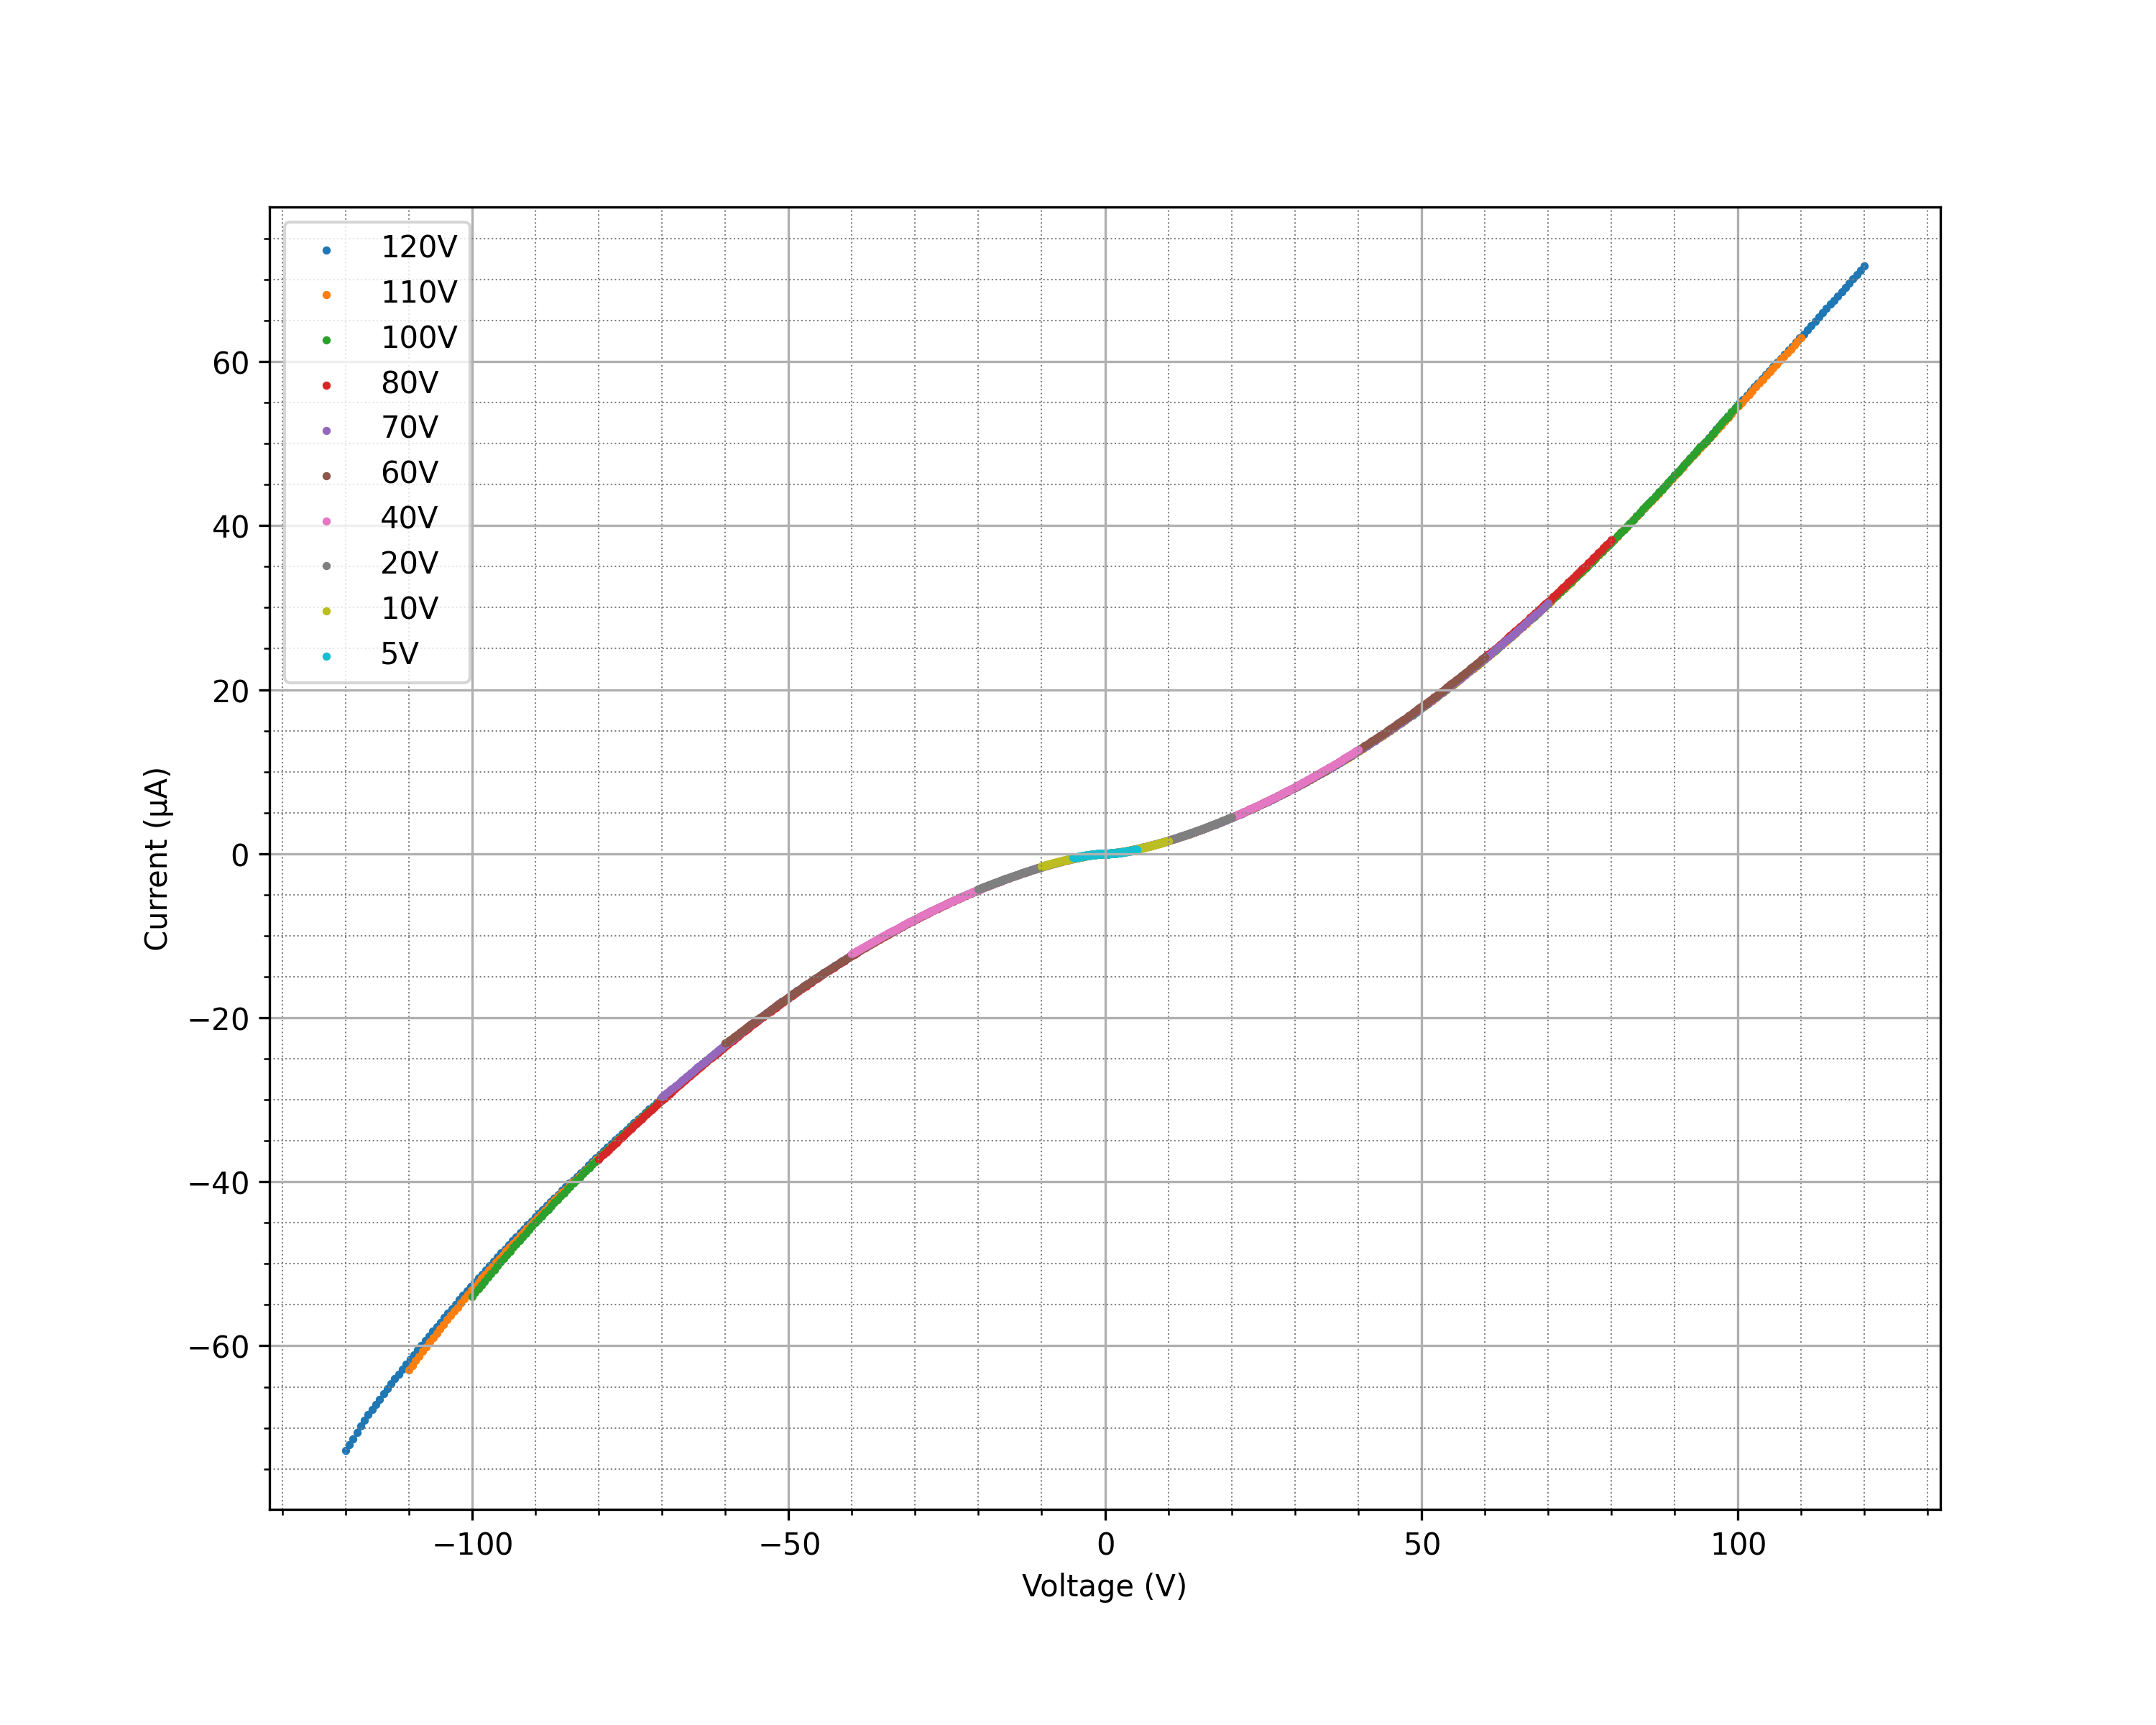
\includegraphics[width=\linewidth]{Chapter7/Figs/Raster/Emitters/5-120V sweeps.png}
    \caption{The average electrical characteristics between probes a-b representing emitter structure CH, from 5--120~\si{\volt}}
    \label{fig:e_ch_5-120v_iv}
\end{figure}

Figure \ref{fig:e_ch_5-120v_iv} presents a summary of the ramping up of voltage that was performed with emitter structure CH. The scatter points are overlaid from the highest bias sweep characteristics to the lowest bias sweep, to allow the closely overlapping scatter points to be distinctly visible from one another. At the higher voltages, a slight asymmetry begins to present itself, deviating from the standard double Schottky IV characteristic, however this is difficult to observe from IV characteristics.

\begin{figure}[H]
    \centering
    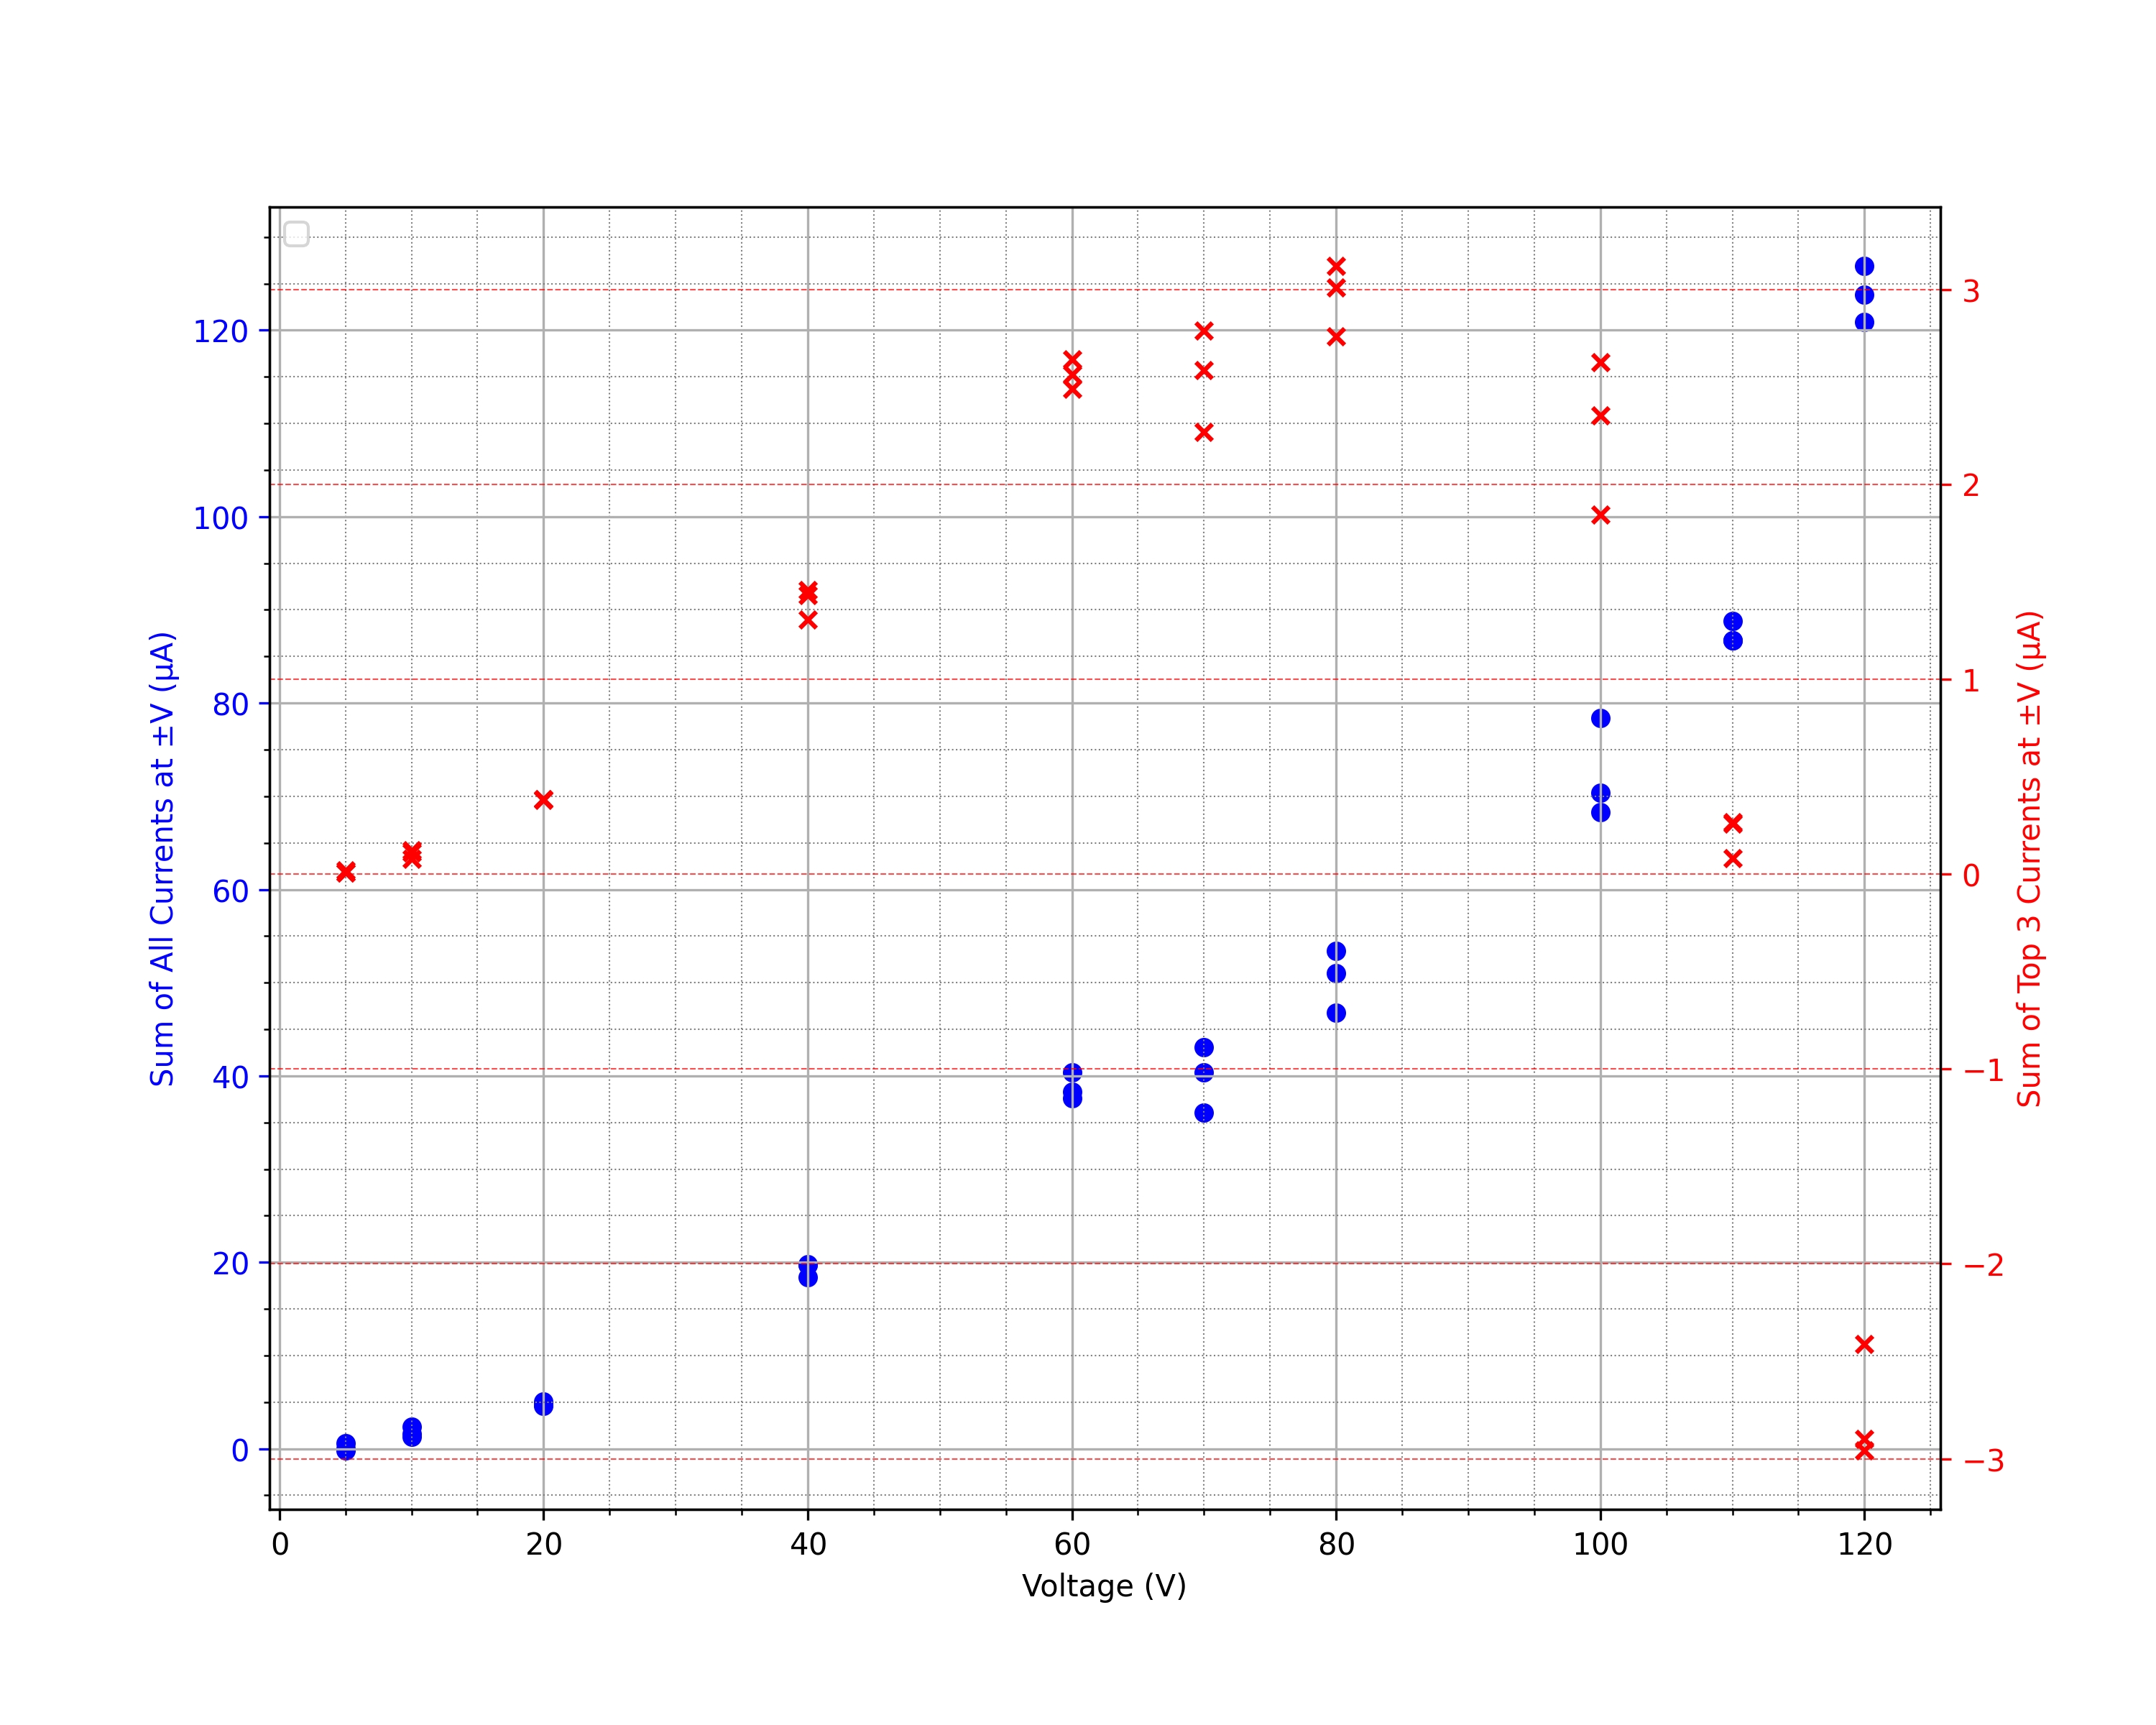
\includegraphics[width=\linewidth]{Chapter7/Figs/Raster/Emitters/5-120V asymmetry.png}
    \caption{The total and peak asymmetry for emitter CH from 5--120~\si{\volt}}
    \label{fig:e_ch_5-120v_asymmetry}
\end{figure}

In figure \ref{fig:e_ch_5-120v_asymmetry}, the asymmetry observed in the IV characteristics is quantified in two ways. On the left axis (blue scatter), the sum of all currents measured is plotted. In an ideal ohmic resistor, this value should be 0, as the magnitude of current drawn in forward bias is no different to that of the current in reverse bias, and the sum of positive and negative currents will be zero. Equally, with symmetric back to back Schottky contacts, it is expected that there is no preference for the direction in current. Differences are due to differing ideality factors or barrier heights between the two Schottky junctions, but in this case it is expected that at high voltage a field effect emission current will be present. Hence, asymmetry due to the total current sum may help identify field effect emission contributions to current flow.

It was noted during the experimental process that the asymmetry was particularly pronounced at the absolute maximum and minimum potential biases. The right axis (red scatter) presents the sum of the 3 highest and 3 lowest measured currents, giving an indication of asymmetrical peak current. The sum of all currents in figure \ref{fig:e_ch_5-120v_asymmetry} tends to increase for higher voltages, indicating an overall asymmetry in the positive bias direction. In contrast, while in agreement to begin with, the sum of the peak 3 currents rises to an asymmetry of 3~\si{\micro\ampere} at 80~\si{\volt}, before dropping to -3~\si{\micro\ampere} at 120~\si{\volt}. This change is visible in figure \ref{fig:e_ch_5-120v_iv}, as the lines corresponding to 100, 110 and 120~\si{\volt} noticeably diverge from each other near their lowest respective negative potential biases. Finally, the asymmetry plot includes three different sets of measurements at each voltage. For the most part, the sum of total current and peak currents are very similar between differing sweeps, indicating a consistent asymmetry.

\subsection{Emitter Testing: Significant Asymmetry}
In addition to the observed asymmetry in the case of single sweeps, dual sweeps in which the bias applied to probe b ranged from negative-positive-negative were performed at 70~\si{\volt} to verify that the asymmetry did not depend upon the direction of voltage bias change (i.e. negative-positive, positive-negative). No significant change was observed, and the observed difference in peak asymmetry between different sweeps at the same voltage matched that of figure \ref{fig:e_ch_5-120v_asymmetry}. However, after conducting two similar dual sweeps at 120~\si{\volt}, a significant peak asymmetry of -78~\si{\micro\ampere} emerged during the third trial. Following this, several single sweeps of $\pm50$~\si{\volt} were conducted to verify that lower voltage sweeps were symmetric, as previously observed for this device. Within this bias range, no significant asymmetry was observed.

\begin{figure}[H]
    \centering
    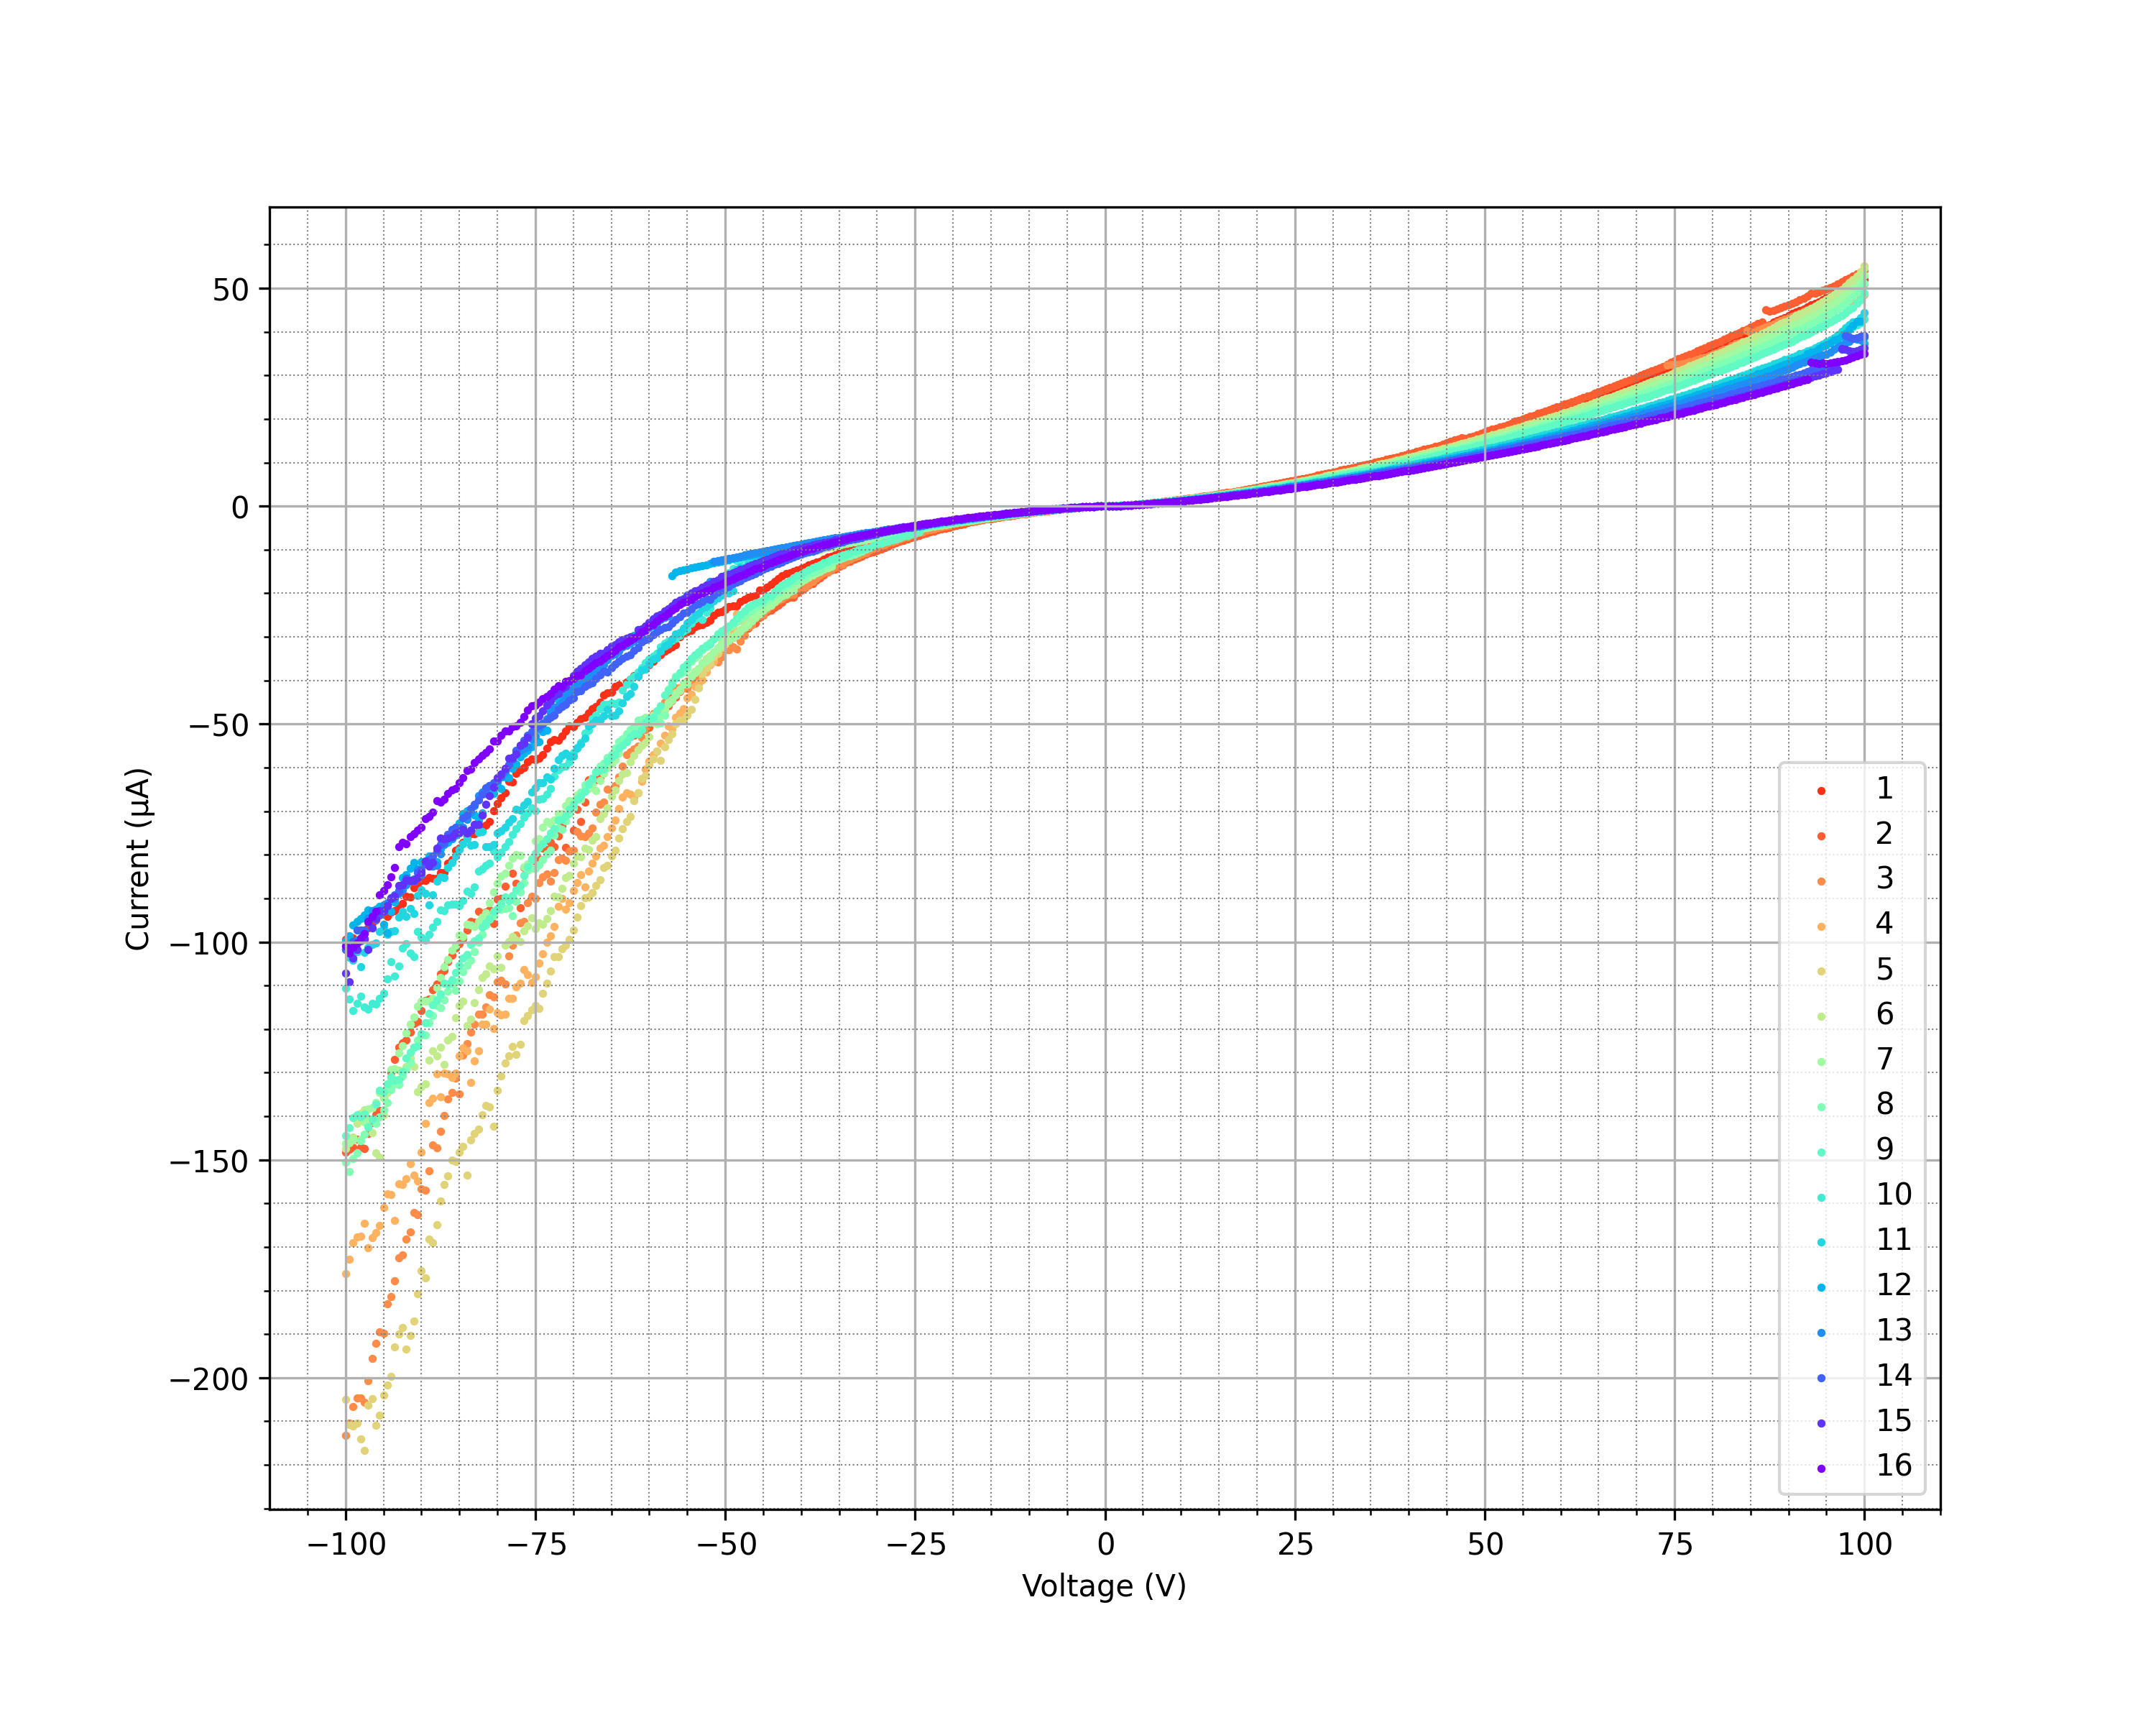
\includegraphics[width=\linewidth]{Chapter7/Figs/Raster/Emitters/124-145_iv.png}
    \caption{The IV characteristics across emitter CH in which significant asymmetry was measured for $\pm$100~\si{\volt}.}
    \label{fig:e_ch_124-145_iv}
\end{figure}

Figure \ref{fig:e_ch_124-145_iv} shows the follow up $\pm100$~\si{\volt} measurements to the asymmetric current observed while running dual-sweep measurements of slightly higher bias. In the positive potential bias region, the Schottky curve is visible. However, in negative bias, a significant, changing asymmetric current was measured. The data are labelled with incrementing numbers, and the legend represents a color map corresponding to the relative dataset indices. At first, the magnitude of current with negative applied voltage increased. After the data indicated by index 5, the current magnitude proceeded to decrease. This trend is also visible in the forward bias region, though the first few sets of data are closely overlapping.

Additionally, after IV sweep 3, characterisation was done with a reverse bias sweep, i.e. the potential bias began at +100~\si{\volt} and swept down to -100~\si{\volt}. This was done to verify that the observed current in the negative bias was not due to the initial starting bias. After IV sweep 5, the probe at position b was re-positioned, taking it off the contact and then placed back. This had no noticeable effect on the IV sweeps. After sweep 9, the probe on location a was similarly re-positioned, with no noticeable change. The final three sets of data were taken with a positive bias sweep, again to verify that the observed characteristics did not change with this change in sweep direction. For clarity, the potential bias was applied to the anode (contact H), and the emitter structure (contact C) was grounded. A strong current at negative bias hence implies that electrons are flowing counter to the intended direction of travel with geometrically enhanced emitter structures.

\begin{figure}[H]
    \centering
    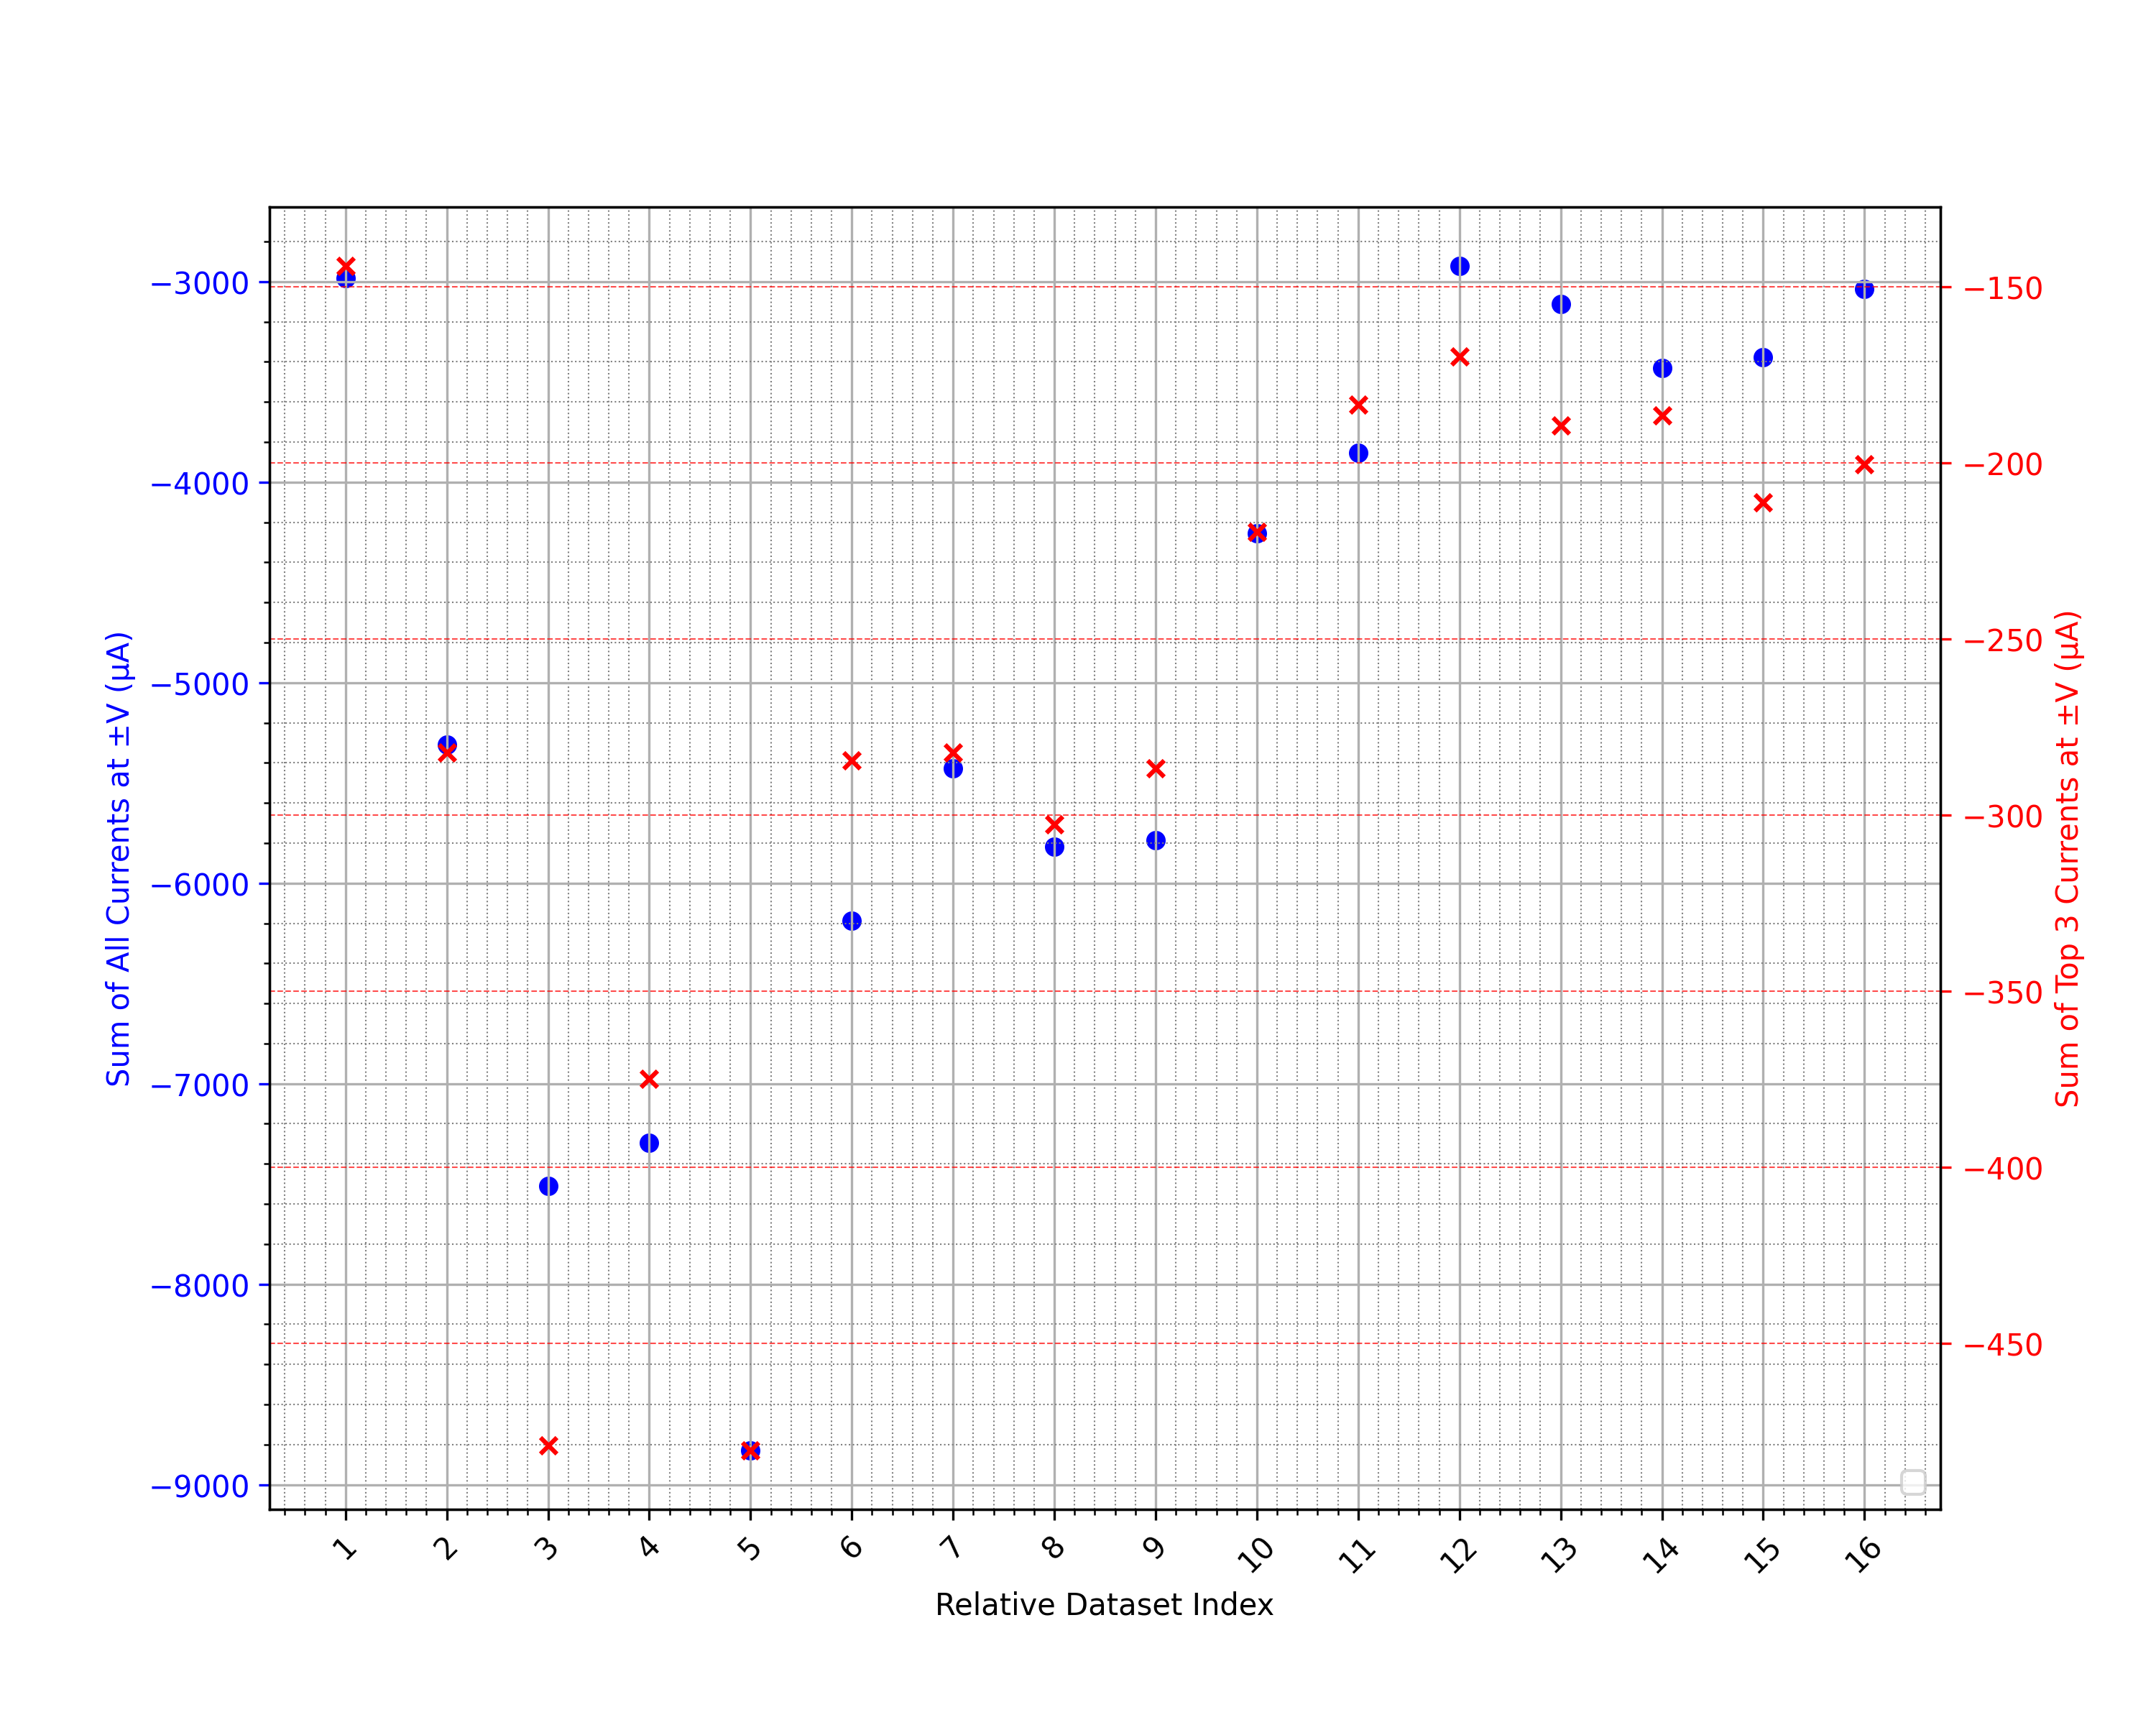
\includegraphics[width=\linewidth]{Chapter7/Figs/Raster/Emitters/124-145_asymmetry.png}
    \caption{The observed asymmetry across emitter CH for $\pm100$~\si{\volt} single sweeps. Blue circles are used for the left y axis, and red crosses are used for the right y axis.}
    \label{fig:e_ch_124-145_asymmetry}
\end{figure}

In contrast to figure \ref{fig:e_ch_5-120v_asymmetry}, which had relatively small levels of asymmetry across the full range of data that may be accounted for by a small percentage error estimation, figure \ref{fig:e_ch_124-145_asymmetry} further underscores the magnitude of asymmetrical current that was observed. The sum of total positive/negative currents are consistently and significantly negative, with the sum of 3 peak positive/negative currents following the same trend. Following these measurements and the observation of changing current over multiple IV sweeps, higher voltage testing was examined to further pursue the asymmetric behaviour observed.

\begin{figure}[H]
    \centering
    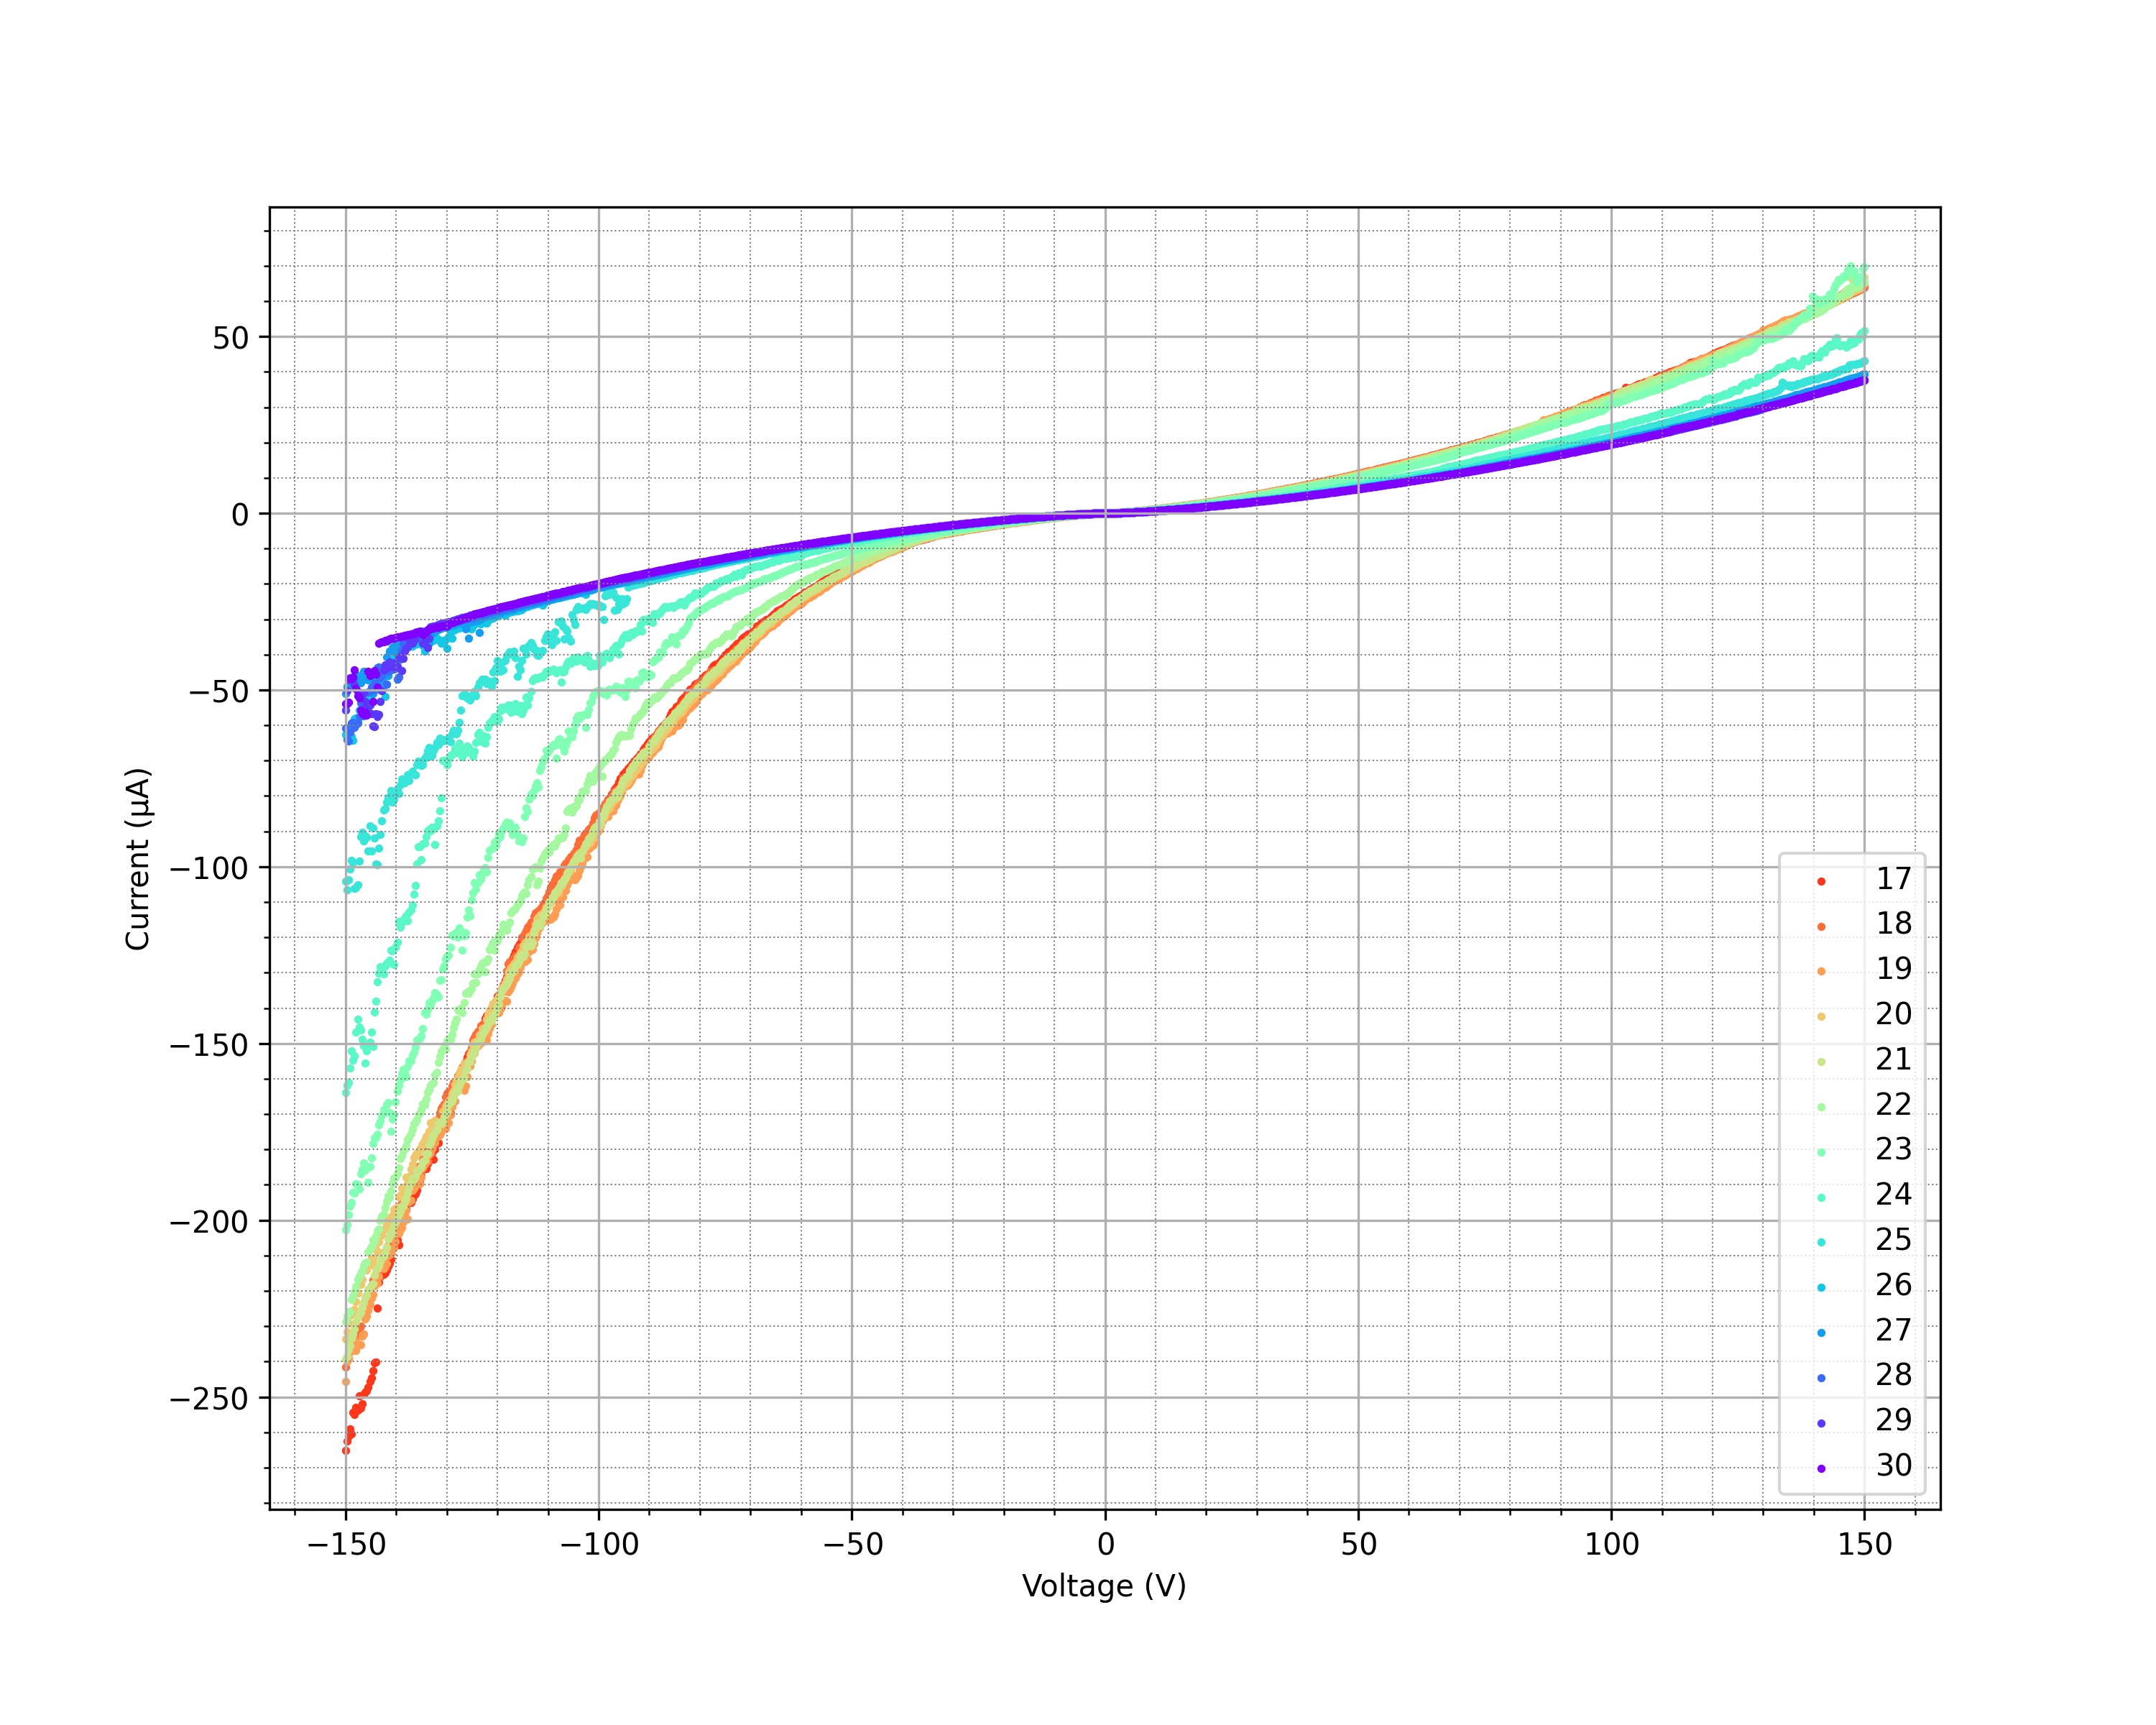
\includegraphics[width=\linewidth]{Chapter7/Figs/Raster/Emitters/146-159_iv.png}
    \caption{The IV characteristics across emitter CH in which significant asymmetry was measured for $\pm$150~\si{\volt}.}
    \label{fig:e_ch_146-159_iv}
\end{figure}

Figure \ref{fig:e_ch_146-159_iv} shows the changing IV characteristics of emitter channel CH with single potential bias sweeps of $\pm$150~\si{\volt}. The 100~\si{\volt} current matches up with relative sweeps 15 and 16 of the previous set of data. Hence, this continues the same decrease in asymmetry as previously observed, but with greater potential bias producing a more significant spread of current in the negative bias region. For this dataset, the number of data points was raised from 401 to 1001, giving a step size of 0.3~\si{\volt}. The IV sweep direction was negative to positive.

\begin{figure}[H]
    \centering
    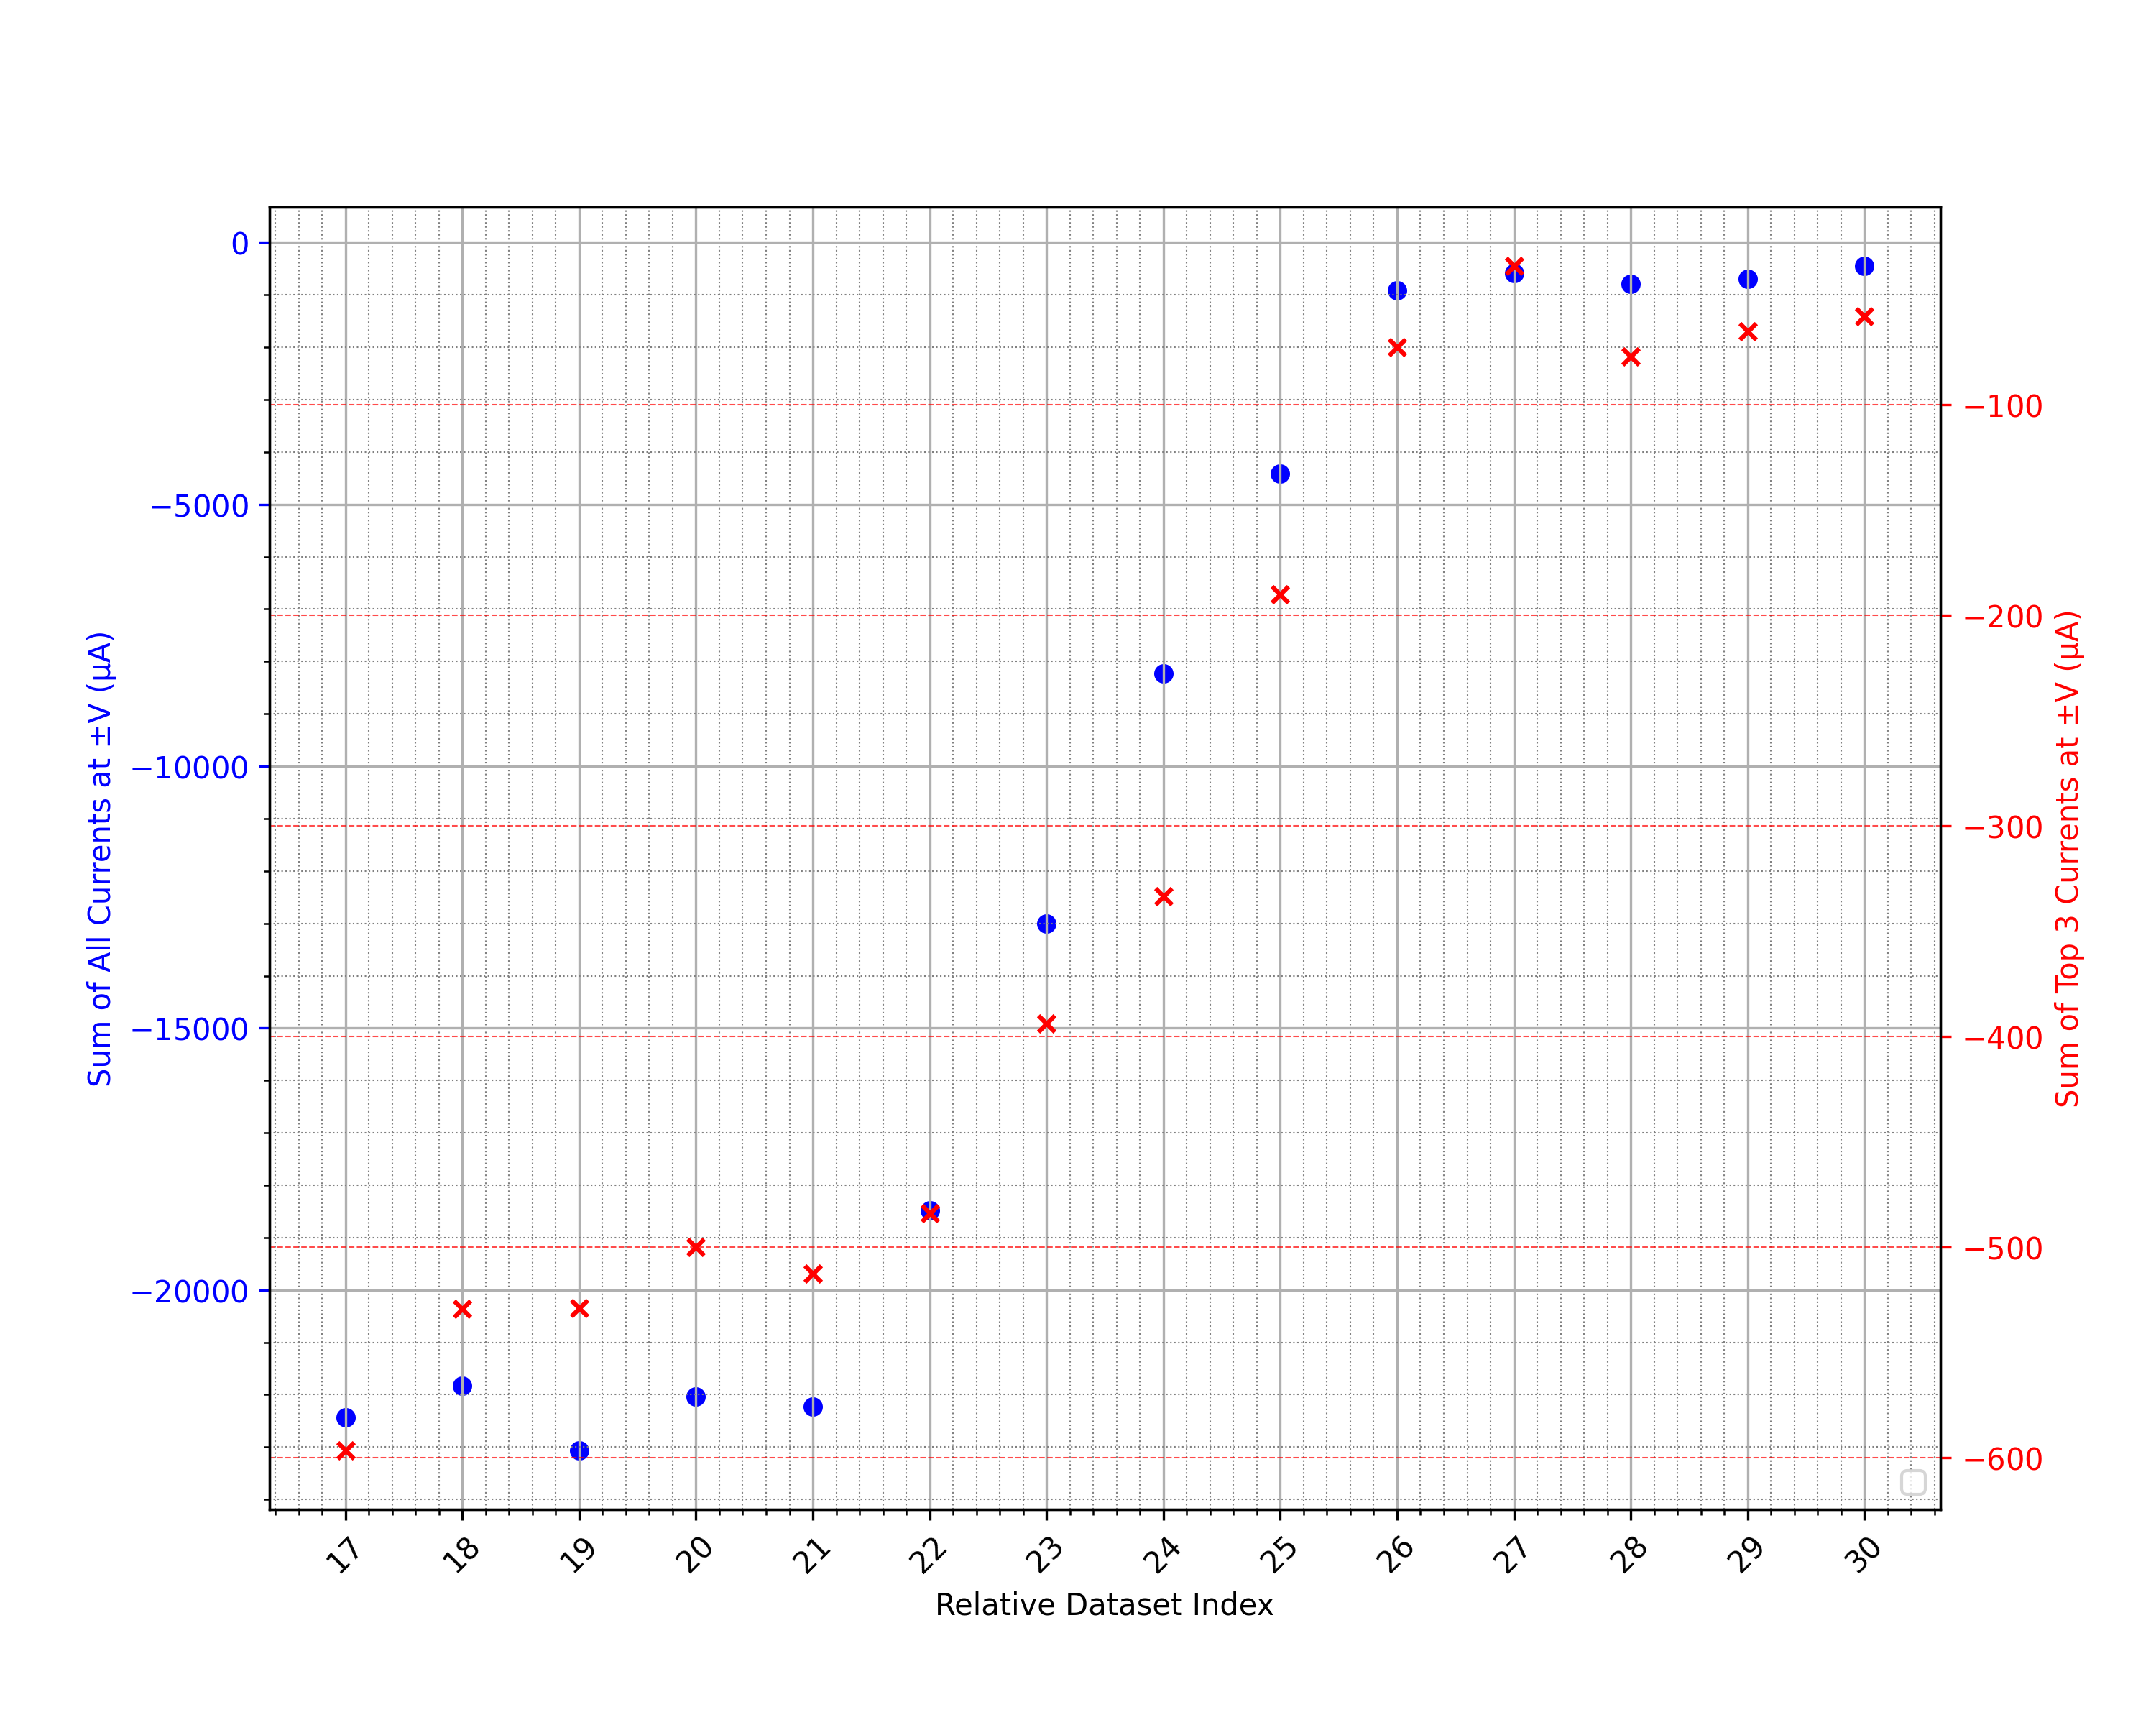
\includegraphics[width=\linewidth]{Chapter7/Figs/Raster/Emitters/146-159_asymmetry.png}
    \caption{The observed asymmetry across emitter CH for $\pm150$~\si{\volt} single sweeps. Blue circles are used for the left y axis, and red crosses are used for the right y axis.}
    \label{fig:e_ch_146-159_asymmetry}
\end{figure}

In figure \ref{fig:e_ch_146-159_asymmetry}, the previously used method of quantifying asymmetry was used to evaluate the $\pm150$~\si{\volt} IV data. As might be expected from the previous sweeps in figure \ref{fig:e_ch_124-145_iv}, the first 4 IV sweeps show a consistent, negative asymmetry, in both the sum of all currents (left axis) and the sum of peak 3 currents (right axis). In contrast to figure \ref{fig:e_ch_124-145_asymmetry}, the final 5 datasets plateau much closer to the 0 mark, indicating that the IV sweeps have returned to near-symmetry.

\begin{figure}[H]
    \centering
    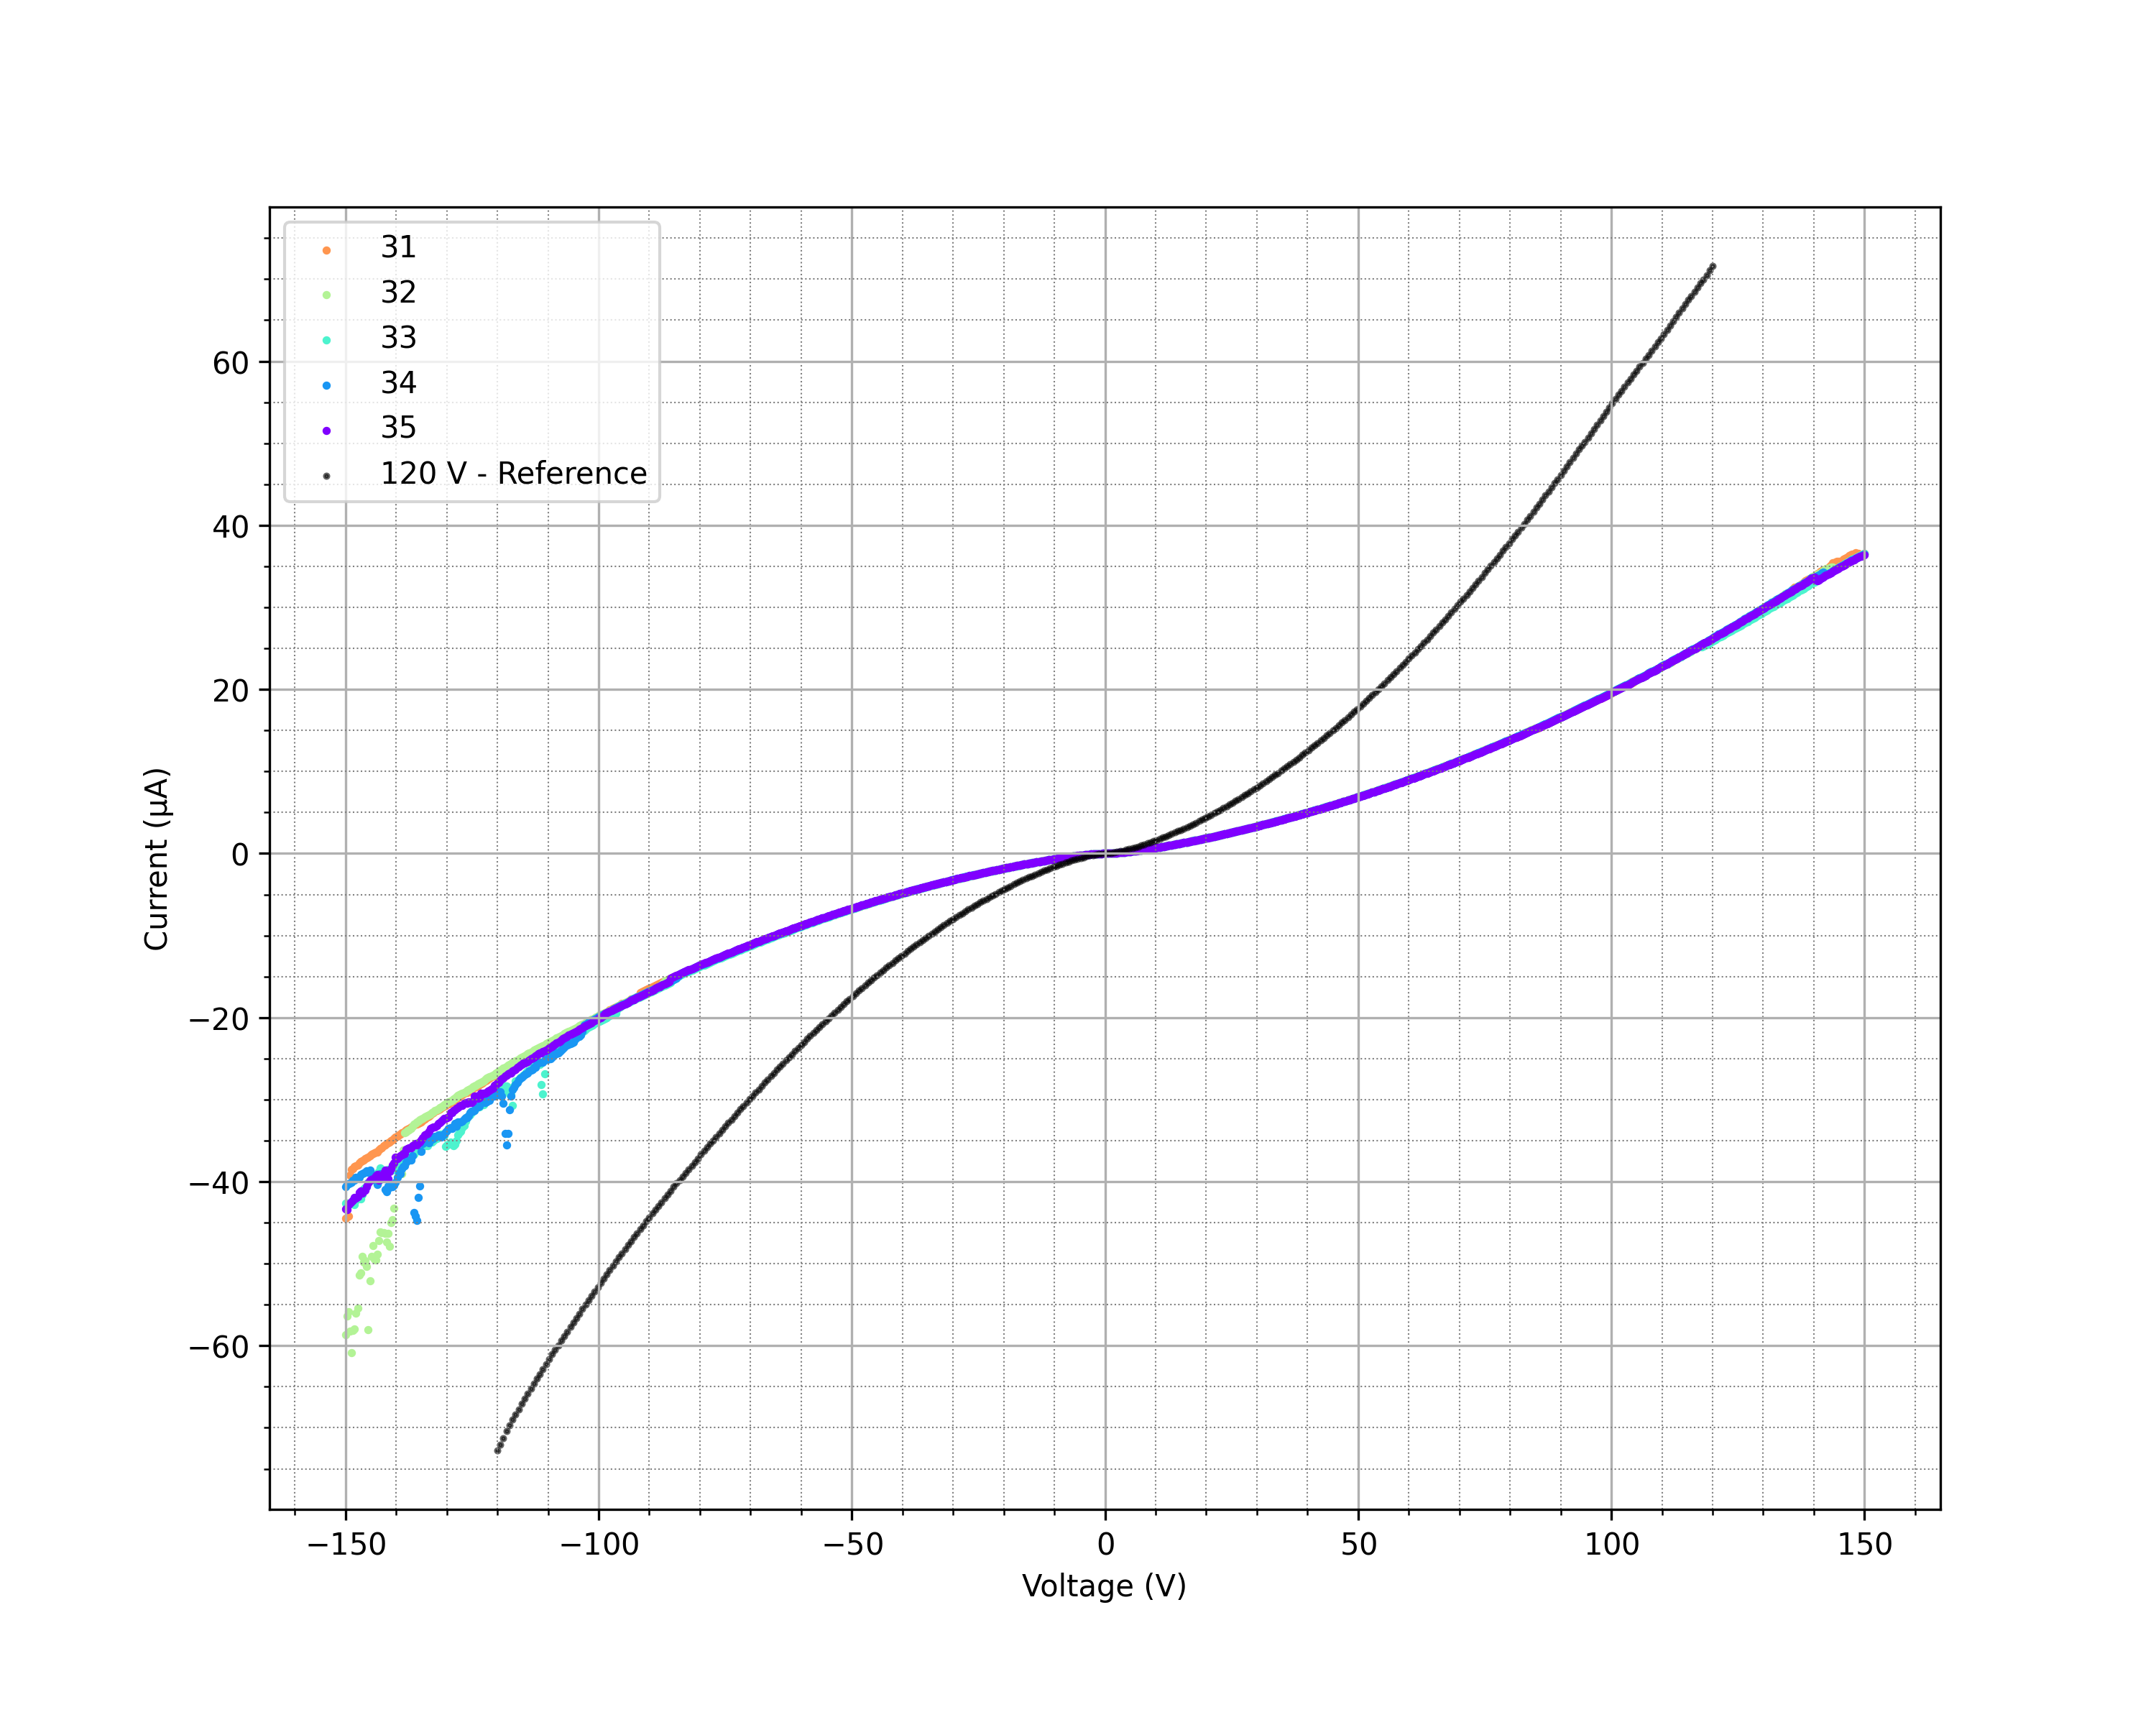
\includegraphics[width=\linewidth]{Chapter7/Figs/Raster/Emitters/160-164_iv.png}
    \caption{The IV characteristics across emitter CH after significant asymmetry was observed, for $\pm$150~\si{\volt} (flipped IV sweep direction).}
    \label{fig:e_ch_160-164_iv}
\end{figure}

Figure \ref{fig:e_ch_160-164_iv} presents the continuation of previous IV sweeps, with another reversal of IV sweep direction. These data are taken with a bias direction of positive to negative, and continues to display the same symmetry as seen in the final few sweeps of figure \ref{fig:e_ch_146-159_iv}. For reference, the first 120~\si{\volt} sweep of this emitter structure is also plotted, to show the disparity between these measurements. It is clear that a change in the electrical properties of this device has occurred. While there is still some noticeable spread in the measured current at peak negative voltages, the data are now generally in agreement for repeated IV sweeps.

\begin{figure}[H]
    \centering
    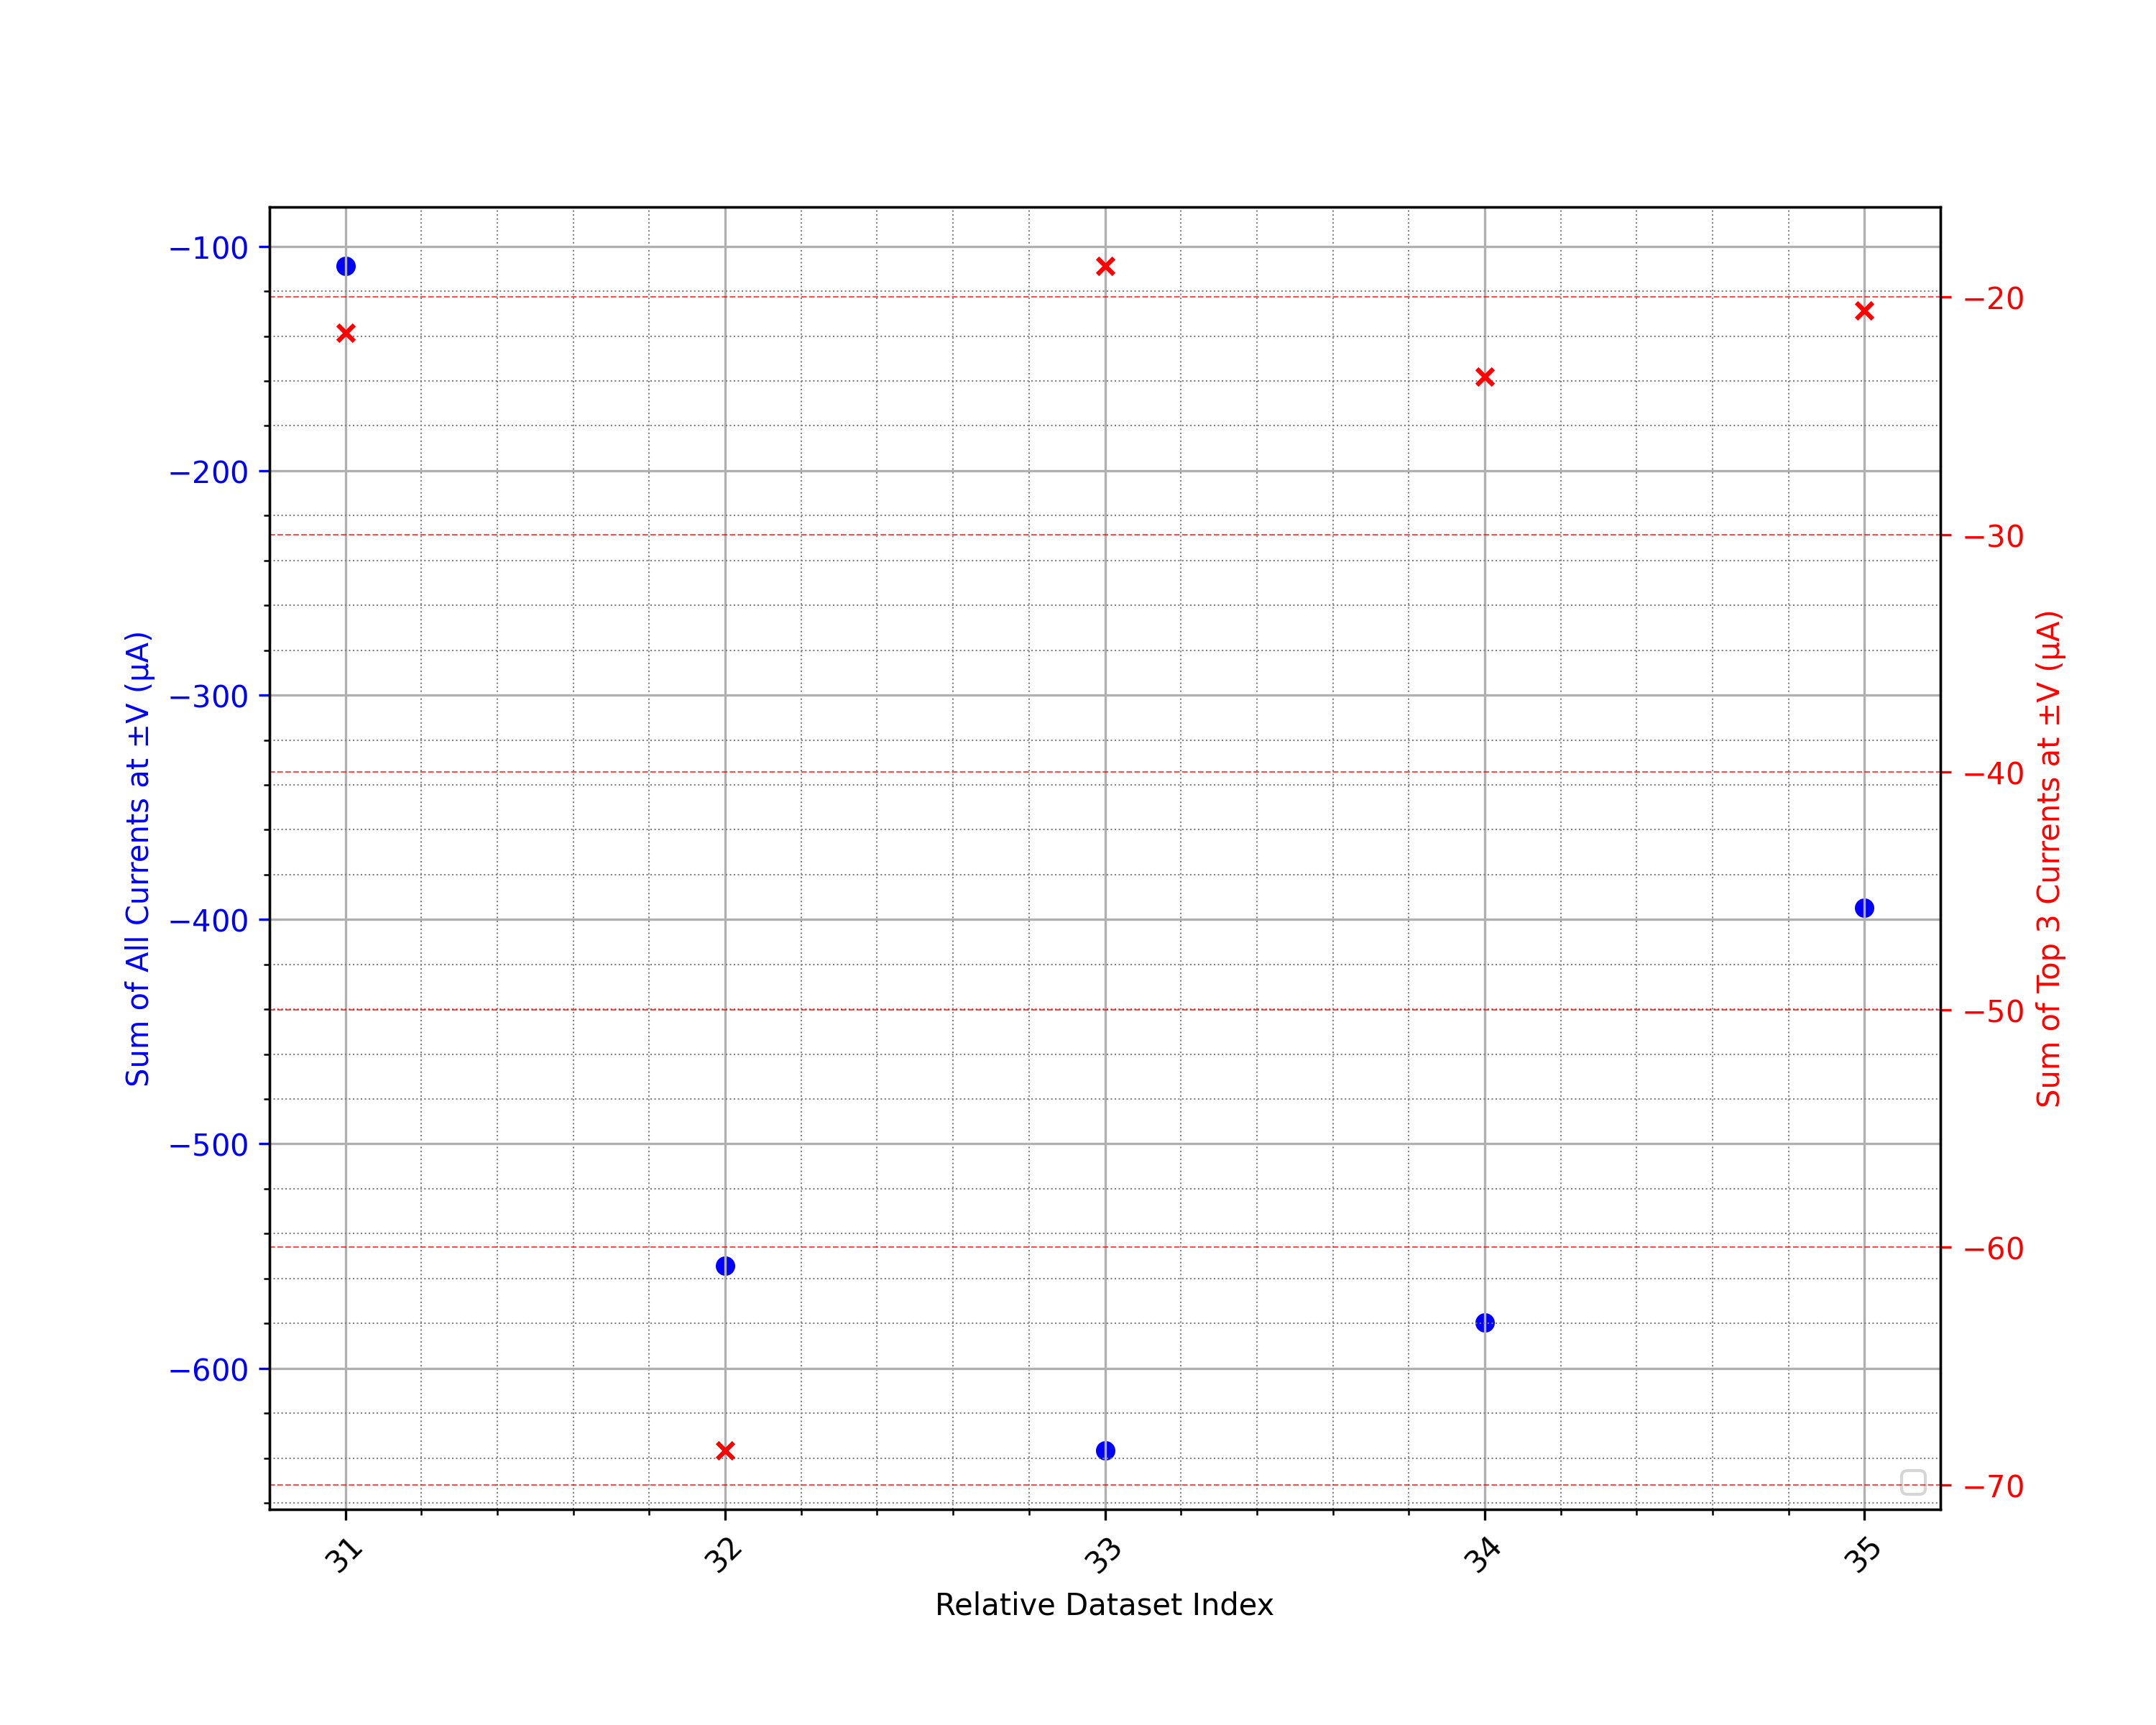
\includegraphics[width=\linewidth]{Chapter7/Figs/Raster/Emitters/160-164_asymmetry.png}
    \caption{The observed asymmetry across emitter CH for $\pm150$~\si{\volt} single sweeps. Blue circles are used for the left y axis, and red crosses are used for the right y axis.}
    \label{fig:e_ch_160-164_asymmetry}
\end{figure}

In figure \ref{fig:e_ch_160-164_asymmetry}, these late stage IV sweeps are examined with the same asymmetry plot as previously used. Compared to the sweeps for which significant asymmetry was present, as for figures \ref{fig:e_ch_124-145_asymmetry, fig:e_ch_146-159_asymmetry}, the channel now appears to be relatively consistent between positive and negative biases, at a sum much closer to 0 for both the sum of total currents and the sum of peak 3 currents. As this now resembles noise, it is reasonable to conclude that the effect causing significant asymmetry has ceased.

\begin{figure}[H]
    \centering
    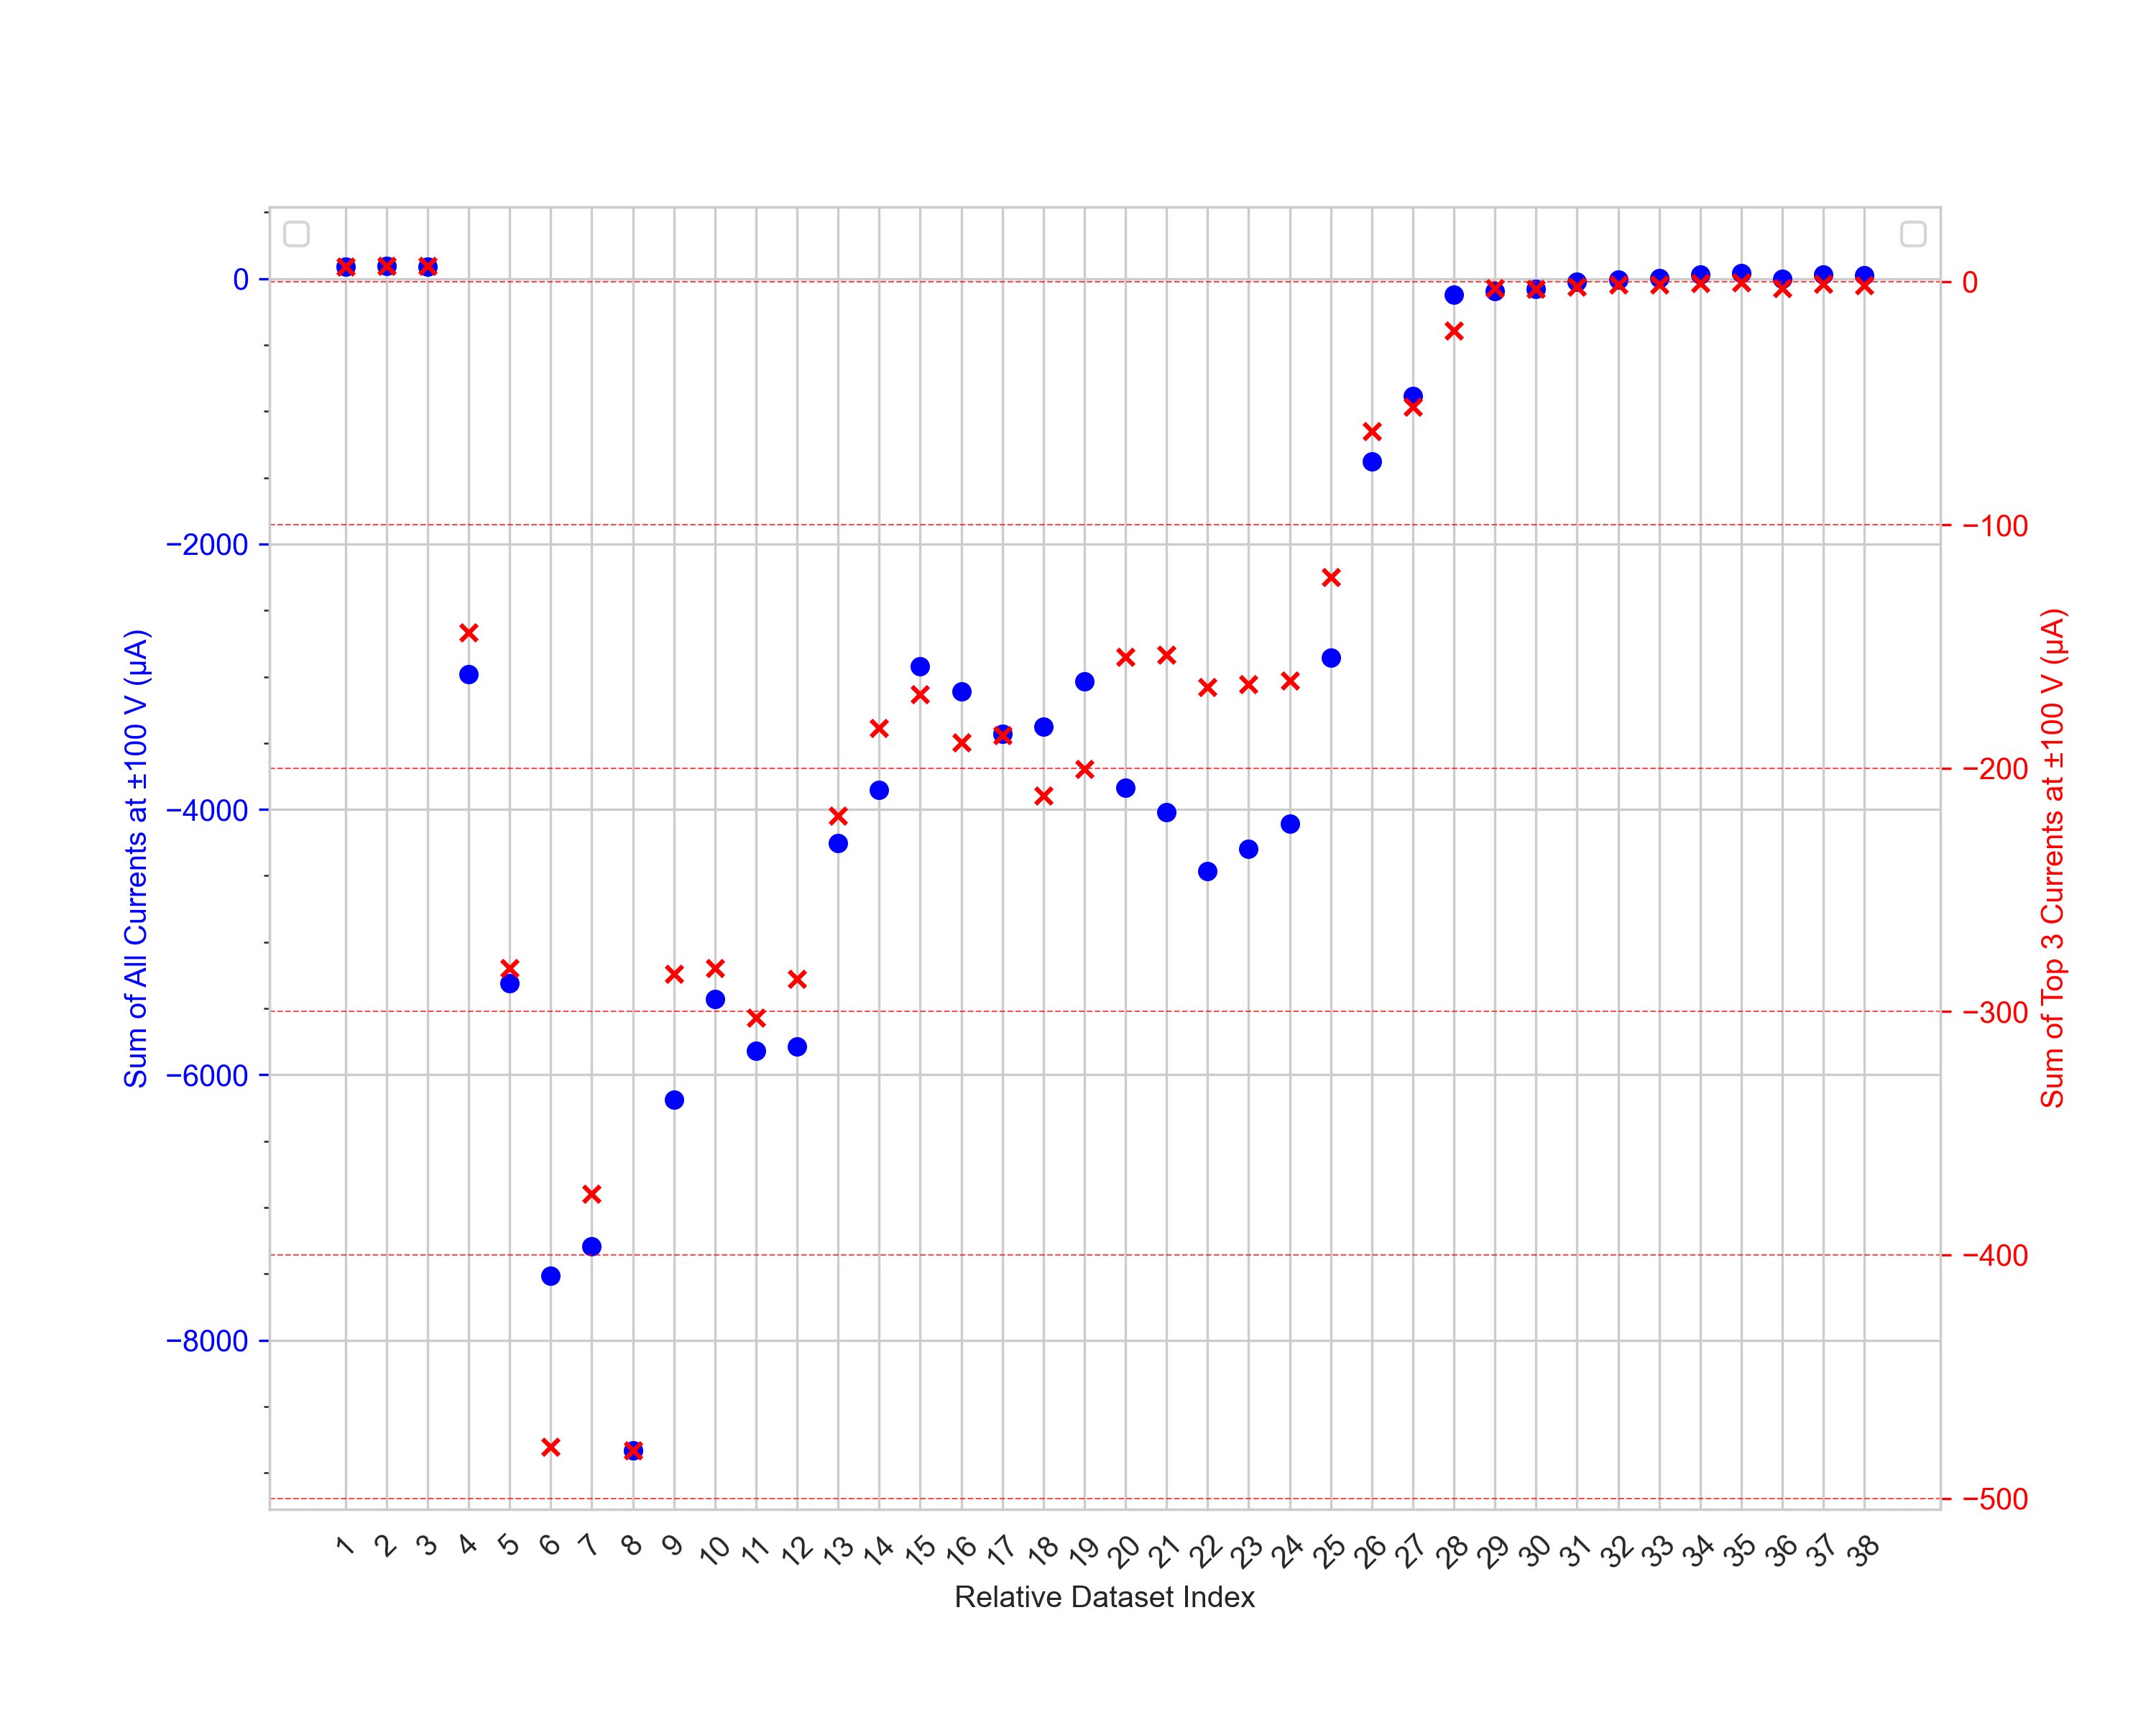
\includegraphics[width=\linewidth]{Chapter7/Figs/Raster/all_asymmetry.png}
    \caption{The observed asymmetry across emitter CH for all single sweeps at $\pm100$~\si{\volt}. Blue circles are used for the left y axis, and red crosses are used for the right y axis.}
    \label{fig:e_ch_all_asymmetry}
\end{figure}

Figure \ref{fig:e_ch_all_asymmetry} provides a full review of the asymmetry profile presented by emitter CH during testing. In this figure, data for $\pm150$~\si{\volt} sweeps are limited to $\pm100$~\si{\volt} to provide direct comparison between these sweeps which were run at differing potential biases. The data included spans the full range of observed behaviour, from the symmetric Schottky profile of early sweeps, through the highly chaotic asymmetry, then back to a symmetrical behaviour for the final sweeps. Further testing with this device did not observe any change from the final sweeps shown here.

\begin{figure}[H]
    \centering
    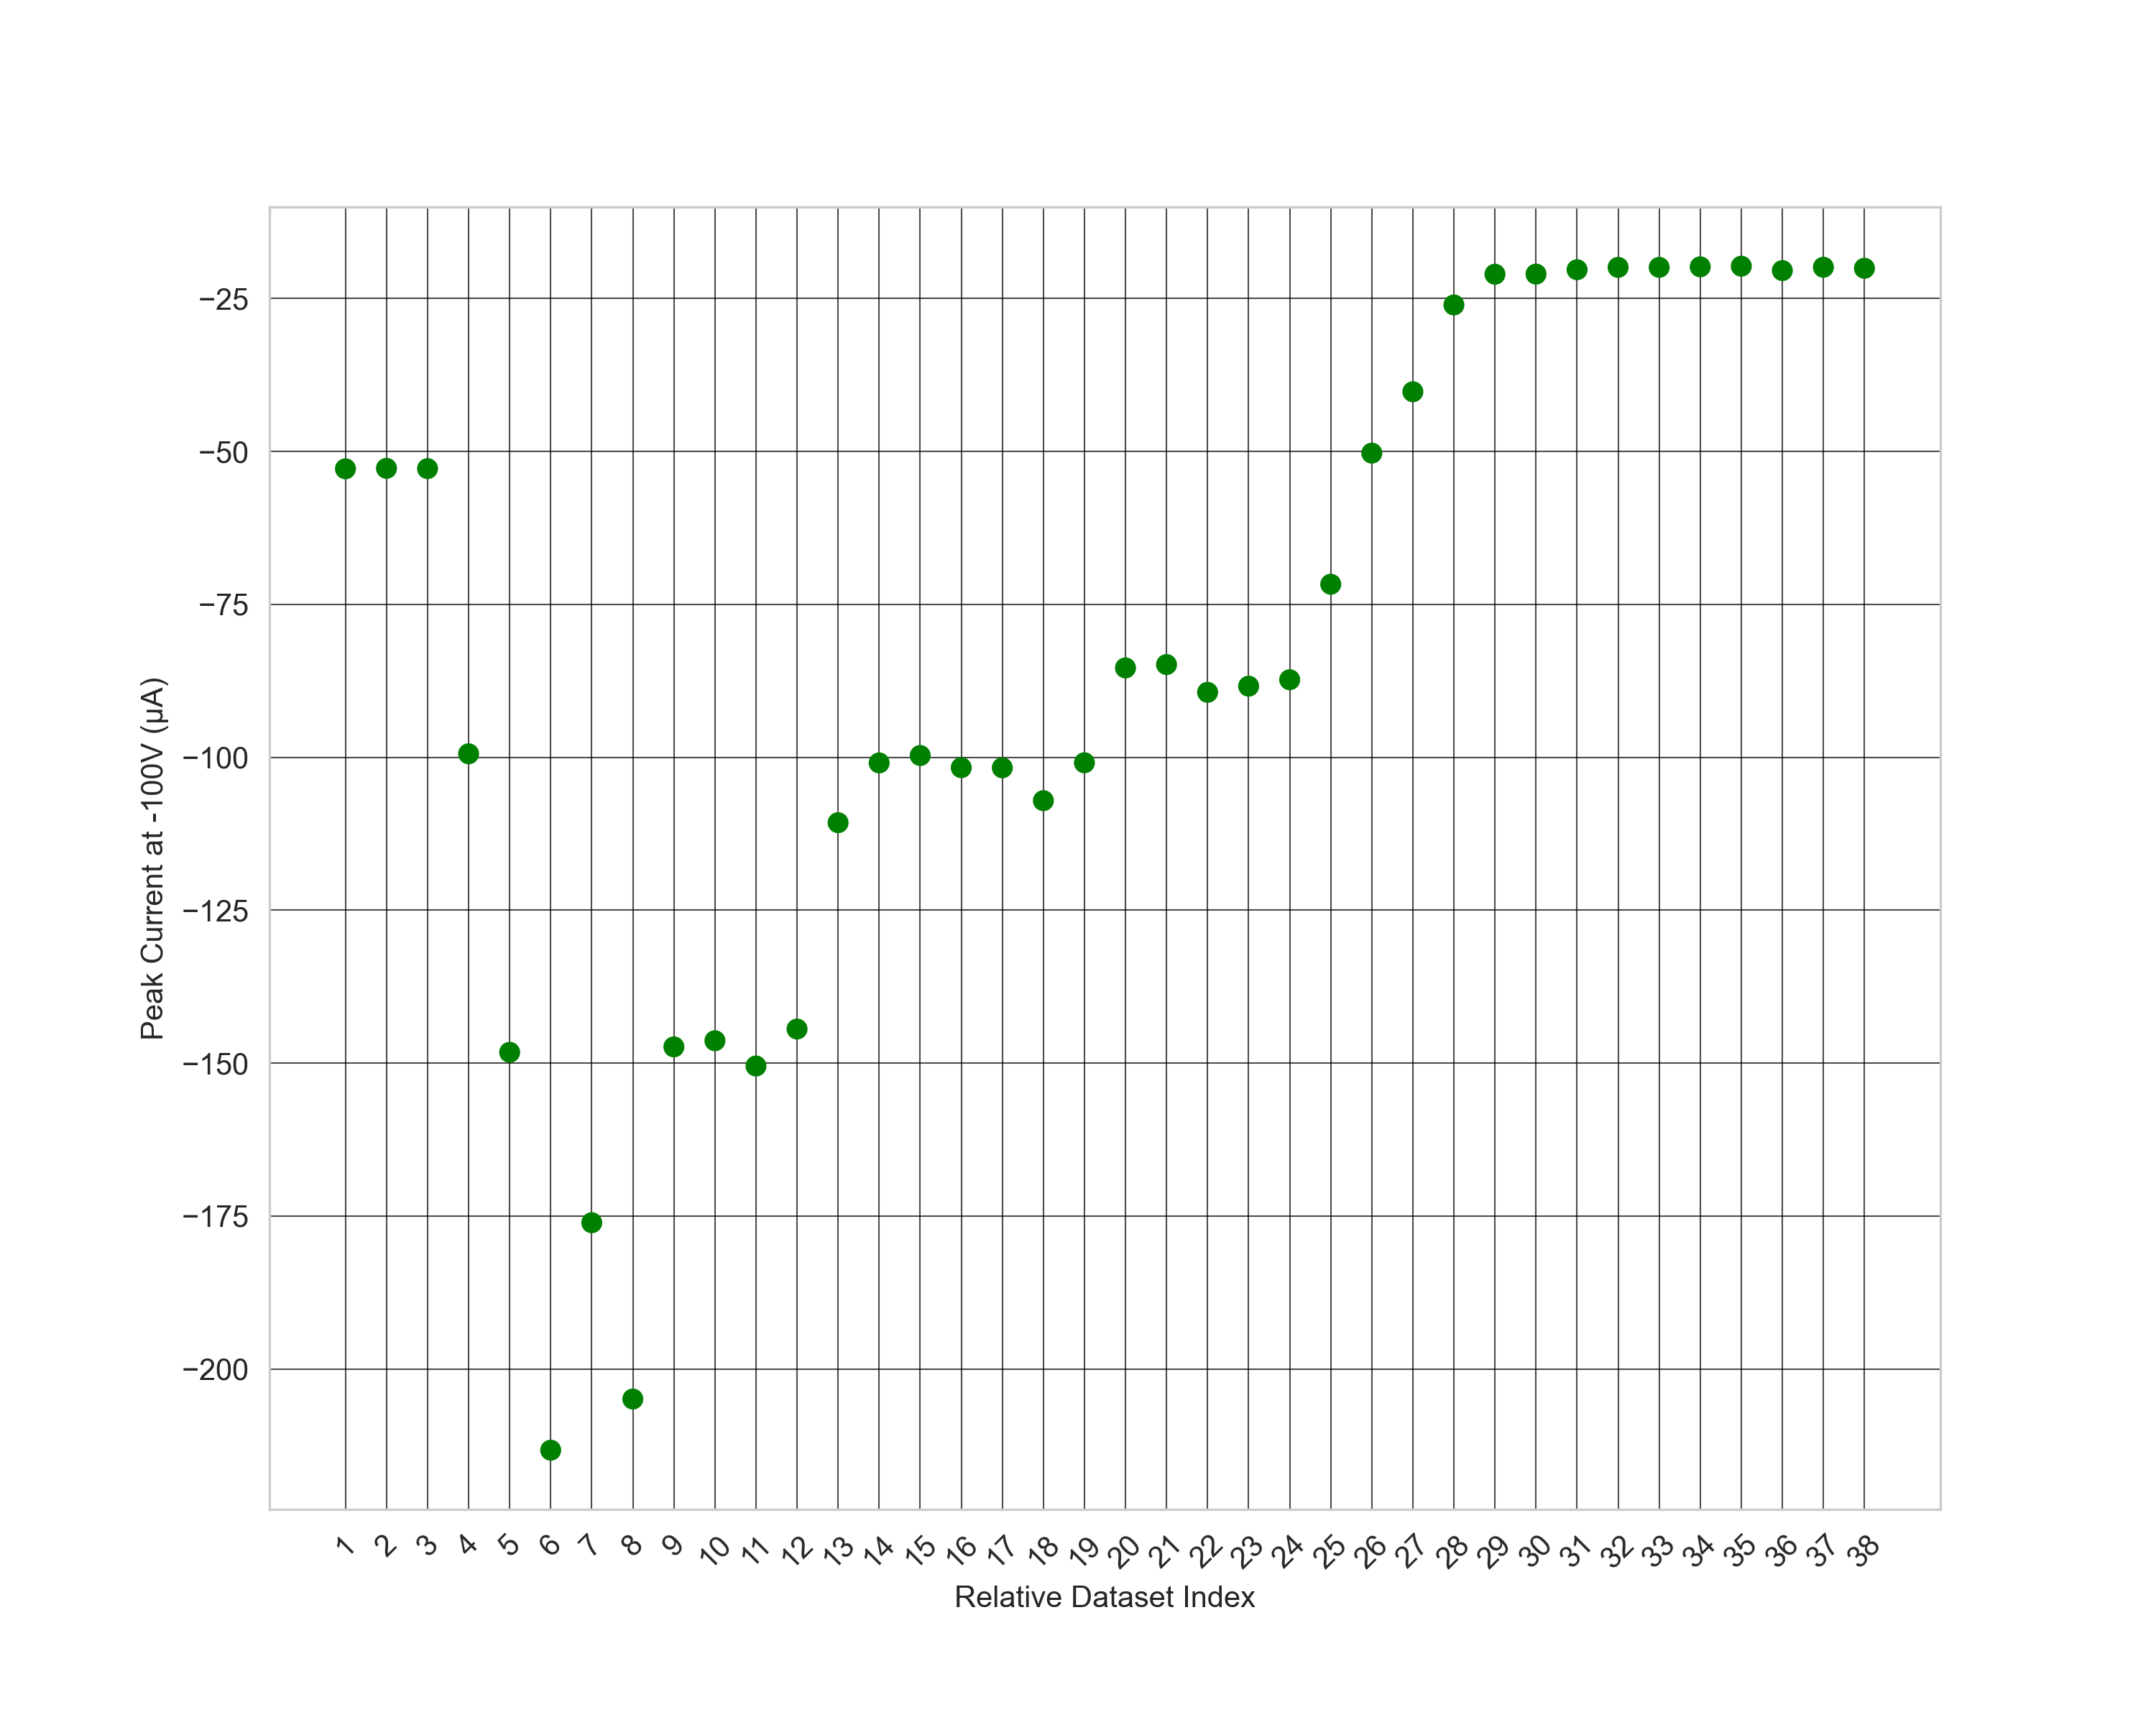
\includegraphics[width=\linewidth]{Chapter7/Figs/Raster/all_peak_current.png}
    \caption{The observed peak currents at -100~\si{\volt}, across all single sweeps.}
    \label{fig:e_ch_all_current}
\end{figure}

Finally, figure~\ref{fig:e_ch_all_current} plots the peak current measured for \(-100~\si{\volt}\) across all sweeps. The trend seen here correlates well with that of the two differing methodologies of quantifying asymmetry, and also provides a quick reference for the peak current values of the IV sweeps shown in Figures~\ref{fig:e_ch_124-145_iv}, \ref{fig:e_ch_146-159_iv}, and \ref{fig:e_ch_160-164_iv}.

\subsubsection{Post-Electrical Characterisation Optical Microscopy}

\begin{figure}[H]
    \centering
    \begin{subfigure}[b]{0.33\textwidth}
        \centering
        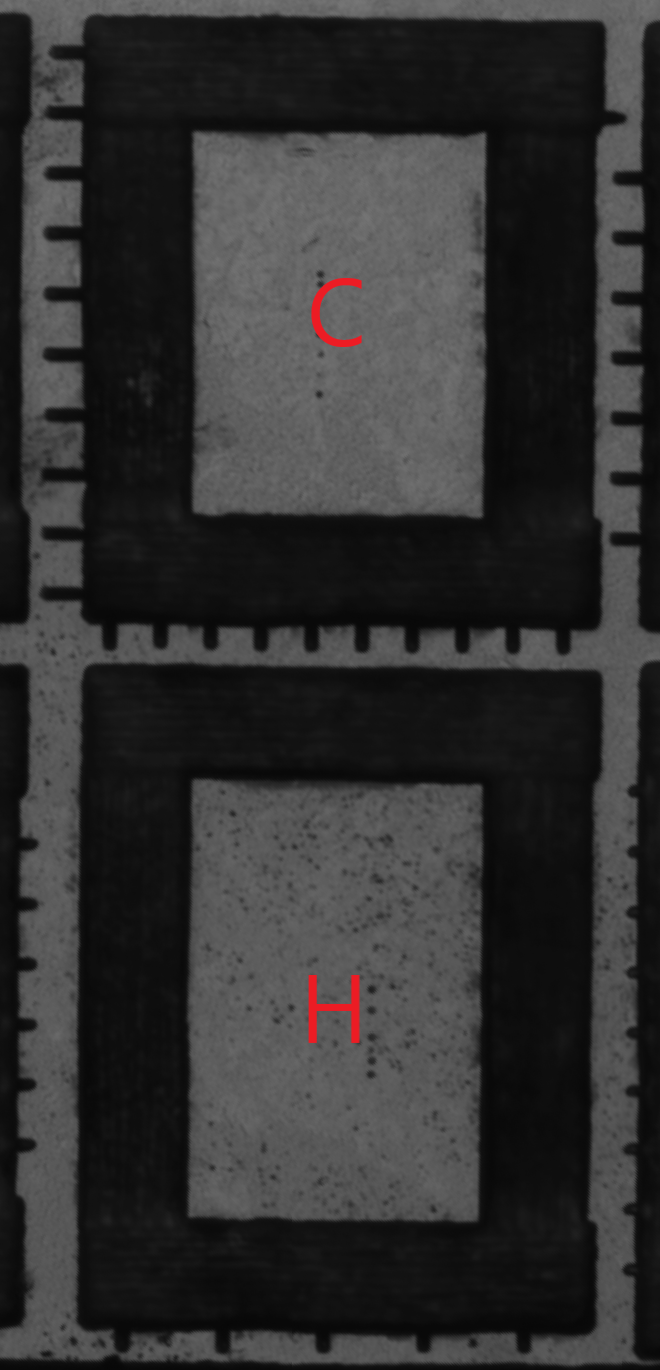
\includegraphics[width=\linewidth]{Chapter7/Figs/Raster/ch_narrow_pre_testing_esid.png}
        \caption{Pre-emitter testing, as seen via 488~\si{\nano\metre} confocal microscopy.}
        \label{fig:ch_narrow_esid}
    \end{subfigure}
    \hfill % spacing between the subfigures
    \begin{subfigure}[b]{0.315\textwidth}
        \centering
        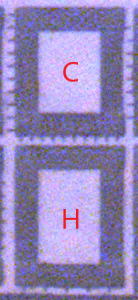
\includegraphics[width=\linewidth]{Chapter7/Figs/Raster/ch_narrow_pre_testing_afm.png}
        \caption{Pre-emitter testing, as seen via back-lit optical microscopy.}
        \label{fig:ch_narrow_afm}
    \end{subfigure}
    \hfill % spacing between the subfigures
    \begin{subfigure}[b]{0.325\textwidth}
        \centering
        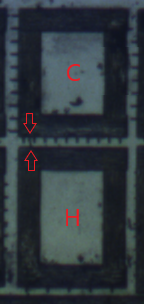
\includegraphics[width=\linewidth]{Chapter7/Figs/Raster/ch_narrow_post_testing_afm1.png}
        \caption{Post-emitter testing, as seen via back-lit optical microscopy.}
        \label{fig:ch_narrow_post_afm}
    \end{subfigure}
    \caption{Optical microscopy of emitter structure CH before and after electrical characterisation.}
    \label{fig:ch_narrow_all}
\end{figure}

Figure \ref{fig:ch_narrow_all} provides three different optical microscopy images of emitter contacts C-H. In \ref{fig:ch_narrow_esid}, the high resolution pre-emitter testing microscopy is given. Figure \ref{fig:ch_narrow_afm} is an optical microscope image taken hours before the time of emitter testing. This image is of lower resolution, but with back lighting, it is qualitatively comparable to that of the high resolution imaging in terms of laser written material clarity. Finally, \ref{fig:ch_narrow_post_afm} provides imaging via the same optical microscopy setup, albeit with better imaging quality due to a longer exposure time and lower ISO setting compared to \ref{fig:ch_narrow_afm}. This reduced the visible noise substantially, but has similar issues with resolution of minimum feature sizes in comparison to the 488~\si{\nano\metre} confocal microscopy. Regardless, a clear distinguishing feature within the emitter channel is visible, highlighted with a pair of red arrows. Surface contaminants can be seen within the rectangular wire contacts of C and H, on the diamond surface itself, and are visible as small, roundish features. The feature indicated within the channel is similar to the written emitter wires, spanning the full channel width, and is narrow and wire-like. Hence, this may represent a tangible change in the emitter channel itself due to the high voltage testing.

\section{Numerical Modelling}
\label{sec:modelling}
Following the observation of a significant negative current flow asymmetry in the testing of emitter structure CH, further numerical modelling was performed in an attempt to elucidate the possible physical origin of this transient current at high negative biases. A particular concern was the mechanism of current injection into the phosphorous doped diamond channel and the possibility of observing field effect emission due to the sharp emitters.

\subsection{Schottky Junctions}
The back to back Schottky junction is a challenging device to model accurately. Numerical methods in this area often rely upon various approximations and boundary conditions to allow for simulations which provide convergence, with models ranging from earlier works in which the two Schottky barriers are assumed to have the same heights and ideality factors \cite{Nam2005, Ramirez2006, Nagano2007}, to more complete models which allow for variance between the two barriers \cite{Nouchi2014, Wang2020, Grillo2020, DiBartolomeo2018, DiBartolomeo2019, DiBartolomeo20192}. It is worth noting that single Schottky barriers can be challenging in their own right to model accurately, with significant work in the field of numerical modelling focused on single barriers, and the application of these barriers within devices \cite{Furno2007, Wu2022, Splith2021}. This is especially true for wide bandgap semiconductors in which significant Fermi level pinning is observed, such as SiC \cite{Baum2022}, as well as diamond \cite{Wang2022, Han2023}. For the purposes of examining predicted current flow due to thermionic and field effect emission, and identifying the dominant mechanism, simplified models of the emitter were used to attempt to resolve the origin of the observed asymmetry within the CH emitter structure.

\subsection{Ideal Schottky Equations Used}
The relevant equations which are used to solve for an ideal Schottky contact are given as outlined by Crowell \cite{crowell:1966} and Sze \cite{sze2006}. The semiconductor is assumed to be nondegenerate, with the contact acting as a source or sink for carriers with surface recombination mechanism:
\begin{align}
    \bm{J}_{n} \cdot n &= -q v_{n} (n - n_{0}) \\
    \bm{J}_{p} \cdot n &= q v_{p} (p - p_{0})
\end{align}
\noindent where $\bm{J_{n,p}}$ are the outward normal electron and hole current densities respectively, $n$ is the outward normal electron concentration in the semiconducting region, $v_{n,p}$ are the recombination velocities for electrons and holes and $n_{0}, p_{0}$ are the quasi-equilibrium carrier densities of electrons and holes. These quasi-equilibrium carrier densities are determined via:
\begin{align}
    n_0 = N_{c} \exp \left( -\frac{E_{c} - E_{fm}}{k_{B} T} \right) = N_{c} \exp \left( -\frac{\phi_{B}}{k_{B} T} \right), \\
    p_0 = N_{v} \exp \left( -\frac{E_{fm} - E_{v}}{k_{B} T} \right) = N_{v} \exp \left( -\frac{E_{g} - \phi_B}{k_{B} T} \right)\\
    \phi_{B} = \phi_{m}-\chi
\end{align}
\noindent in which $\phi_{m}$ is the metal work function, $\chi$ is the semiconductor electron affinity, $E_{fm}$ is the metal Fermi level and crucially $\phi_{b}$ is the barrier height for electrons from the metal into the semiconductor. Also given are $E_{c,v}$ which are the conduction and valence band energy levels respectively, $E_{g}$ is the bandgap energy, $N_{c,v}$ are the effective density of states in the conduction and valence band, $T$ is the absolute temperature and $k_{B}$ is the Boltzmann constant. The recombination velocities in the case of dominant thermionic emission are determined as \cite{Shur1990}:
\begin{align}
    v_{n} = \frac{A^{*}_{n} T^2}{q N_{c}} \\
    v_{p} = \frac{A^{*}_{p} T^2}{q N_{v}}
\end{align}
\noindent where $A^{*}_{n,p}$ are the effective Richardson's constants for electrons and holes respectively. Finally, the boundary condition on voltage is determined as:

\begin{equation}
    V = - \left( \phi_{B} + \chi \right) - \frac{\Delta E}{q} + V_{0}
\end{equation}
\noindent where $V_{0}$ is an applied bias and $\Delta E$ is the shift in band edges.

\subsection{Approximate Model}
To computationally simulate emitter structure CH within COMSOL Multiphysics, a few assumptions are taken to simplify the model for comparison of thermionic and field effect emission. First and foremost is the usage of an ohmic anode. This is primarily due to the issues with convergence associated with a diamond double Schottky device, but is a practical way to focus on the current emission as limited by the cathode side of the emitter junction. While this approximation may not accurately model the total current that is measured, it will provide a clear description of current due to the geometrically enhanced Schottky contact.

A second assumption that resulted from attempts to model diamond based electronic devices at large is the usage of a totally ionised donor concentration at $4.2\times10^{14}$~\si{\per\centi\metre\cubed}. Incomplete ionisation models were implemented in trial models, but the slight variability in active donor concentration was negligible, especially given the experimental emitter data taken at room temperature being well within the freeze out area for phosphorous doped diamond. The concentration used hence represents the calculated estimate for active dopant concentration within phosphorous doped diamond at this temperature.

Finally, a Murphy-Good or Good-M\"{u}ller form of field effect emission is used to approximate the injected current density due to geometric enhancement of the local magnitude in electric field norm \cite{Good1956, Kyritsakis2015}:

\begin{equation}
    J_{GM} = \frac{aF_{eff}^{2}}{\phi_{m}}\exp{-\frac{b\phi_{m}^{1.5}}{F_{eff}}}
    \label{eq:good-muller}
\end{equation}

\noindent where $a=1.54\times10^{-6}$~\si{\micro\ampere\electronvolt\per\volt\squared} and $b=6.83$~\si{\electronvolt^{-3/2}\volt\per\nano\metre} are the standard Fowler-Nordheim constants, $F_{eff}$ is the effective local electric field norm, defined as $F_{eff} = \sqrt{E_{x}\cdot E_{x} + E_{y}\cdot E_{y} + E_{z}\cdot E_{z}}$. This may also be referred to as the amplitude of the electric field, and is defined for each element in the finite mesh used in finite element modelling (FEM). This form of field effect emission represents one of the simplest approximations of this class of equations, with more complete derivations providing further precision in an extended Murphy-Good equation \cite{Forbes2019}. However, for the purposes of estimating field effect emission, this highly simplified form of the equation was implemented. Also note that in the following models a metal work function $\phi_{m}=4.5$~\si{\electronvolt} is utilised, which is another assumption that can significantly effect the Schottky thermionic emission.

\subsection{Full Array Electrostatics}
To begin with, it is necessary to consider the larger scale situation of an emitter array, as the non planar geometry may introduce irregularities on the larger scale. In this model, the electrostatics were calculated, with the electric field norm in particular examined as this is the driving factor in all forms of field effect emission.

\begin{figure}[H]
    \centering
    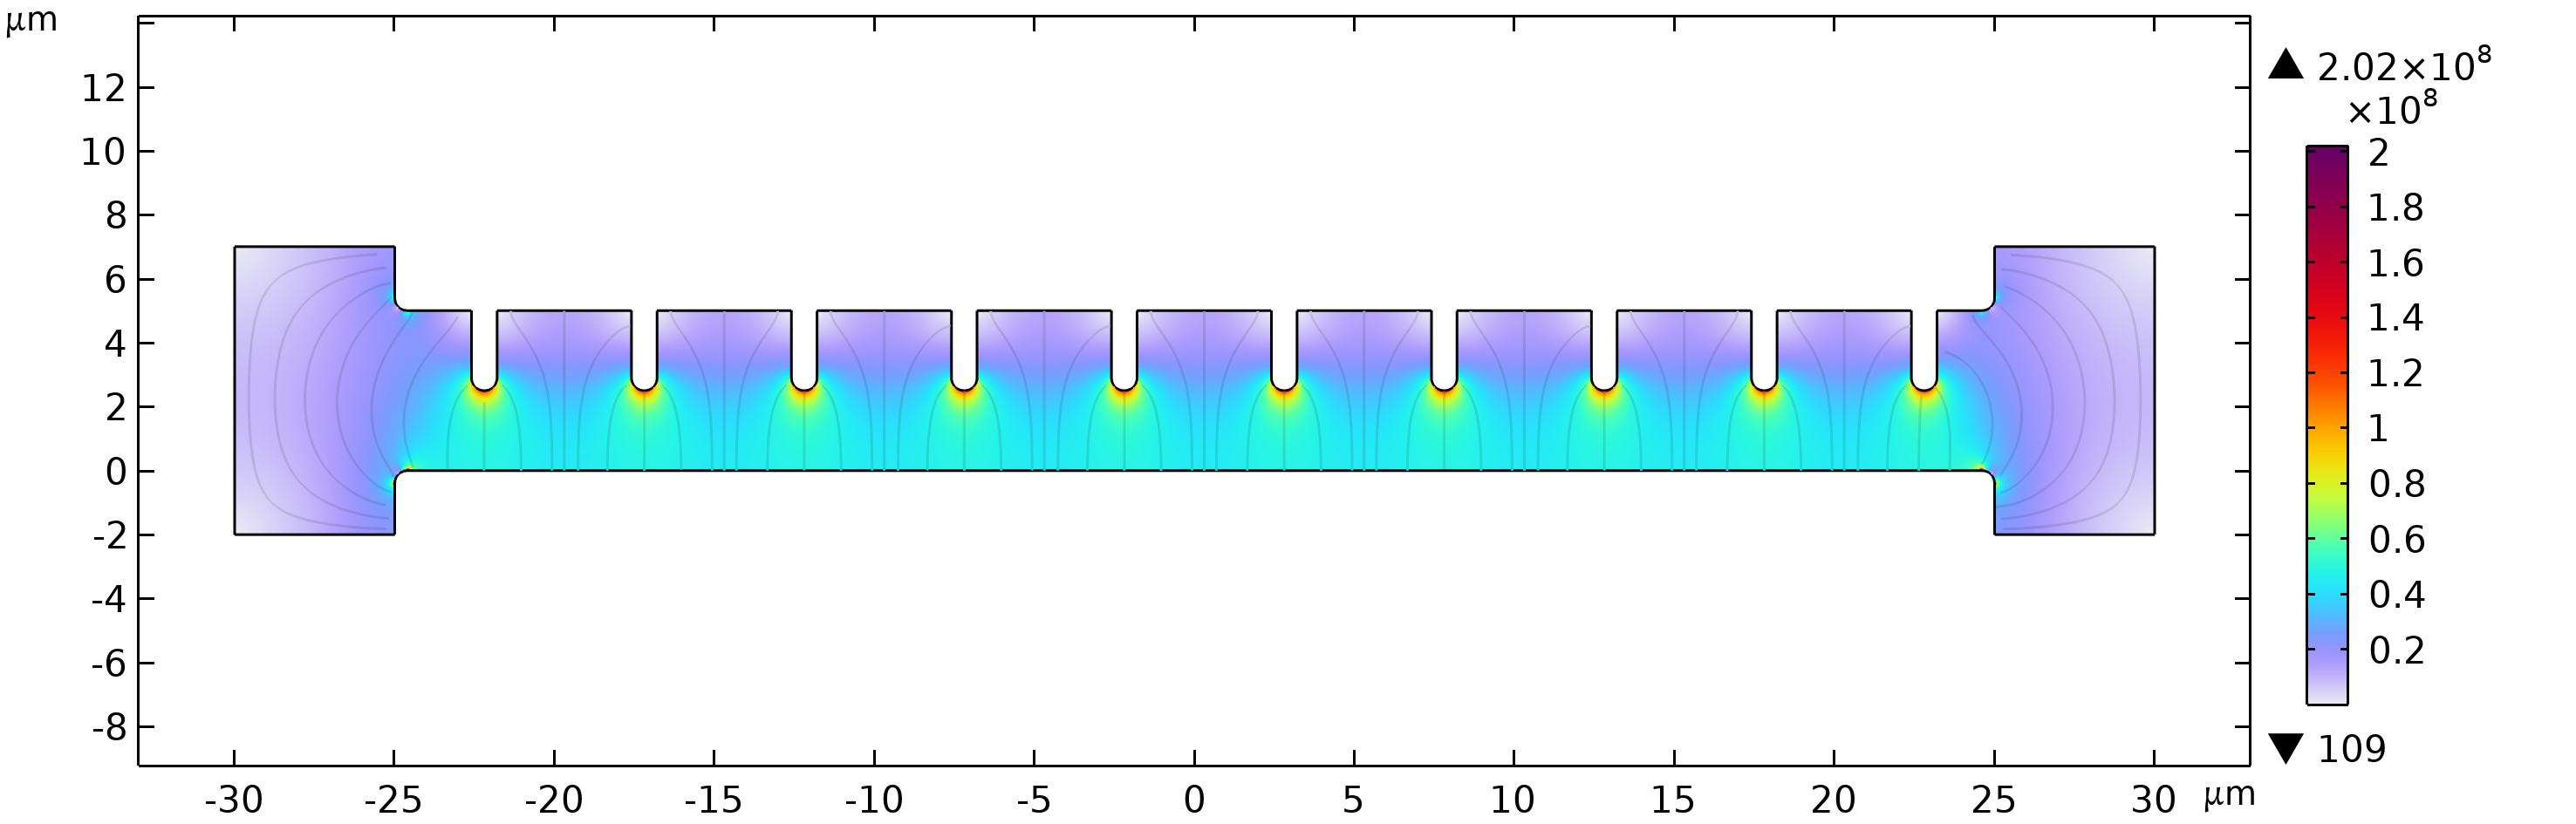
\includegraphics[width=\linewidth]{Chapter7/Figs/Raster/Comsol/+150_array_es.png}
    \caption{The electric field norm of an idealised geometry for emitter array CH.}
    \label{fig:c_150_array_es_norme}
\end{figure}

\begin{figure}[H]
    \centering
    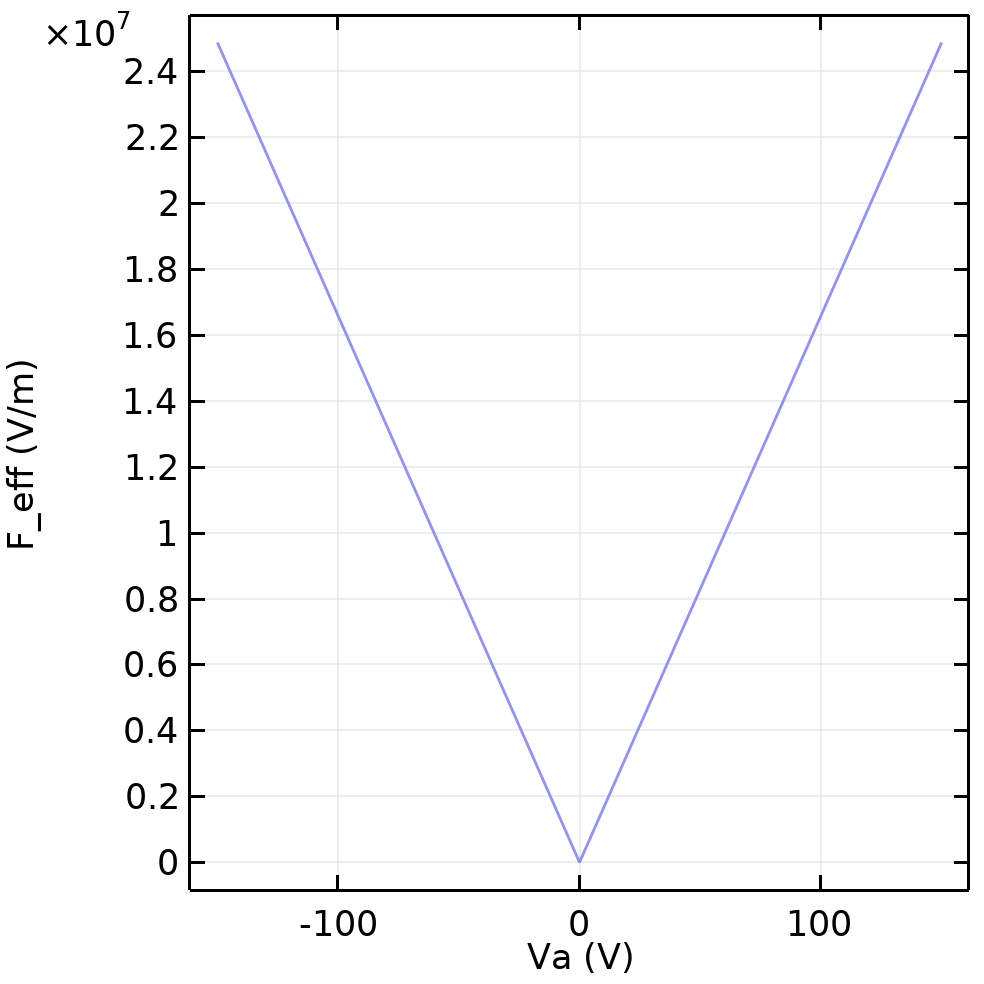
\includegraphics[width=0.5\linewidth]{Chapter7/Figs/Raster/Comsol/array_es_full.png}
    \caption{The peak electric field norm on the cathode structure for $\pm150$~\si{\volt}.}
    \label{fig:c_array_es_full}
\end{figure}

In figures \ref{fig:c_150_array_es_norme} and \ref{fig:c_array_closer}, the idealised geometry and resulting electric field norm surface plot is shown for an anode bias ($V_{a}$) of +150~\si{\volt}. Note that the cathode is held at 0~\si{\volt}. For an earlier discussion of the emitter tip profile as modelled, please see section \ref{subsec:emitter_sharpness}. This electrostatic model was used for the full $\pm150$~\si{\volt} range, with the resulting electric field norm maximum for the cathode plotted in figure \ref{fig:c_array_es_full}. The slight discrepancy between peak electric field norm in this figure when compared to the full geometry of figure \ref{fig:c_150_array_es_norme} can be attributed to meshing. However, the electric field norm of well over $1\times10^{7}$~\si{\volt\per\metre} is substantial, and is consistent across the differing emitters in this ideal geometry setup.

\begin{figure}[H]
    \centering
    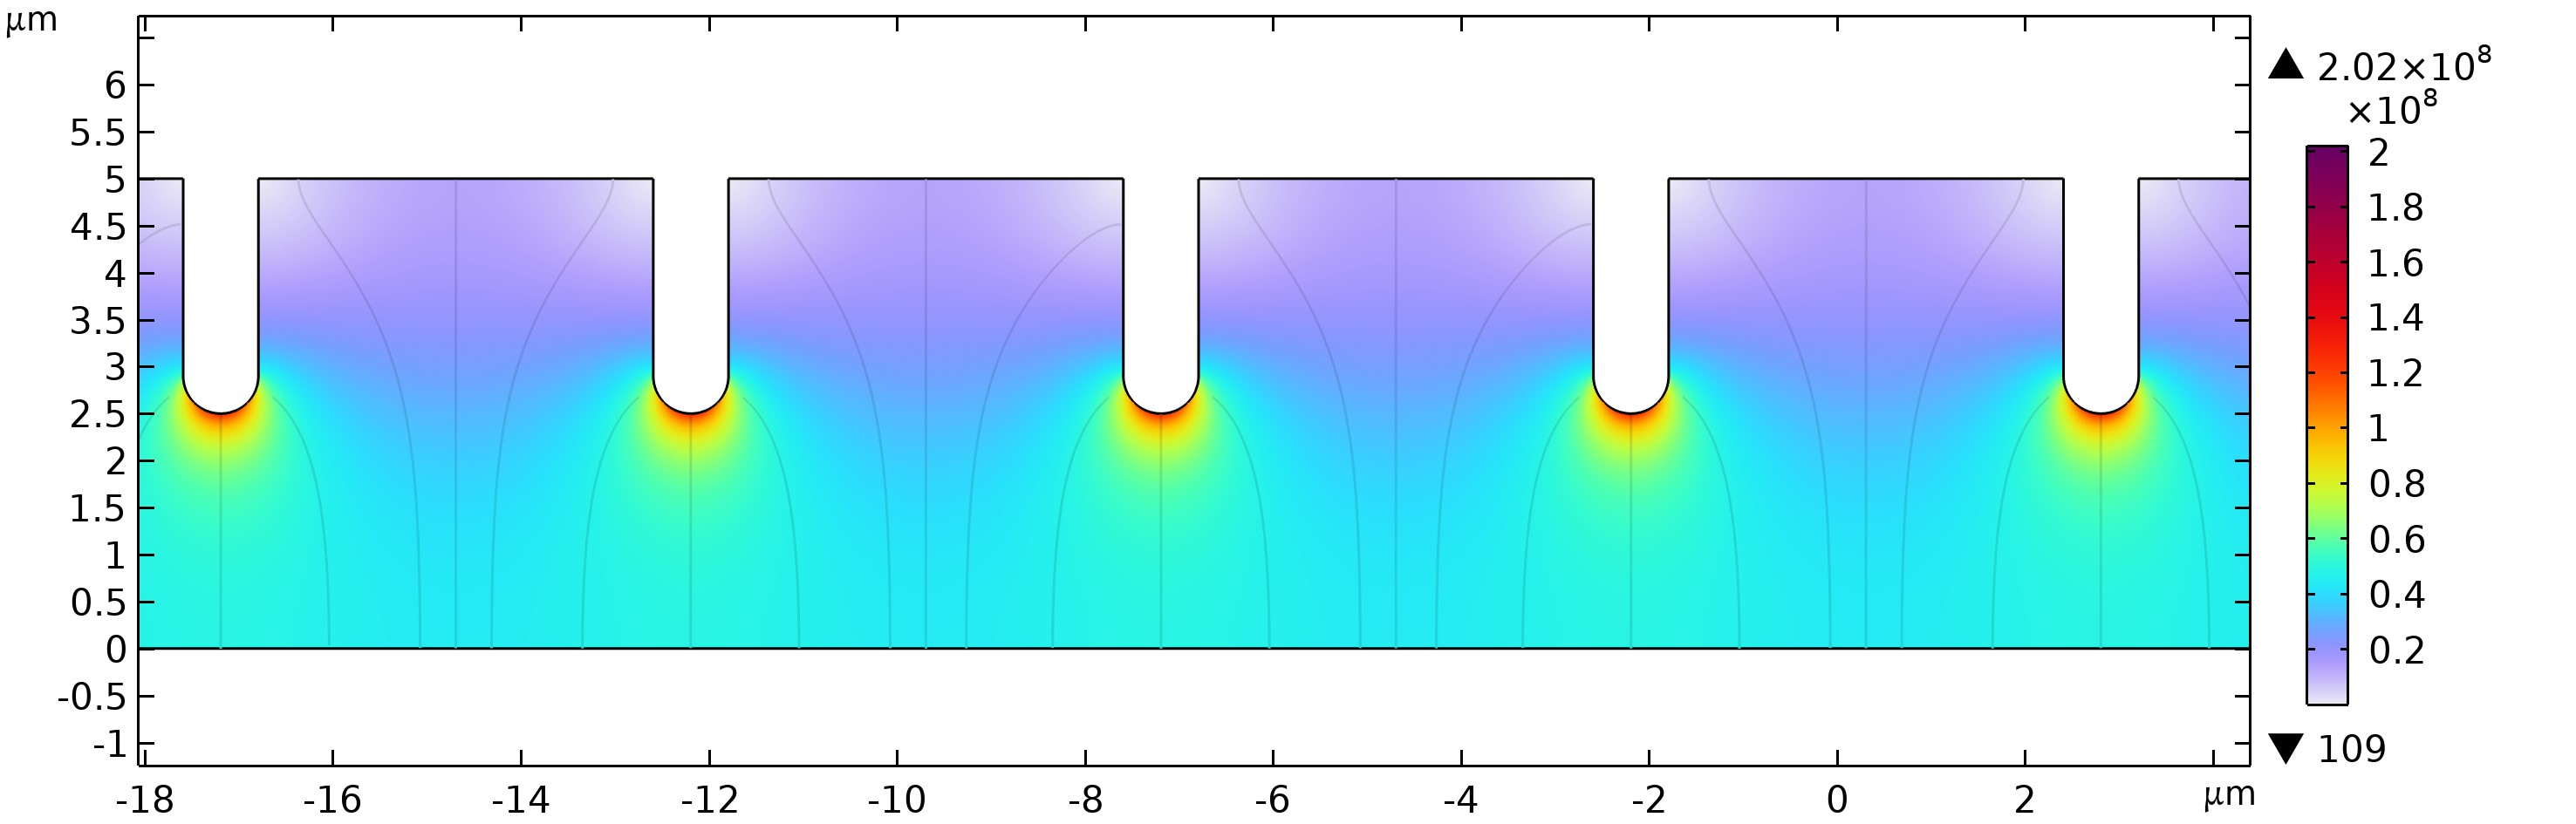
\includegraphics[width=\linewidth]{Chapter7/Figs/Raster/array_closer_es.jpg}
    \caption{The electric field norm of an idealised geometry for emitter array CH.}
    \label{fig:c_array_closer}
\end{figure}

Figure \ref{fig:c_array_closer} shows a closer view of the electrostatic model shown in figure \ref{fig:c_array_es_full}. At this scale, the emitters can be seen to have consistent tip electric field norms, with electric field lines only showing very minor deviations from perfect symmetry between adjacent emitters.


\subsection{Single Emitter Electrostatics}
As the emitter array displays a consistent electric field norm across all emitters in the ideal geometry case, computation of a single emitter utilising an ideal Schottky barrier with the addition of a simple Murphy-Good field effect emission contribution was implemented. Additionally, an ionised dopant concentration of $4.2\times10^{14}$~\si{\per\centi\metre\cubed} was applied to the diamond channel region.

\begin{figure}[H]
    \centering
    % Top left figure (1)
    \begin{subfigure}[b]{0.45\linewidth}
        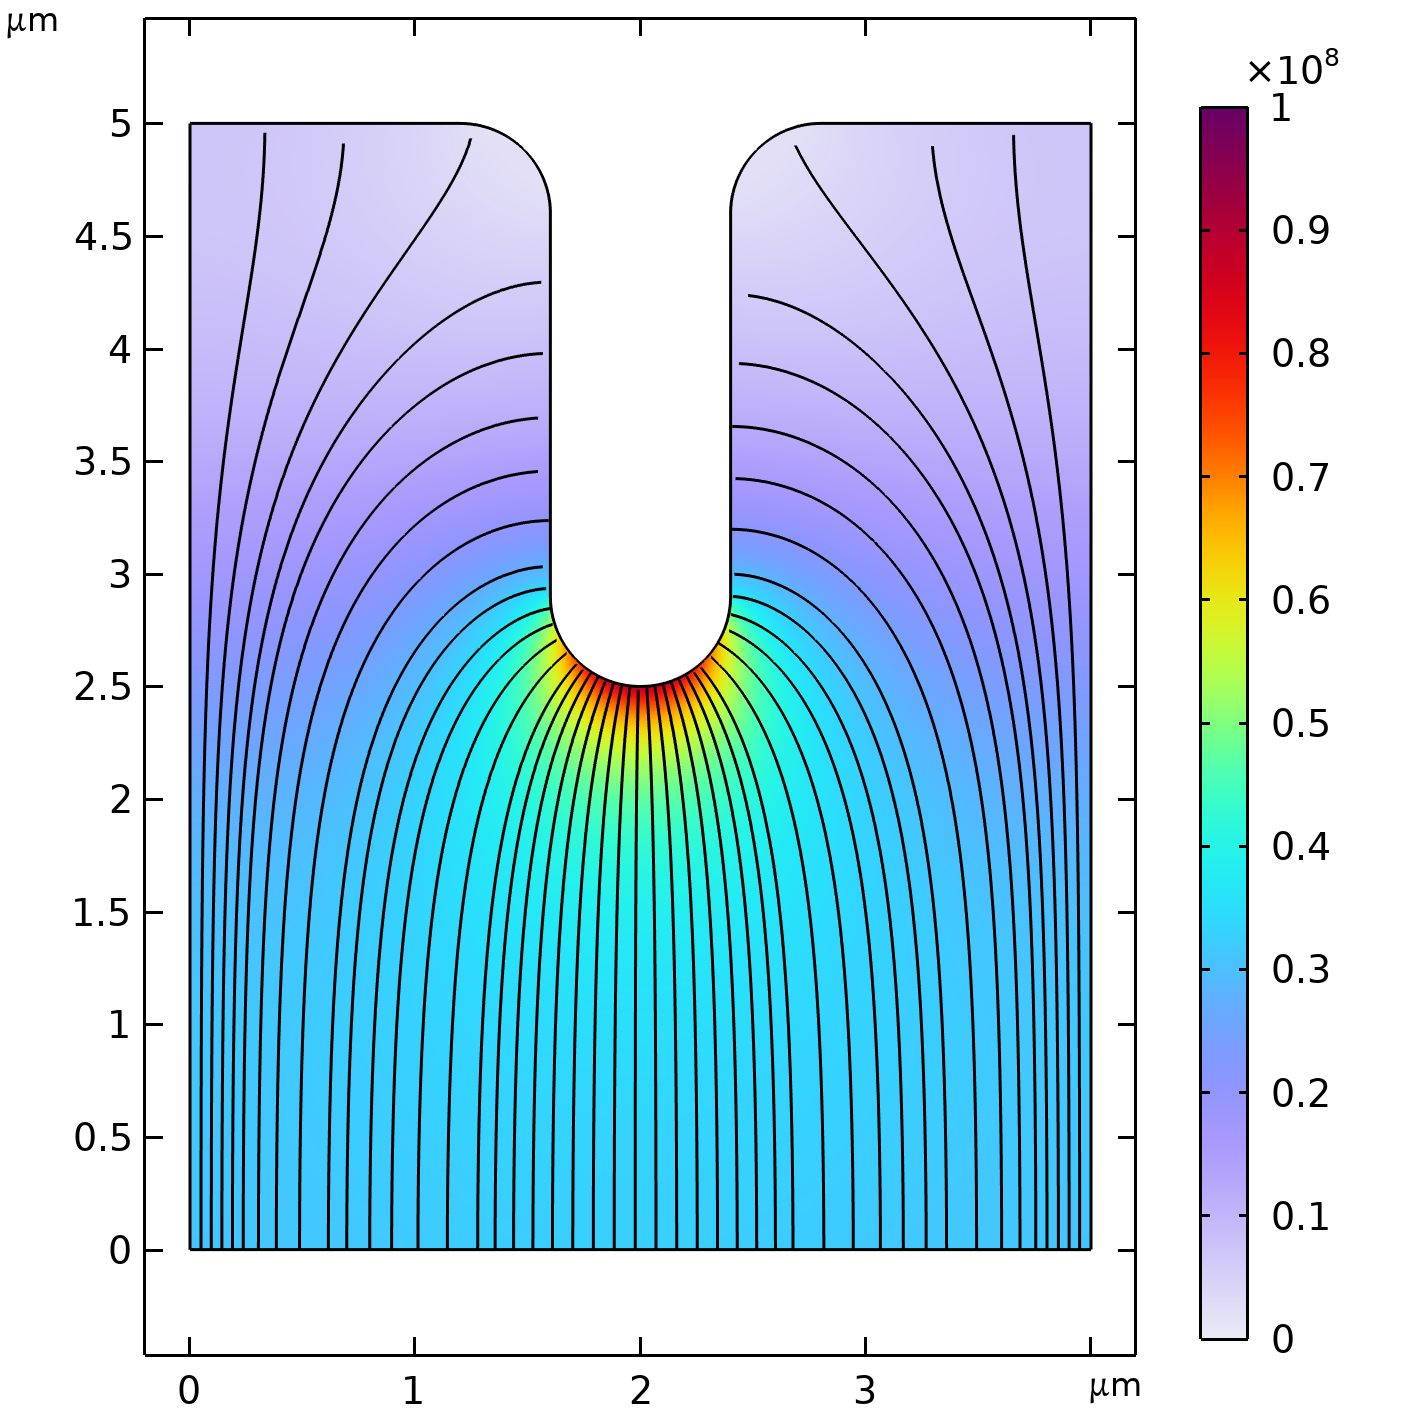
\includegraphics[width=\linewidth]{Chapter7/Figs/Raster/Comsol/+100_normE_smol.png}
        \caption{Linear $+100$~\si{\volt}.}
        \label{fig:c_+100_lin_norme}
    \end{subfigure}
    \hfill % this will insert a non-breaking space between the figures
    % Top right figure (2)
    \begin{subfigure}[b]{0.45\linewidth}
        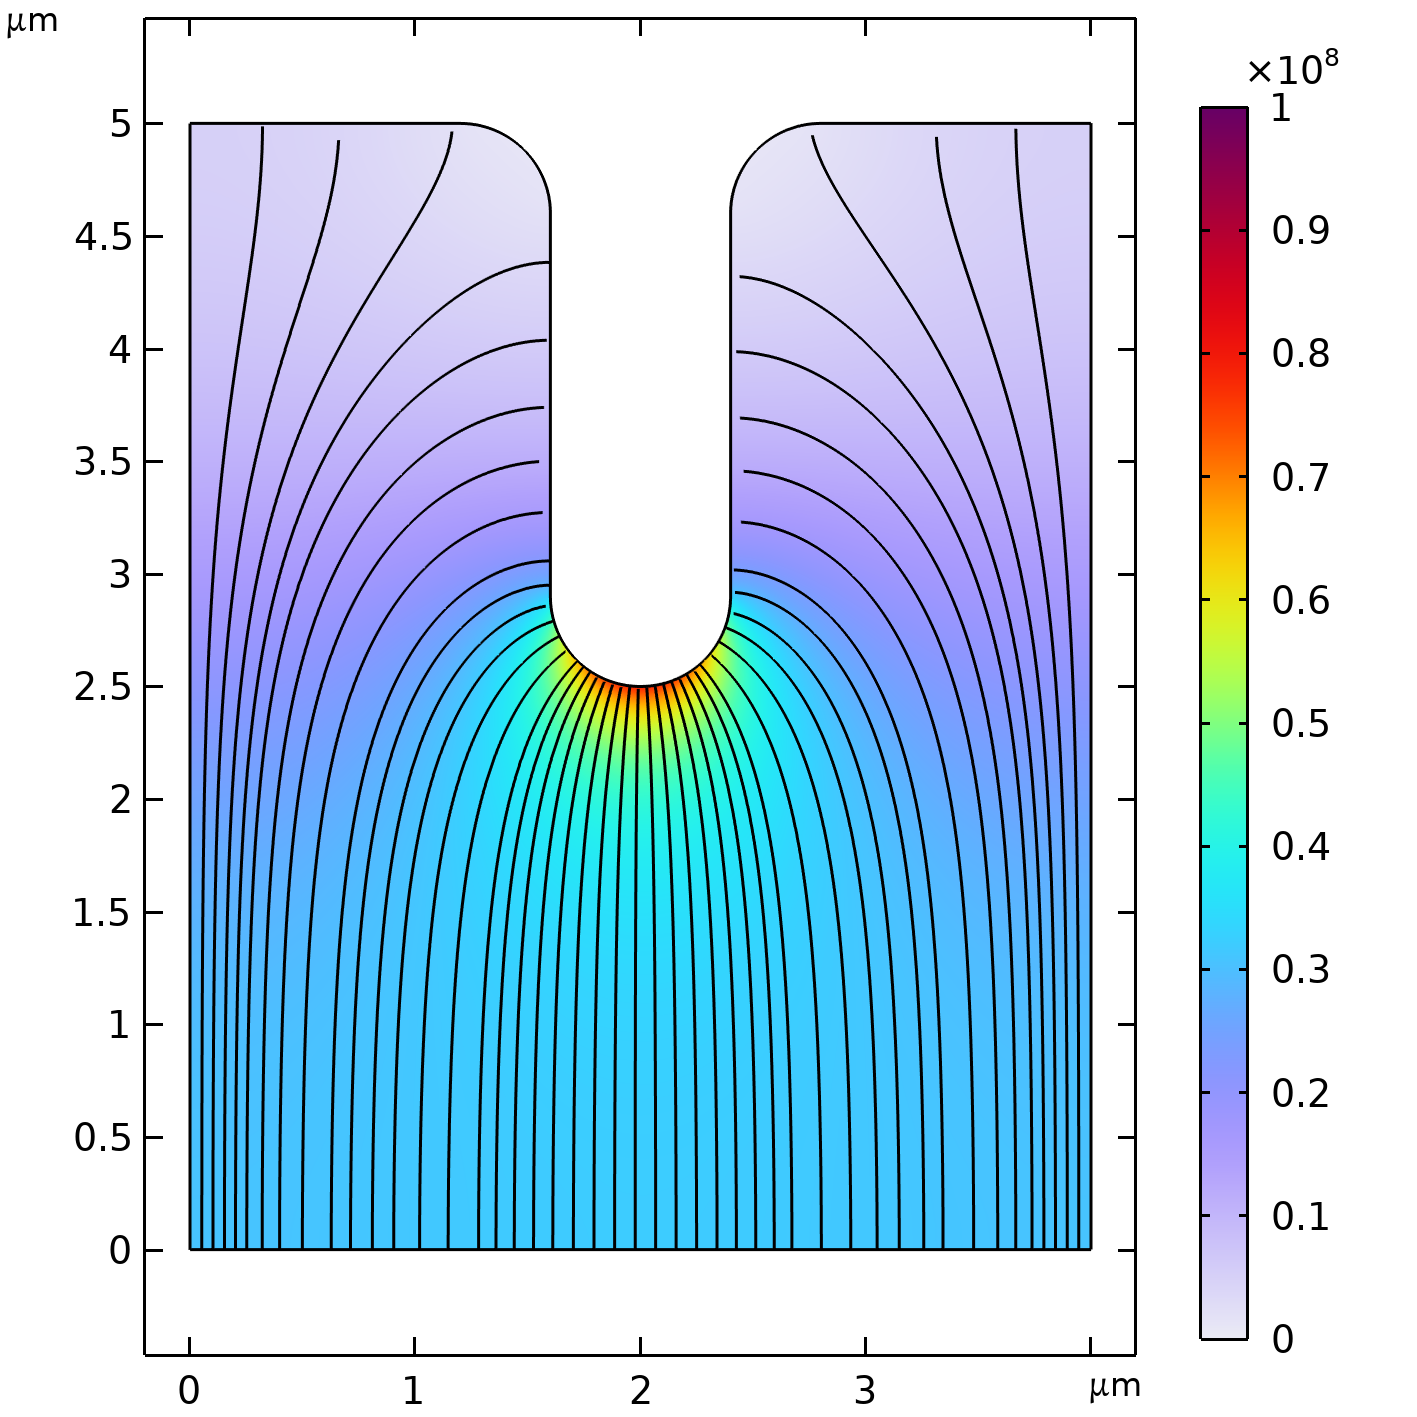
\includegraphics[width=\linewidth]{Chapter7/Figs/Raster/Comsol/-100_normE_smol.png}
        \caption{Linear $-100$~\si{\volt}.}
        \label{fig:c_-100_lin_norme}
    \end{subfigure}
    
    % Bottom left figure (3)
    \begin{subfigure}[b]{0.45\linewidth}
        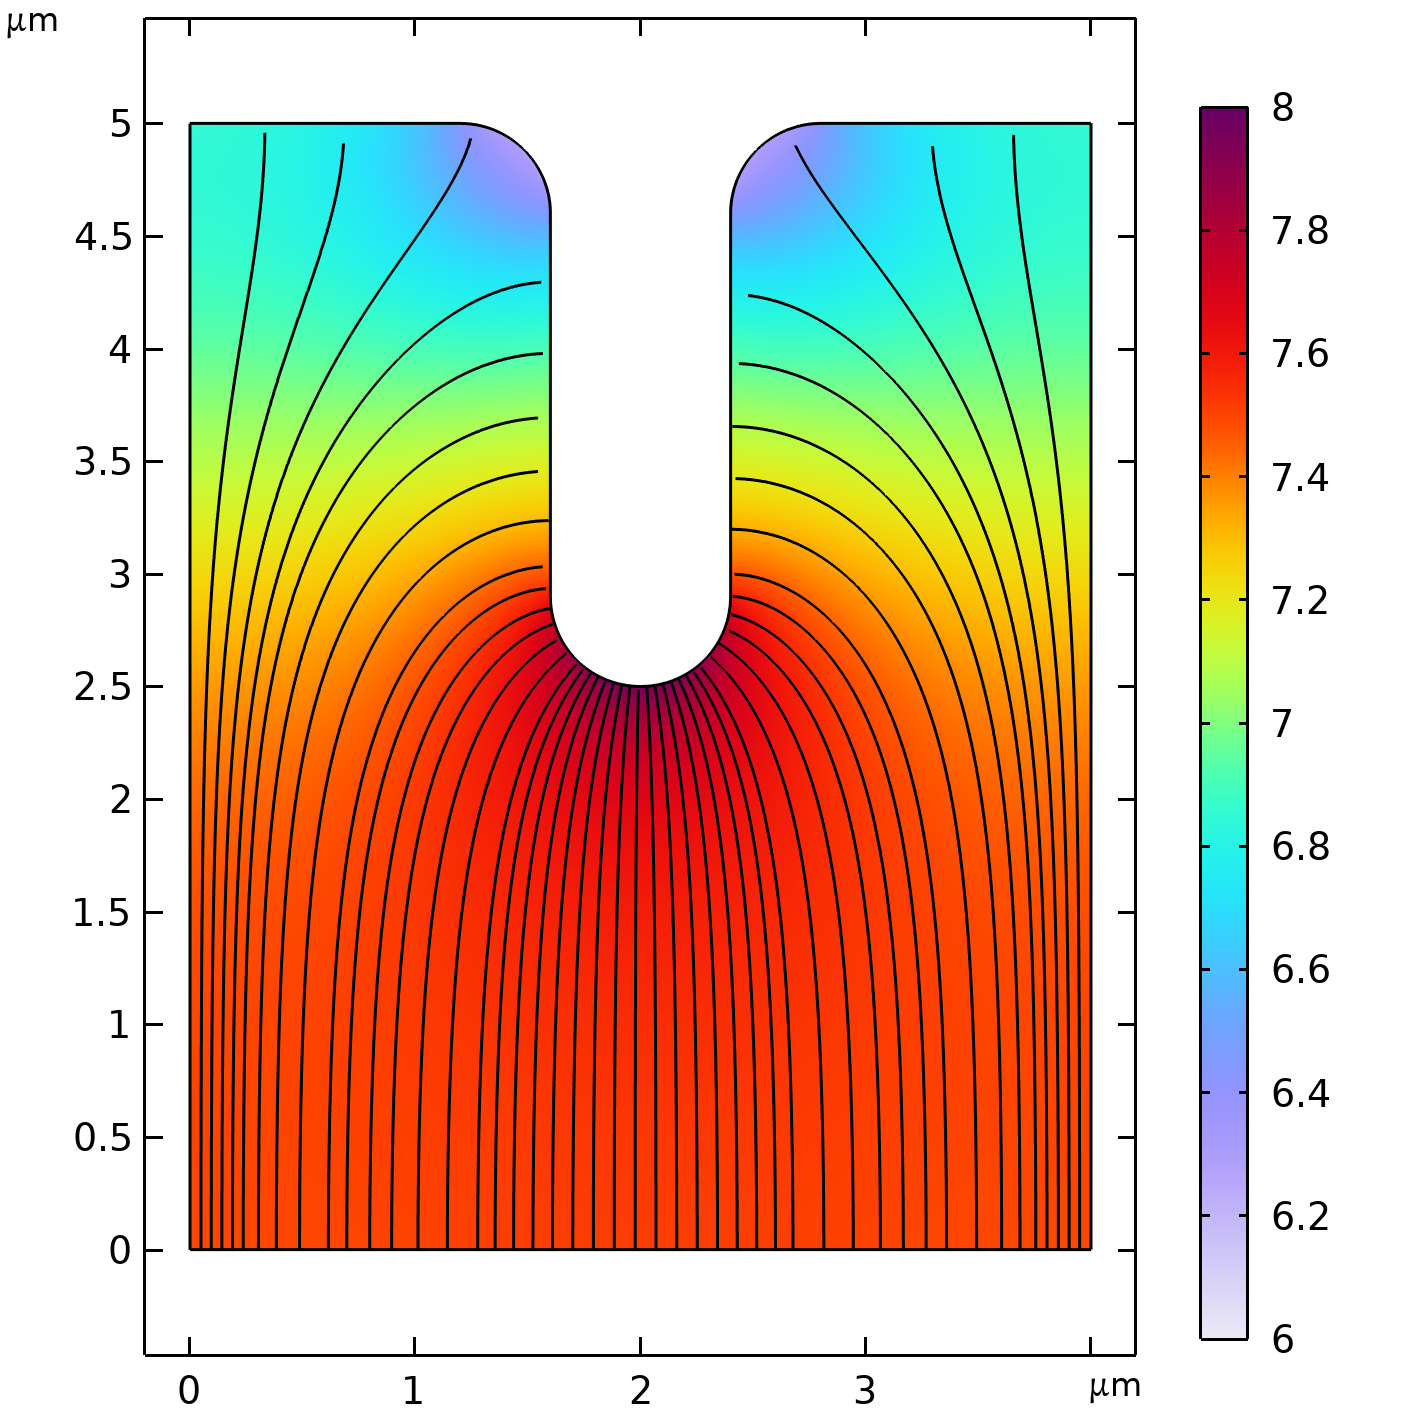
\includegraphics[width=\linewidth]{Chapter7/Figs/Raster/Comsol/+100_lognormE_smol.png}
        \caption{Log $+100$~\si{\volt}.}
        \label{fig:c_+100_log_norme}
    \end{subfigure}
    \hfill % this will insert a non-breaking space between the figures
    % Bottom right figure (4)
    \begin{subfigure}[b]{0.45\linewidth}
        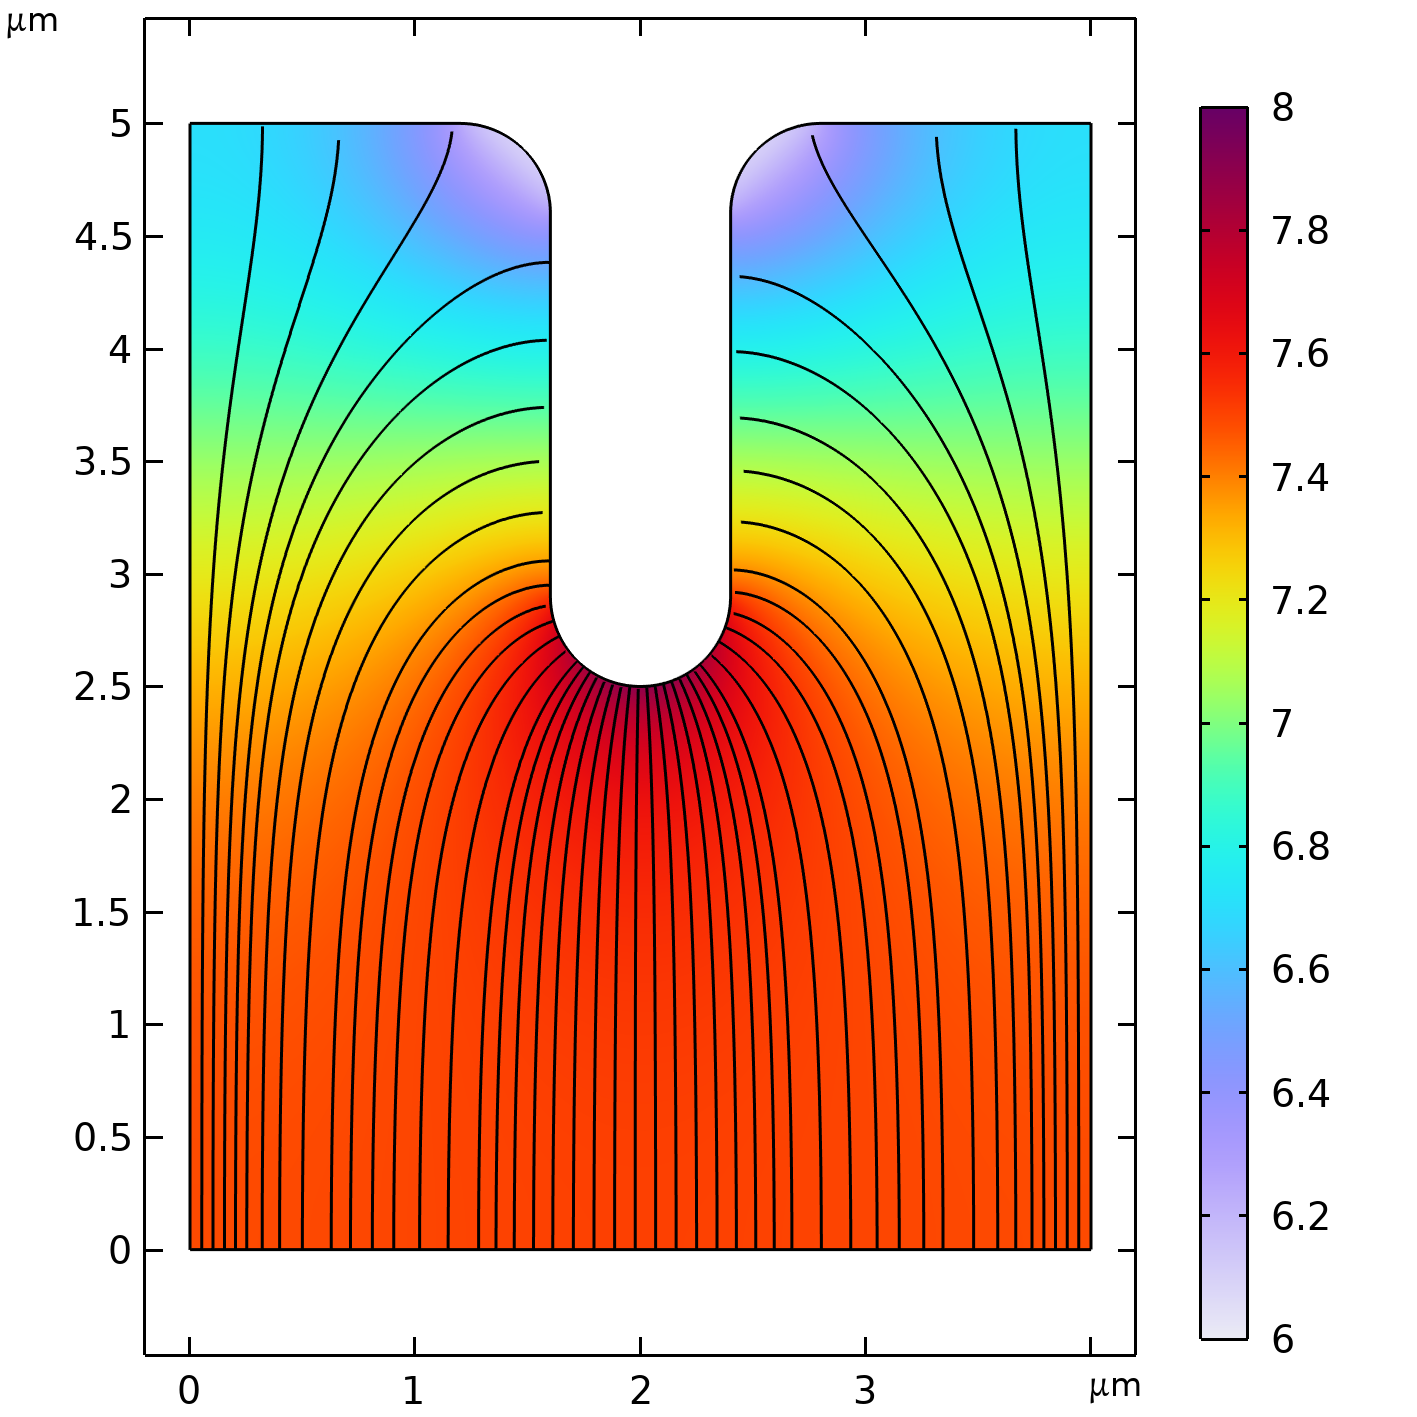
\includegraphics[width=\linewidth]{Chapter7/Figs/Raster/Comsol/-100_lognormE_smol.png}
        \caption{Log $-100$~\si{\volt}.}
        \label{fig:c_-100_log_norme}
    \end{subfigure}
    
    \caption{Electric field norm on the idealised emitter cathode.}
    \label{fig:electric_field_norm}
\end{figure}

Figure \ref{fig:electric_field_norm} presents both the electric field norm at maximum (left column) and minimum (right column) applied anode biases in a linear (top row) and log (bottom row) scale form for ease of visual comparison. Streamlines representing the magnitude of the electric field are included to provide further visualisation of the localisation of electric field on the emitter tips. Both extremes of potential bias in this model show a reasonably similar distribution and magnitude of electric field norm, with only a minor deviation seen as an increase of the peak cathode electric field norm in the positive bias case, as opposed to the negatively biased anode case. 

\subsection{Single Emitter Field Emission}
\begin{figure}[H]
    \centering
    % Top left figure (1)
    \begin{subfigure}[b]{0.45\linewidth}
        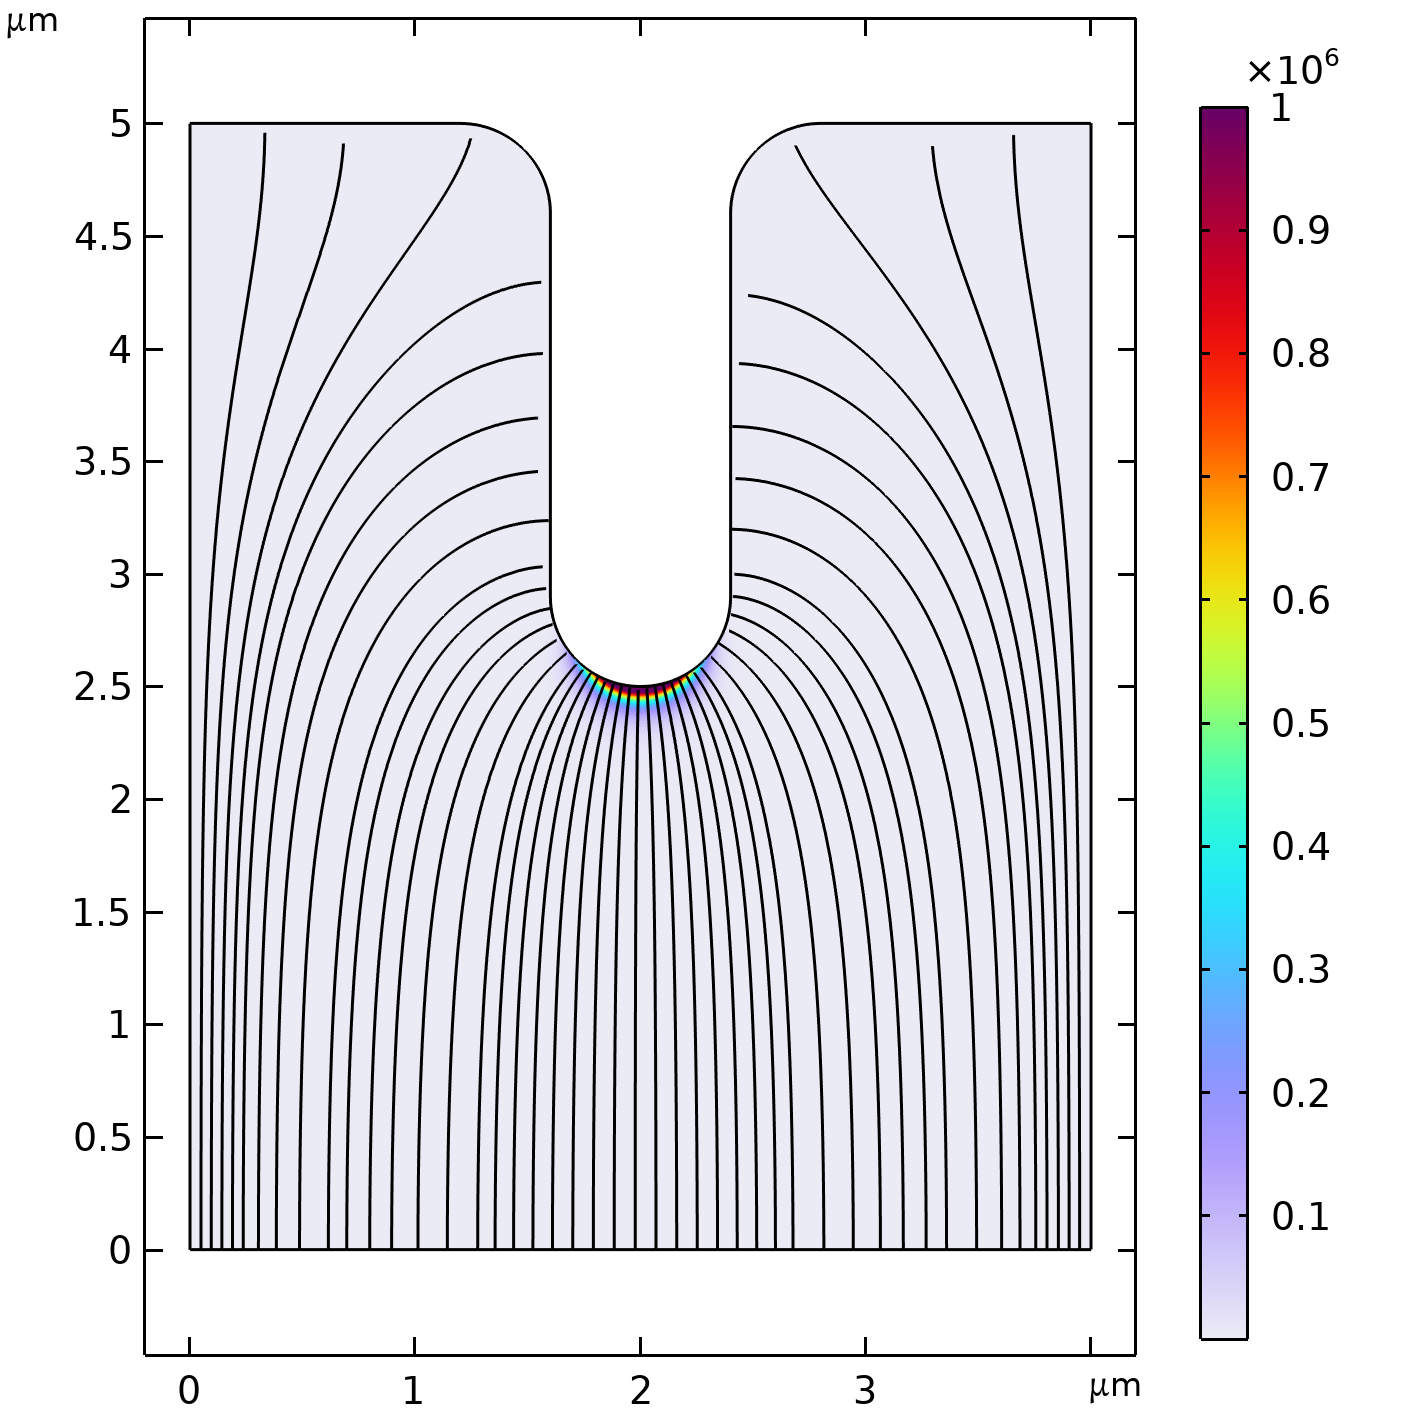
\includegraphics[width=\linewidth]{Chapter7/Figs/Raster/Comsol/+100_J_GM_smol.png}
        \caption{Linear $+100$~\si{\volt}.}
        \label{fig:c_+100_j_gm}
    \end{subfigure}
    \hfill % this will insert a non-breaking space between the figures
    % Top right figure (2)
    \begin{subfigure}[b]{0.45\linewidth}
        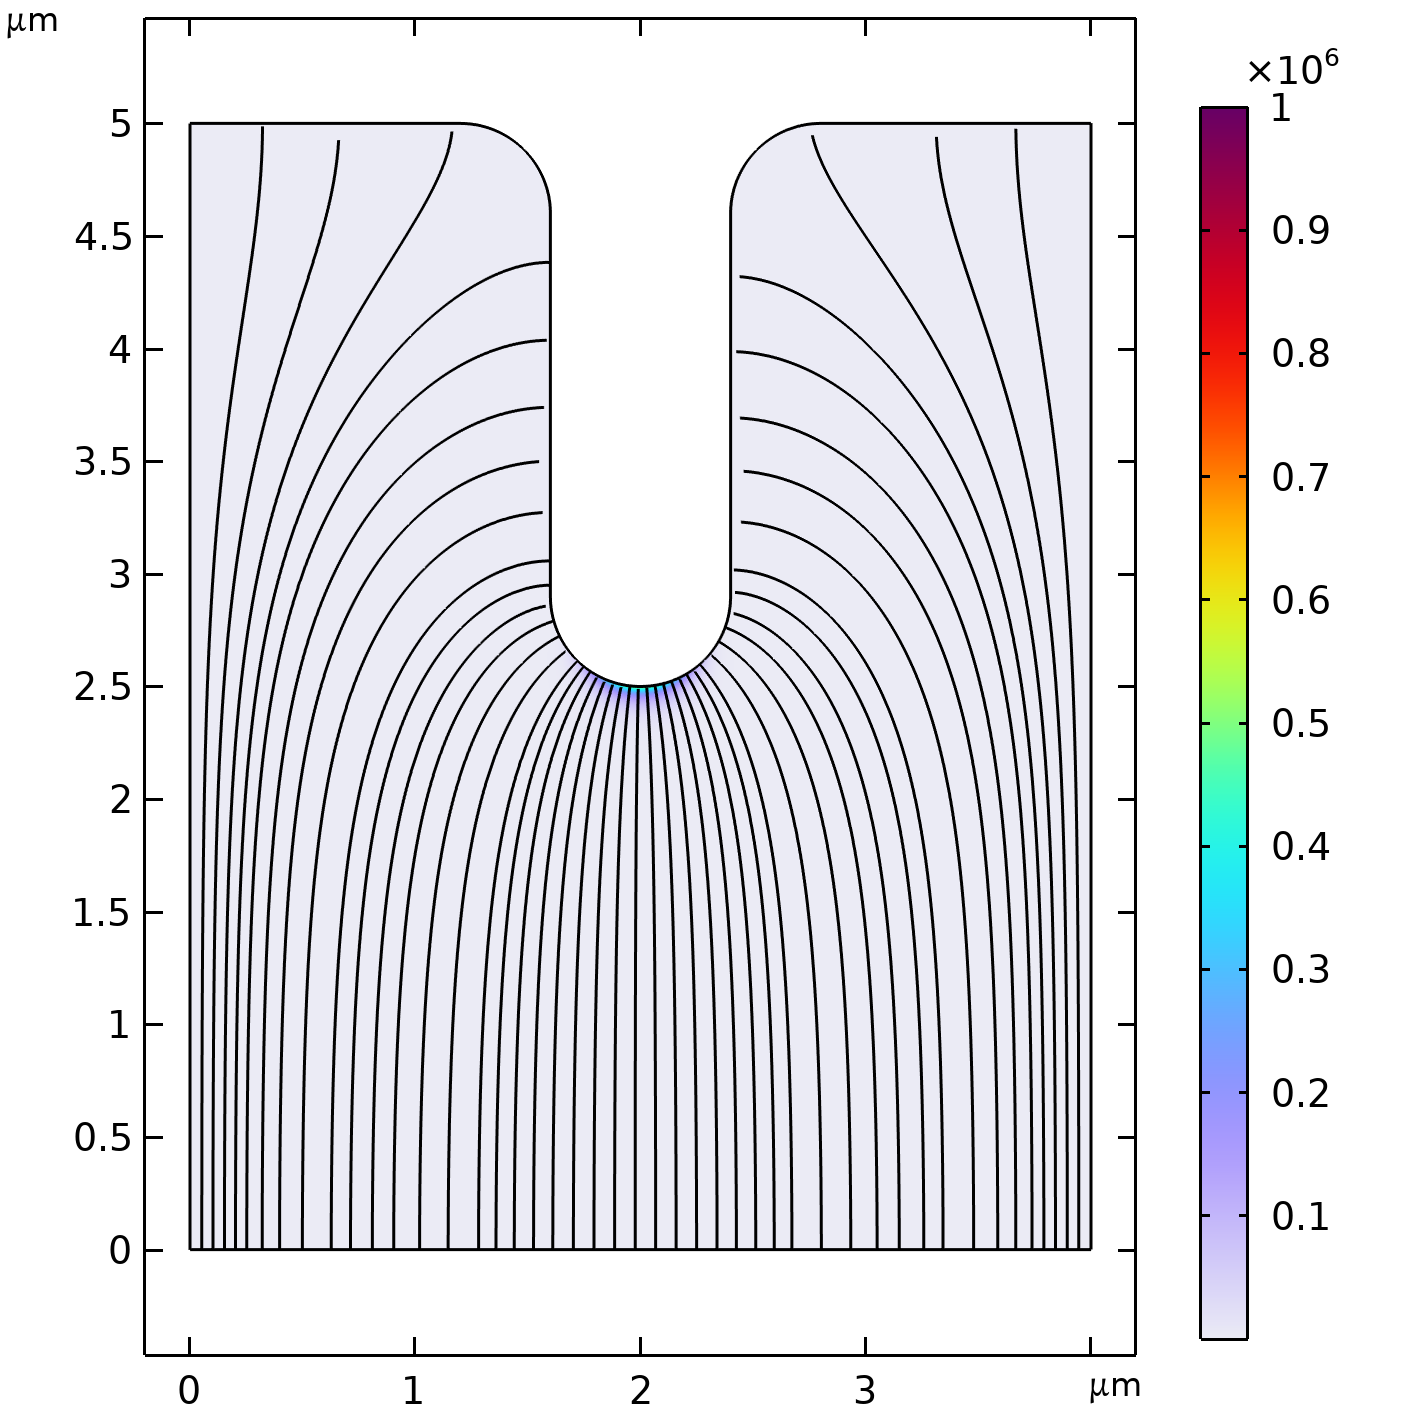
\includegraphics[width=\linewidth]{Chapter7/Figs/Raster/Comsol/-100_J_GM_smol.png}
        \caption{Linear $-100$~\si{\volt}.}
        \label{fig:c_-100_lin_j_gm}
    \end{subfigure}
    
    % Bottom left figure (3)
    \begin{subfigure}[b]{0.45\linewidth}
        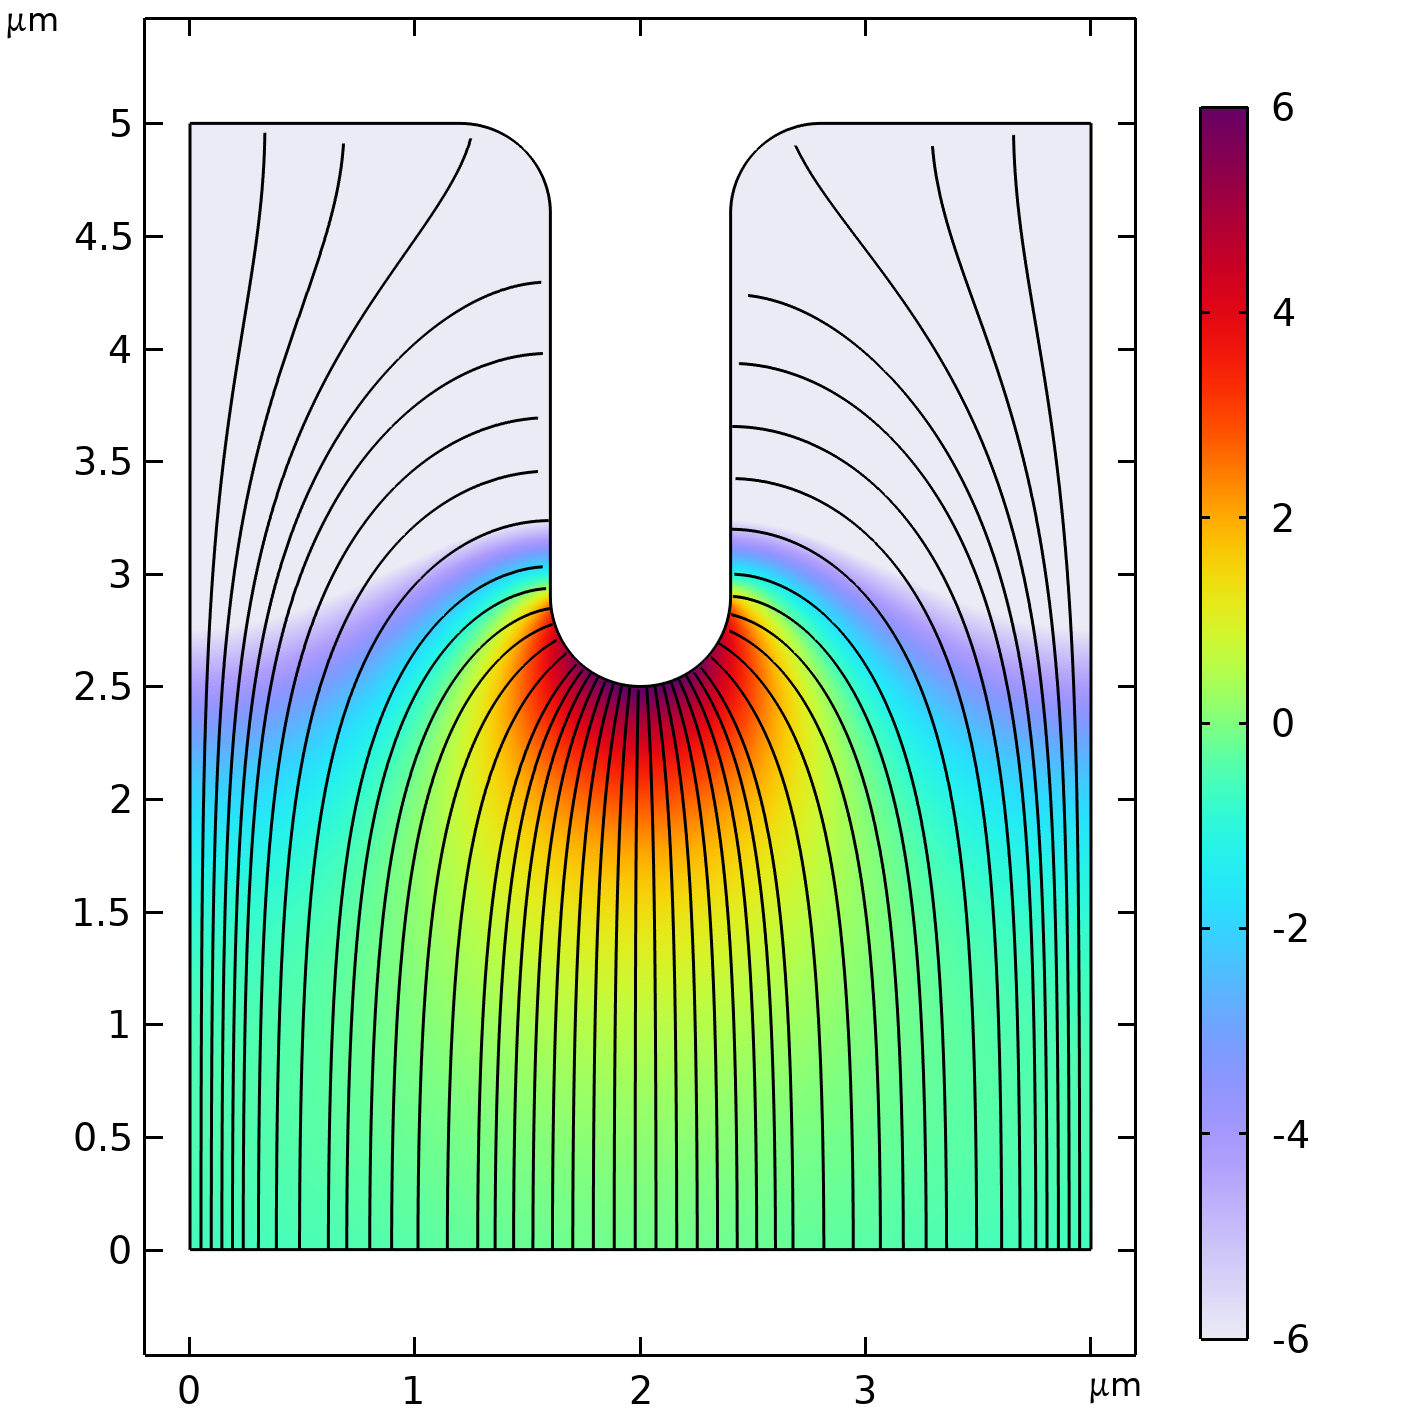
\includegraphics[width=\linewidth]{Chapter7/Figs/Raster/Comsol/+100_logJ_GM_smol.png}
        \caption{Log $+100$~\si{\volt}.}
        \label{fig:c_+100_log_j_gm}
    \end{subfigure}
    \hfill % this will insert a non-breaking space between the figures
    % Bottom right figure (4)
    \begin{subfigure}[b]{0.45\linewidth}
        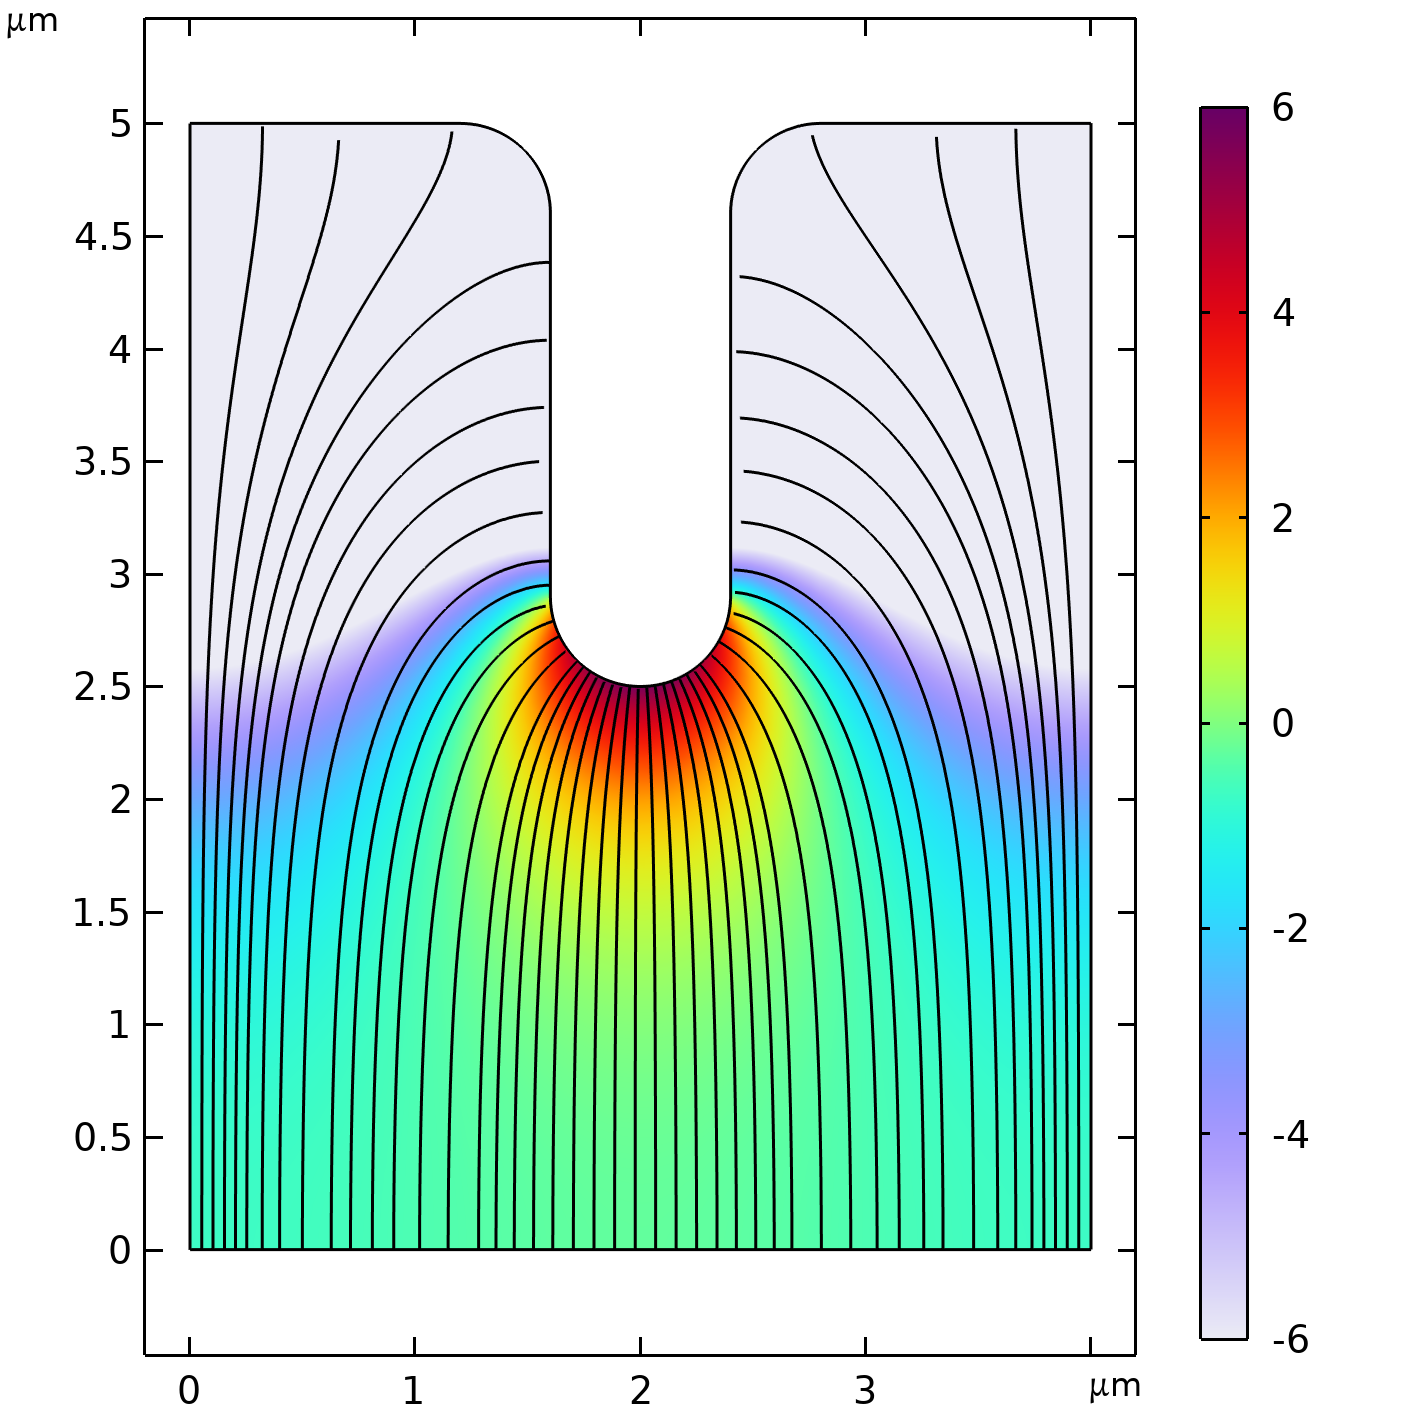
\includegraphics[width=\linewidth]{Chapter7/Figs/Raster/Comsol/-100_logJ_GM_smol.png}
        \caption{Log $-100$~\si{\volt}.}
        \label{fig:c_-100_log_j_gm}
    \end{subfigure}
    
    \caption{Simple Murphy-Good current density for idealised emitter cathode.}
    \label{fig:field_emission}
\end{figure}

Figure \ref{fig:field_emission} shows the results of applying the Murphy-Good field effect emission current density to the single emitter geometry. As for figure \ref{fig:electric_field_norm}, the top row shows the linear scale plot, while the bottom row shows the log scale plot of current density. Overall, it can be seen that the positive and negative applied anode voltages only have a slight impact upon the observed field effect emission, with a greater emission in the positive region. The emission is concentrated quite strongly upon the very apex of the emitter in both cases too, showing that the exact geometry of these cathode structures may have a large impact upon the profile of field effect emission. While this is an idealised geometry, it is quite evident that an irregular geometry will have a complex field emission profile, and it is entirely possible that sharper regions at a greater cathode-anode spacing may result in an appreciable field effect emission contribution. 

\subsection{Comparison of Schottky and Field Emission Current}
\begin{wrapfigure}{l}{0.5\linewidth}
    \centering
    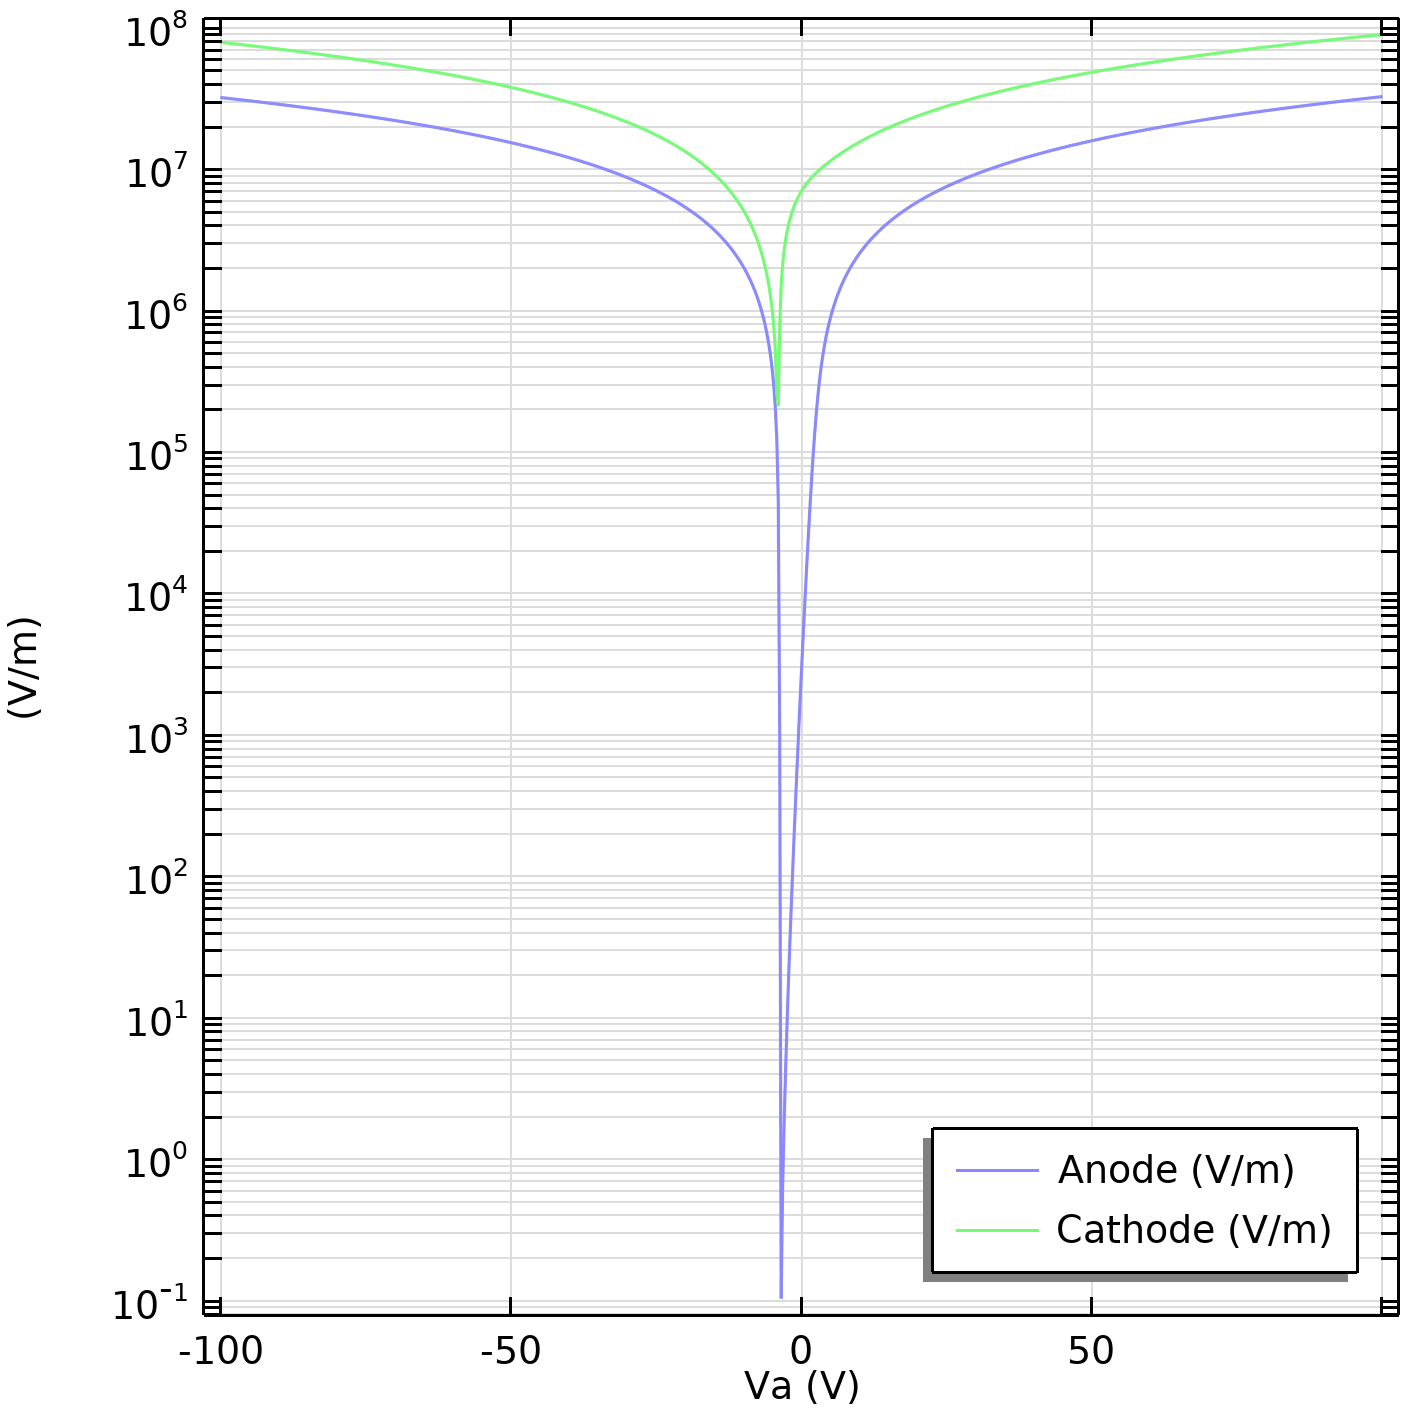
\includegraphics[width=\linewidth]{Chapter7/Figs/Raster/Comsol/cathode_anode_comparison.png}
    \caption{The peak electric field norm on both the anode and cathode for $\pm150$~\si{\volt}.}
    \label{fig:c_cathode_anode_comparison}
\end{wrapfigure}

With the ideal single emitter model as described thus far, the resulting thermionic and field effect current densities can be analysed to consider whether this ideal model represents the experimental data in any capacity. In figure \ref{fig:c_cathode_anode_comparison}, an additional electrostatic comparison of the cathode and anode is plotted for a bias range of $\pm100$~\si{\volt}. The cathode has a distinctly increased electric field norm at all applied potential biases, albeit around an order of magnitude. This may indicate that at high potential biases, the possibility of field effect emission occurring on the anode itself is possible, especially with geometries that are far from ideal. Another noteworthy feature of this plot is the off-centre minima for both electrodes, which is due to charge accumulation on the cathode and anode. This is not reflected in simpler electrostatic modelling used for the array structure, and presents an ionised dopant dependency upon the electric field norm. While this model does not implement a model of band bending, it is an interesting result that surface accumulation is observed to affect the field effect emission without specifically including approximations to account for this factor.

\begin{figure}[H]
    \centering
    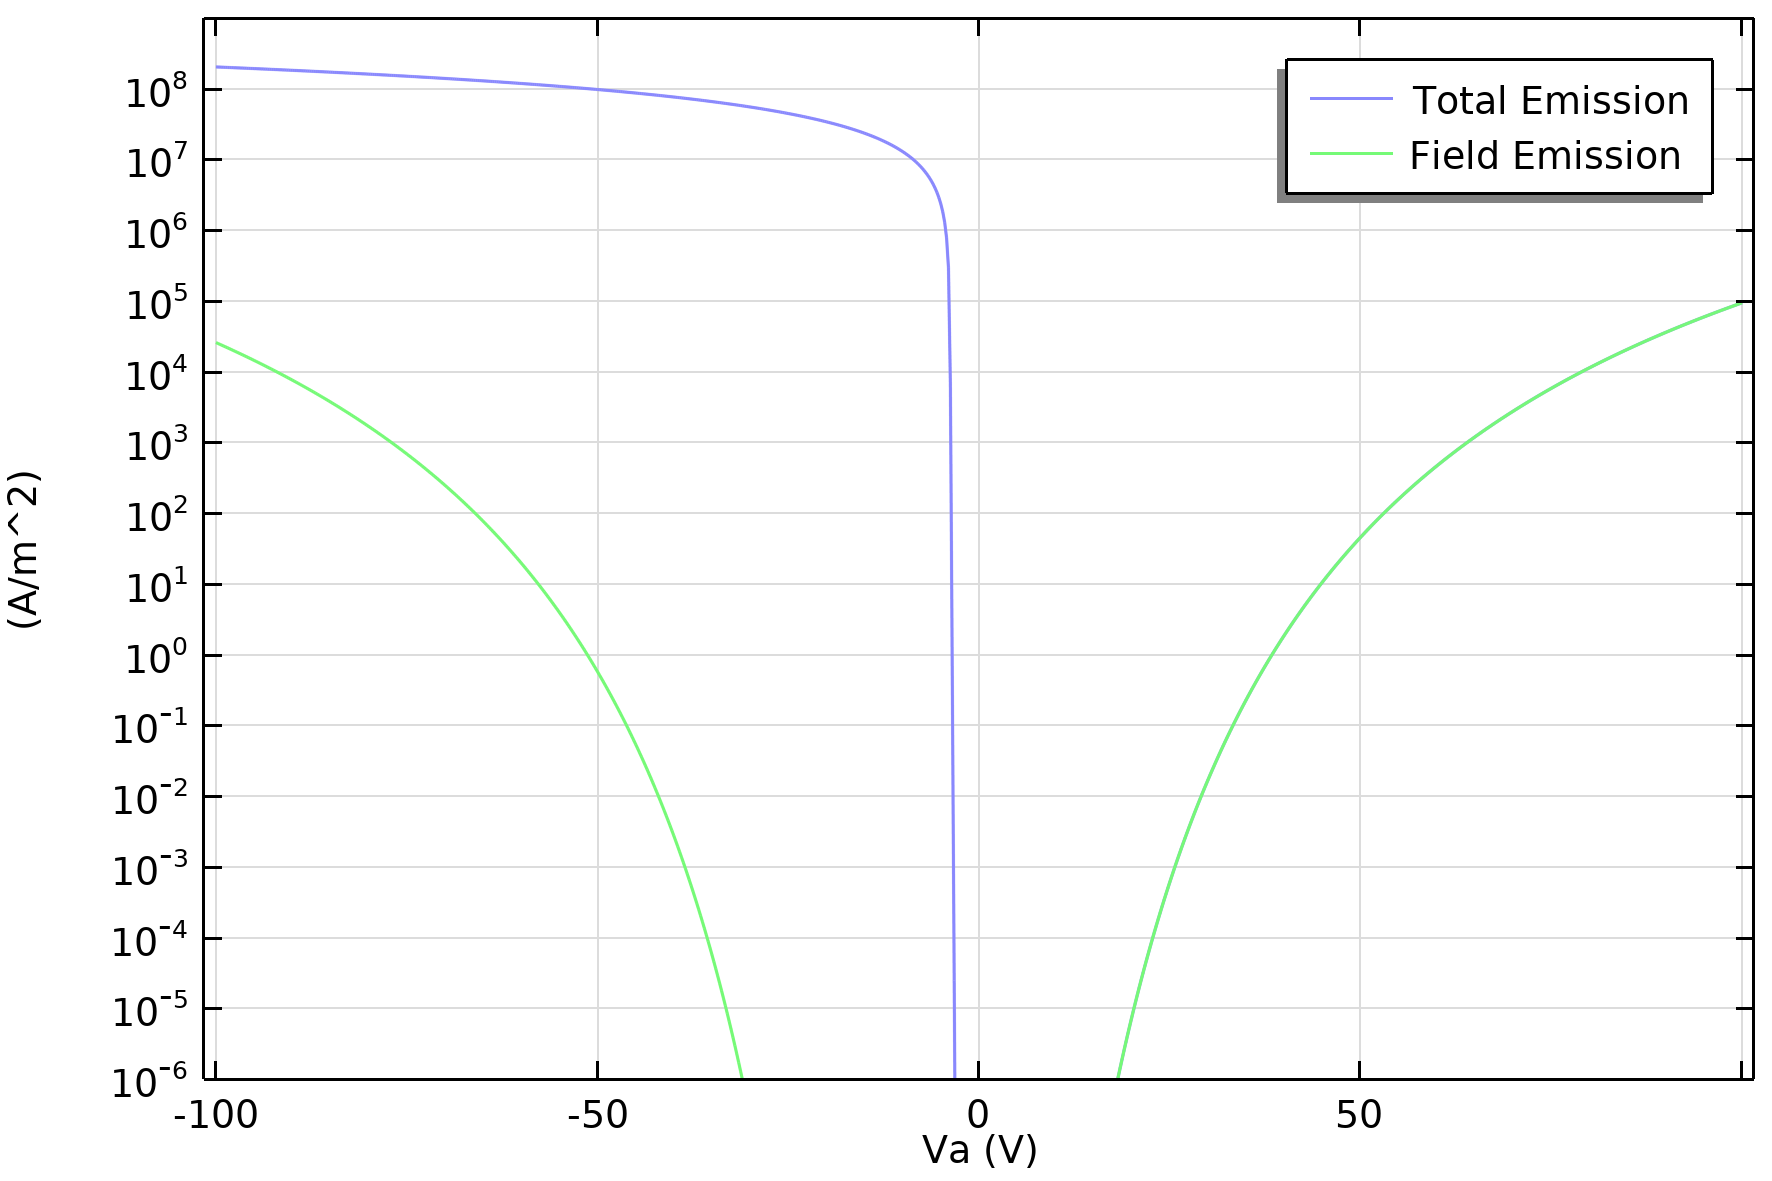
\includegraphics[width=0.8\linewidth]{Chapter7/Figs/Raster/Comsol/density_thermionic_field_comparison.png}
    \caption{The total and field emission current densities from the cathode for anode biases of -100 to +100~\si{\volt}.}
    \label{fig:c_density_thermionic_field_comparison}
\end{figure}

In figure \ref{fig:c_density_thermionic_field_comparison}, the total field effect emission current densities are compared over the cathode boundary. As modelled, the ideal Schottky barrier appears to present a much stronger source of current density across the negative bias region, due to the forward bias producing a strong thermionic emission current, but the field effect emission contribution is growing in significance at the highest magnitude of negatively applied potential bias. Note that in the positive region of the plot, the total current density represents the positively biased field effect emission current density, and the lines overlap exactly. This is due to the Schottky cathode being in reverse bias in this bias region, hence the effective saturation current is entirely made up of the field effect contribution.

\begin{figure}[H]
    \centering
    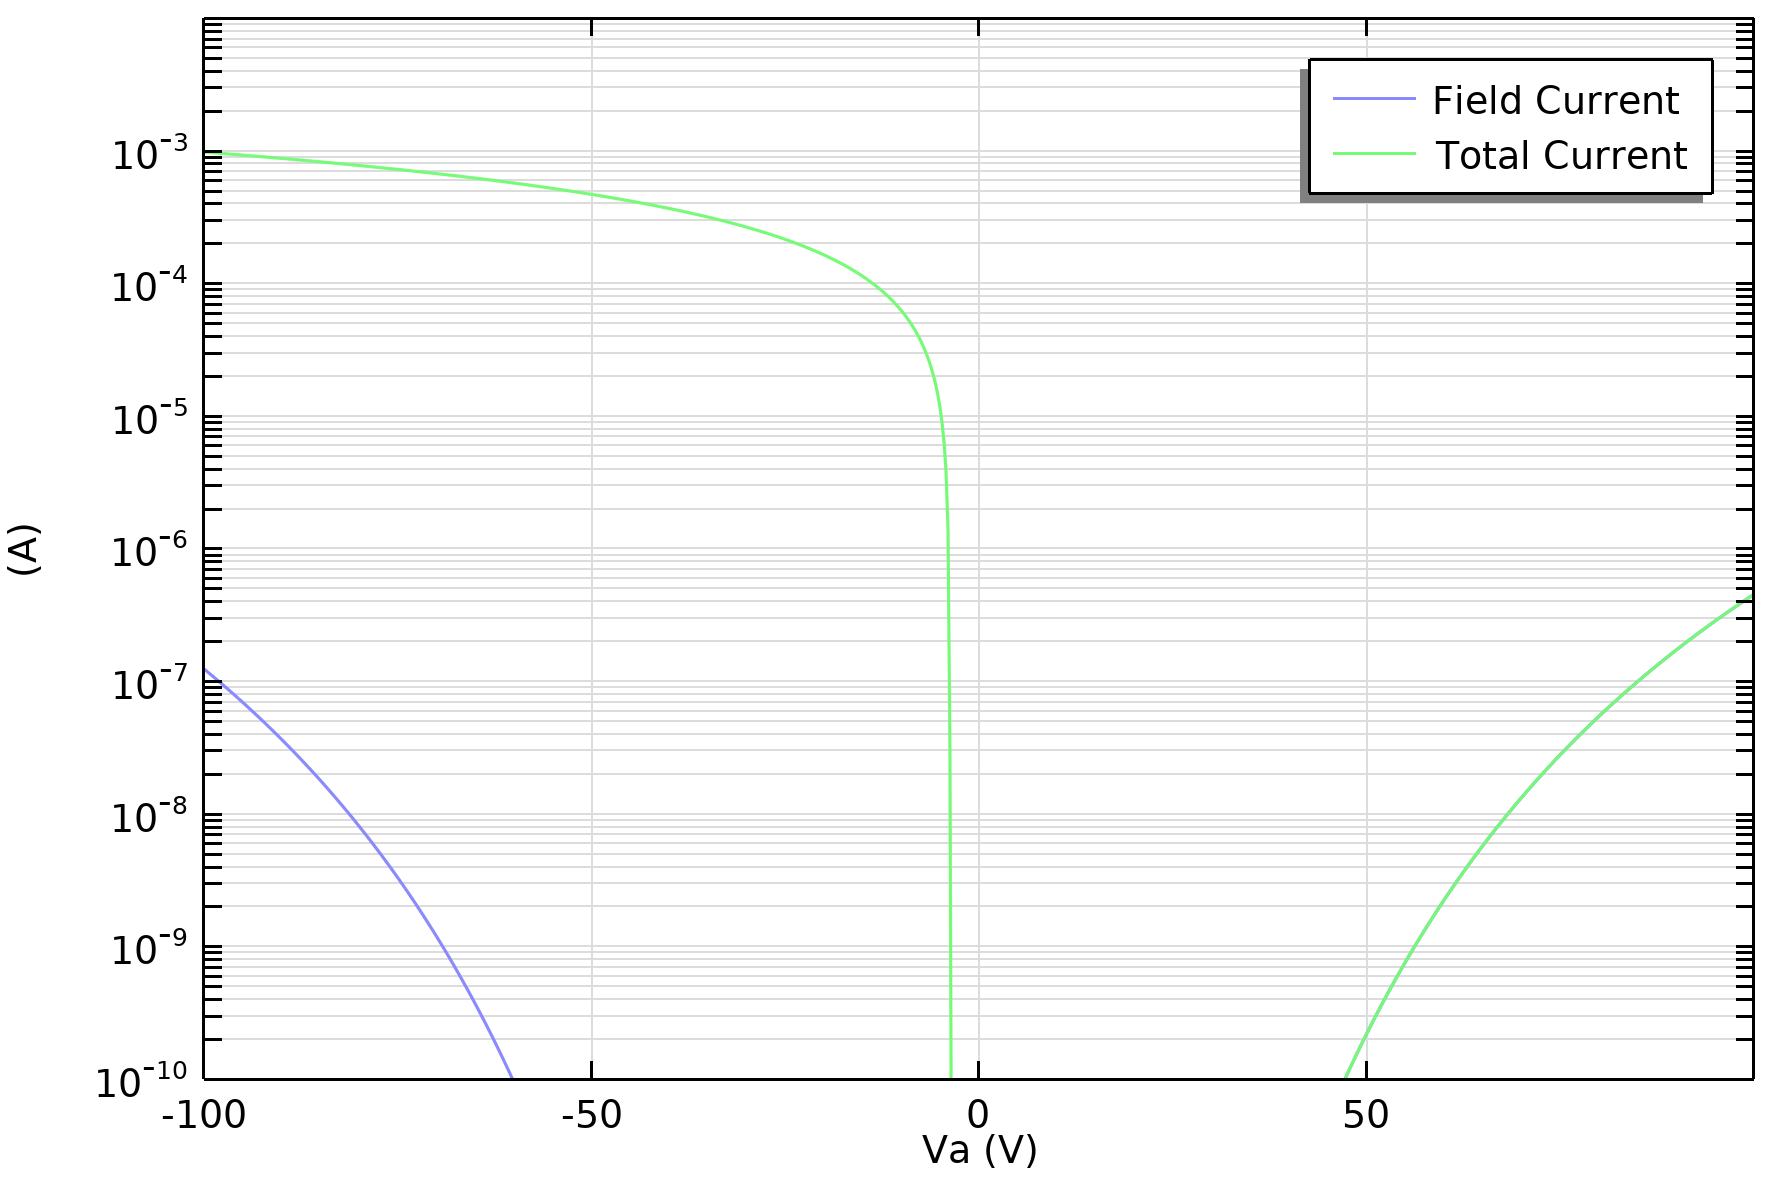
\includegraphics[width=0.8\linewidth]{Chapter7/Figs/Raster/Comsol/current_thermionic_field_comparison.png}
    \caption{The total and field emission integrated current from the cathode for anode biases of -100 to +100~\si{\volt}.}
    \label{fig:c_current_thermionic_field_comparison}
\end{figure}

Figure \ref{fig:c_current_thermionic_field_comparison} presents the integrated effective current over the cathode, with the total current plotted alongside the current contribution directly from field effect emission. As this is directly dependent upon the emission current density, it is no surprise that the integrated current follows a similar trend as for figure \ref{fig:c_density_thermionic_field_comparison}, with a dominant forwardly biased Schottky barrier in the negative bias region and a relatively minor contribution from the field emission element in both bias directions.

\printbibliography[heading=subbibliography]

\end{refsection}